\documentclass[twoside]{book}

% Packages required by doxygen
\usepackage{fixltx2e}
\usepackage{calc}
\usepackage{doxygen}
\usepackage[export]{adjustbox} % also loads graphicx
\usepackage{graphicx}
\usepackage[utf8]{inputenc}
\usepackage{makeidx}
\usepackage{multicol}
\usepackage{multirow}
\PassOptionsToPackage{warn}{textcomp}
\usepackage{textcomp}
\usepackage[nointegrals]{wasysym}
\usepackage[table]{xcolor}

% Font selection
\usepackage[T1]{fontenc}
\usepackage[scaled=.90]{helvet}
\usepackage{courier}
\usepackage{amssymb}
\usepackage{sectsty}
\renewcommand{\familydefault}{\sfdefault}
\allsectionsfont{%
  \fontseries{bc}\selectfont%
  \color{darkgray}%
}
\renewcommand{\DoxyLabelFont}{%
  \fontseries{bc}\selectfont%
  \color{darkgray}%
}
\newcommand{\+}{\discretionary{\mbox{\scriptsize$\hookleftarrow$}}{}{}}

% Page & text layout
\usepackage{geometry}
\geometry{%
  a4paper,%
  top=2.5cm,%
  bottom=2.5cm,%
  left=2.5cm,%
  right=2.5cm%
}
\tolerance=750
\hfuzz=15pt
\hbadness=750
\setlength{\emergencystretch}{15pt}
\setlength{\parindent}{0cm}
\setlength{\parskip}{0.2cm}
\makeatletter
\renewcommand{\paragraph}{%
  \@startsection{paragraph}{4}{0ex}{-1.0ex}{1.0ex}{%
    \normalfont\normalsize\bfseries\SS@parafont%
  }%
}
\renewcommand{\subparagraph}{%
  \@startsection{subparagraph}{5}{0ex}{-1.0ex}{1.0ex}{%
    \normalfont\normalsize\bfseries\SS@subparafont%
  }%
}
\makeatother

% Headers & footers
\usepackage{fancyhdr}
\pagestyle{fancyplain}
\fancyhead[LE]{\fancyplain{}{\bfseries\thepage}}
\fancyhead[CE]{\fancyplain{}{}}
\fancyhead[RE]{\fancyplain{}{\bfseries\leftmark}}
\fancyhead[LO]{\fancyplain{}{\bfseries\rightmark}}
\fancyhead[CO]{\fancyplain{}{}}
\fancyhead[RO]{\fancyplain{}{\bfseries\thepage}}
\fancyfoot[LE]{\fancyplain{}{}}
\fancyfoot[CE]{\fancyplain{}{}}
\fancyfoot[RE]{\fancyplain{}{\bfseries\scriptsize Generated on Mon Jun 8 2015 15\+:54\+:07 for Wave\+Blocks\+N\+D by Doxygen }}
\fancyfoot[LO]{\fancyplain{}{\bfseries\scriptsize Generated on Mon Jun 8 2015 15\+:54\+:07 for Wave\+Blocks\+N\+D by Doxygen }}
\fancyfoot[CO]{\fancyplain{}{}}
\fancyfoot[RO]{\fancyplain{}{}}
\renewcommand{\footrulewidth}{0.4pt}
\renewcommand{\chaptermark}[1]{%
  \markboth{#1}{}%
}
\renewcommand{\sectionmark}[1]{%
  \markright{\thesection\ #1}%
}

% Indices & bibliography
\usepackage{natbib}
\usepackage[titles]{tocloft}
\setcounter{tocdepth}{3}
\setcounter{secnumdepth}{5}
\makeindex

% Hyperlinks (required, but should be loaded last)
\usepackage{ifpdf}
\ifpdf
  \usepackage[pdftex,pagebackref=true]{hyperref}
\else
  \usepackage[ps2pdf,pagebackref=true]{hyperref}
\fi
\hypersetup{%
  colorlinks=true,%
  linkcolor=blue,%
  citecolor=blue,%
  unicode%
}

% Custom commands
\newcommand{\clearemptydoublepage}{%
  \newpage{\pagestyle{empty}\cleardoublepage}%
}


%===== C O N T E N T S =====

\begin{document}

% Titlepage & ToC
\hypersetup{pageanchor=false,
             bookmarks=true,
             bookmarksnumbered=true,
             pdfencoding=unicode
            }
\pagenumbering{roman}
\begin{titlepage}
\vspace*{7cm}
\begin{center}%
{\Large Wave\+Blocks\+N\+D }\\
\vspace*{1cm}
{\large Generated by Doxygen 1.8.9.1}\\
\vspace*{0.5cm}
{\small Mon Jun 8 2015 15:54:07}\\
\end{center}
\end{titlepage}
\clearemptydoublepage
\tableofcontents
\clearemptydoublepage
\pagenumbering{arabic}
\hypersetup{pageanchor=true}

%--- Begin generated contents ---
\chapter{Hierarchical Index}
\section{Class Hierarchy}
This inheritance list is sorted roughly, but not completely, alphabetically\+:\begin{DoxyCompactList}
\item \contentsline{section}{waveblocks\+:\+:Continuous\+Sqrt$<$ T $>$}{\pageref{classwaveblocks_1_1_continuous_sqrt}}{}
\item \contentsline{section}{waveblocks\+:\+:Continuous\+Sqrt$<$ real\+\_\+t $>$}{\pageref{classwaveblocks_1_1_continuous_sqrt}}{}
\item \contentsline{section}{waveblocks\+:\+:Tiny\+Multi\+Index$<$ U\+I\+N\+T, D $>$\+:\+:Entry}{\pageref{classwaveblocks_1_1_tiny_multi_index_1_1_entry}}{}
\item \contentsline{section}{std\+:\+:equal\+\_\+to$<$ waveblocks\+:\+:Tiny\+Multi\+Index$<$ U\+I\+N\+T, D $>$ $>$}{\pageref{structstd_1_1equal__to_3_01waveblocks_1_1_tiny_multi_index_3_01_u_i_n_t_00_01_d_01_4_01_4}}{}
\item \contentsline{section}{waveblocks\+:\+:Evaluator$<$ D, N $>$}{\pageref{classwaveblocks_1_1_evaluator}}{}
\item \contentsline{section}{waveblocks\+:\+:Extended\+Shape$<$ D, S $>$}{\pageref{classwaveblocks_1_1_extended_shape}}{}
\item \contentsline{section}{waveblocks\+:\+:Extended\+Shape$<$ D, Hyper\+Cubic\+Shape$<$ D $>$ $>$}{\pageref{classwaveblocks_1_1_extended_shape_3_01_d_00_01_hyper_cubic_shape_3_01_d_01_4_01_4}}{}
\item \contentsline{section}{waveblocks\+:\+:Gradient\+Operator$<$ D $>$}{\pageref{classwaveblocks_1_1_gradient_operator}}{}
\item \contentsline{section}{waveblocks\+:\+:Hagedorn\+Basis\+Vector$<$ D, C $>$}{\pageref{classwaveblocks_1_1_hagedorn_basis_vector}}{}
\item \contentsline{section}{waveblocks\+:\+:Hagedorn\+Parameter\+Set$<$ D $>$}{\pageref{structwaveblocks_1_1_hagedorn_parameter_set}}{}
\item \contentsline{section}{waveblocks\+:\+:Hagedorn\+Wavepacket$<$ D $>$}{\pageref{classwaveblocks_1_1_hagedorn_wavepacket}}{}
\item \contentsline{section}{std\+:\+:hash$<$ waveblocks\+:\+:Tiny\+Multi\+Index$<$ U\+I\+N\+T, D $>$ $>$}{\pageref{structstd_1_1hash_3_01waveblocks_1_1_tiny_multi_index_3_01_u_i_n_t_00_01_d_01_4_01_4}}{}
\item \contentsline{section}{waveblocks\+:\+:Hyperbolic\+Cut\+Shape$<$ D $>$}{\pageref{classwaveblocks_1_1_hyperbolic_cut_shape}}{}
\item \contentsline{section}{waveblocks\+:\+:Hyper\+Cubic\+Shape$<$ D $>$}{\pageref{classwaveblocks_1_1_hyper_cubic_shape}}{}
\item iterator\begin{DoxyCompactList}
\item \contentsline{section}{waveblocks\+:\+:Shape\+Enumeration$<$ D $>$\+:\+:Slices\+:\+:Iterator}{\pageref{structwaveblocks_1_1_shape_enumeration_1_1_slices_1_1_iterator}}{}
\item \contentsline{section}{waveblocks\+:\+:Shape\+Slice$<$ D $>$\+:\+:Iterator}{\pageref{classwaveblocks_1_1_shape_slice_1_1_iterator}}{}
\end{DoxyCompactList}
\item \contentsline{section}{waveblocks\+:\+:Kahan\+Sum$<$ T $>$}{\pageref{classwaveblocks_1_1_kahan_sum}}{}
\item \contentsline{section}{std\+:\+:less$<$ waveblocks\+:\+:Tiny\+Multi\+Index$<$ U\+I\+N\+T, D $>$ $>$}{\pageref{structstd_1_1less_3_01waveblocks_1_1_tiny_multi_index_3_01_u_i_n_t_00_01_d_01_4_01_4}}{}
\item \contentsline{section}{waveblocks\+:\+:Lexical\+Index\+Generator$<$ D, Multi\+Index, S $>$}{\pageref{classwaveblocks_1_1_lexical_index_generator}}{}
\item \contentsline{section}{waveblocks\+:\+:Limited\+Hyperbolic\+Cut\+Shape$<$ D $>$}{\pageref{classwaveblocks_1_1_limited_hyperbolic_cut_shape}}{}
\item \contentsline{section}{waveblocks\+:\+:Shape\+Enumeration$<$ D $>$}{\pageref{classwaveblocks_1_1_shape_enumeration}}{}
\begin{DoxyCompactList}
\item \contentsline{section}{waveblocks\+:\+:Default\+Shape\+Enumeration$<$ D, Multi\+Index, S $>$}{\pageref{classwaveblocks_1_1_default_shape_enumeration}}{}
\end{DoxyCompactList}
\item \contentsline{section}{waveblocks\+:\+:Shape\+Extension\+Enumeration$<$ D, S $>$}{\pageref{classwaveblocks_1_1_shape_extension_enumeration}}{}
\item \contentsline{section}{waveblocks\+:\+:Shape\+Slice$<$ D $>$}{\pageref{classwaveblocks_1_1_shape_slice}}{}
\begin{DoxyCompactList}
\item \contentsline{section}{waveblocks\+:\+:Default\+Shape\+Slice$<$ D, Multi\+Index $>$}{\pageref{classwaveblocks_1_1_default_shape_slice}}{}
\end{DoxyCompactList}
\item \contentsline{section}{waveblocks\+:\+:Shape\+Enumeration$<$ D $>$\+:\+:Slices}{\pageref{structwaveblocks_1_1_shape_enumeration_1_1_slices}}{}
\item \contentsline{section}{waveblocks\+:\+:Superset\+Shape$<$ D, S1, S\+S $>$}{\pageref{classwaveblocks_1_1_superset_shape}}{}
\item \contentsline{section}{waveblocks\+:\+:Superset\+Shape$<$ D, S $>$}{\pageref{classwaveblocks_1_1_superset_shape_3_01_d_00_01_s_01_4}}{}
\item \contentsline{section}{waveblocks\+:\+:Tiny\+Multi\+Index$<$ U\+I\+N\+T, D $>$}{\pageref{classwaveblocks_1_1_tiny_multi_index}}{}
\end{DoxyCompactList}

\chapter{Class Index}
\section{Class List}
Here are the classes, structs, unions and interfaces with brief descriptions\+:\begin{DoxyCompactList}
\item\contentsline{section}{\hyperlink{classwaveblocks_1_1_continuous_sqrt}{waveblocks\+::\+Continuous\+Sqrt$<$ T $>$} }{\pageref{classwaveblocks_1_1_continuous_sqrt}}{}
\item\contentsline{section}{\hyperlink{classwaveblocks_1_1_default_shape_enumeration}{waveblocks\+::\+Default\+Shape\+Enumeration$<$ D, Multi\+Index, S $>$} }{\pageref{classwaveblocks_1_1_default_shape_enumeration}}{}
\item\contentsline{section}{\hyperlink{classwaveblocks_1_1_default_shape_slice}{waveblocks\+::\+Default\+Shape\+Slice$<$ D, Multi\+Index $>$} \\*Default implementation of a shape enumeration }{\pageref{classwaveblocks_1_1_default_shape_slice}}{}
\item\contentsline{section}{\hyperlink{classwaveblocks_1_1_tiny_multi_index_1_1_entry}{waveblocks\+::\+Tiny\+Multi\+Index$<$ U\+I\+N\+T, D $>$\+::\+Entry} }{\pageref{classwaveblocks_1_1_tiny_multi_index_1_1_entry}}{}
\item\contentsline{section}{\hyperlink{structstd_1_1equal__to_3_01waveblocks_1_1_tiny_multi_index_3_01_u_i_n_t_00_01_d_01_4_01_4}{std\+::equal\+\_\+to$<$ waveblocks\+::\+Tiny\+Multi\+Index$<$ U\+I\+N\+T, D $>$ $>$} }{\pageref{structstd_1_1equal__to_3_01waveblocks_1_1_tiny_multi_index_3_01_u_i_n_t_00_01_d_01_4_01_4}}{}
\item\contentsline{section}{\hyperlink{classwaveblocks_1_1_evaluator}{waveblocks\+::\+Evaluator$<$ D, N $>$} }{\pageref{classwaveblocks_1_1_evaluator}}{}
\item\contentsline{section}{\hyperlink{classwaveblocks_1_1_extended_shape}{waveblocks\+::\+Extended\+Shape$<$ D, S $>$} }{\pageref{classwaveblocks_1_1_extended_shape}}{}
\item\contentsline{section}{\hyperlink{classwaveblocks_1_1_extended_shape_3_01_d_00_01_hyper_cubic_shape_3_01_d_01_4_01_4}{waveblocks\+::\+Extended\+Shape$<$ D, Hyper\+Cubic\+Shape$<$ D $>$ $>$} }{\pageref{classwaveblocks_1_1_extended_shape_3_01_d_00_01_hyper_cubic_shape_3_01_d_01_4_01_4}}{}
\item\contentsline{section}{\hyperlink{classwaveblocks_1_1_gradient_operator}{waveblocks\+::\+Gradient\+Operator$<$ D $>$} }{\pageref{classwaveblocks_1_1_gradient_operator}}{}
\item\contentsline{section}{\hyperlink{classwaveblocks_1_1_hagedorn_basis_vector}{waveblocks\+::\+Hagedorn\+Basis\+Vector$<$ D, C $>$} }{\pageref{classwaveblocks_1_1_hagedorn_basis_vector}}{}
\item\contentsline{section}{\hyperlink{structwaveblocks_1_1_hagedorn_parameter_set}{waveblocks\+::\+Hagedorn\+Parameter\+Set$<$ D $>$} }{\pageref{structwaveblocks_1_1_hagedorn_parameter_set}}{}
\item\contentsline{section}{\hyperlink{classwaveblocks_1_1_hagedorn_wavepacket}{waveblocks\+::\+Hagedorn\+Wavepacket$<$ D $>$} }{\pageref{classwaveblocks_1_1_hagedorn_wavepacket}}{}
\item\contentsline{section}{\hyperlink{structstd_1_1hash_3_01waveblocks_1_1_tiny_multi_index_3_01_u_i_n_t_00_01_d_01_4_01_4}{std\+::hash$<$ waveblocks\+::\+Tiny\+Multi\+Index$<$ U\+I\+N\+T, D $>$ $>$} }{\pageref{structstd_1_1hash_3_01waveblocks_1_1_tiny_multi_index_3_01_u_i_n_t_00_01_d_01_4_01_4}}{}
\item\contentsline{section}{\hyperlink{classwaveblocks_1_1_hyperbolic_cut_shape}{waveblocks\+::\+Hyperbolic\+Cut\+Shape$<$ D $>$} }{\pageref{classwaveblocks_1_1_hyperbolic_cut_shape}}{}
\item\contentsline{section}{\hyperlink{classwaveblocks_1_1_hyper_cubic_shape}{waveblocks\+::\+Hyper\+Cubic\+Shape$<$ D $>$} }{\pageref{classwaveblocks_1_1_hyper_cubic_shape}}{}
\item\contentsline{section}{\hyperlink{structwaveblocks_1_1_shape_enumeration_1_1_slices_1_1_iterator}{waveblocks\+::\+Shape\+Enumeration$<$ D $>$\+::\+Slices\+::\+Iterator} }{\pageref{structwaveblocks_1_1_shape_enumeration_1_1_slices_1_1_iterator}}{}
\item\contentsline{section}{\hyperlink{classwaveblocks_1_1_shape_slice_1_1_iterator}{waveblocks\+::\+Shape\+Slice$<$ D $>$\+::\+Iterator} \\*Const\+\_\+iterator over a slice to support foreach statements }{\pageref{classwaveblocks_1_1_shape_slice_1_1_iterator}}{}
\item\contentsline{section}{\hyperlink{classwaveblocks_1_1_kahan_sum}{waveblocks\+::\+Kahan\+Sum$<$ T $>$} \\*The Kahan\textquotesingle{}s algorithm achieves O(1) error growth for summing N numbers }{\pageref{classwaveblocks_1_1_kahan_sum}}{}
\item\contentsline{section}{\hyperlink{structstd_1_1less_3_01waveblocks_1_1_tiny_multi_index_3_01_u_i_n_t_00_01_d_01_4_01_4}{std\+::less$<$ waveblocks\+::\+Tiny\+Multi\+Index$<$ U\+I\+N\+T, D $>$ $>$} }{\pageref{structstd_1_1less_3_01waveblocks_1_1_tiny_multi_index_3_01_u_i_n_t_00_01_d_01_4_01_4}}{}
\item\contentsline{section}{\hyperlink{classwaveblocks_1_1_lexical_index_generator}{waveblocks\+::\+Lexical\+Index\+Generator$<$ D, Multi\+Index, S $>$} }{\pageref{classwaveblocks_1_1_lexical_index_generator}}{}
\item\contentsline{section}{\hyperlink{classwaveblocks_1_1_limited_hyperbolic_cut_shape}{waveblocks\+::\+Limited\+Hyperbolic\+Cut\+Shape$<$ D $>$} }{\pageref{classwaveblocks_1_1_limited_hyperbolic_cut_shape}}{}
\item\contentsline{section}{\hyperlink{classwaveblocks_1_1_shape_enumeration}{waveblocks\+::\+Shape\+Enumeration$<$ D $>$} \\*Assigns all multi-\/indices of a shape an ordinal }{\pageref{classwaveblocks_1_1_shape_enumeration}}{}
\item\contentsline{section}{\hyperlink{classwaveblocks_1_1_shape_extension_enumeration}{waveblocks\+::\+Shape\+Extension\+Enumeration$<$ D, S $>$} }{\pageref{classwaveblocks_1_1_shape_extension_enumeration}}{}
\item\contentsline{section}{\hyperlink{classwaveblocks_1_1_shape_slice}{waveblocks\+::\+Shape\+Slice$<$ D $>$} }{\pageref{classwaveblocks_1_1_shape_slice}}{}
\item\contentsline{section}{\hyperlink{structwaveblocks_1_1_shape_enumeration_1_1_slices}{waveblocks\+::\+Shape\+Enumeration$<$ D $>$\+::\+Slices} \\*Range that contains all slices }{\pageref{structwaveblocks_1_1_shape_enumeration_1_1_slices}}{}
\item\contentsline{section}{\hyperlink{classwaveblocks_1_1_superset_shape}{waveblocks\+::\+Superset\+Shape$<$ D, S1, S\+S $>$} }{\pageref{classwaveblocks_1_1_superset_shape}}{}
\item\contentsline{section}{\hyperlink{classwaveblocks_1_1_superset_shape_3_01_d_00_01_s_01_4}{waveblocks\+::\+Superset\+Shape$<$ D, S $>$} }{\pageref{classwaveblocks_1_1_superset_shape_3_01_d_00_01_s_01_4}}{}
\item\contentsline{section}{\hyperlink{classwaveblocks_1_1_tiny_multi_index}{waveblocks\+::\+Tiny\+Multi\+Index$<$ U\+I\+N\+T, D $>$} \\*Represents the whole multi-\/index using a single integer }{\pageref{classwaveblocks_1_1_tiny_multi_index}}{}
\end{DoxyCompactList}

\chapter{Class Documentation}
\hypertarget{classwaveblocks_1_1_continuous_sqrt}{}\section{waveblocks\+:\+:Continuous\+Sqrt$<$ T $>$ Class Template Reference}
\label{classwaveblocks_1_1_continuous_sqrt}\index{waveblocks\+::\+Continuous\+Sqrt$<$ T $>$@{waveblocks\+::\+Continuous\+Sqrt$<$ T $>$}}
\subsection*{Public Member Functions}
\begin{DoxyCompactItemize}
\item 
\hypertarget{classwaveblocks_1_1_continuous_sqrt_ad08b58c3346e975e01b4390e94927b55}{}{\bfseries Continuous\+Sqrt} (std\+::complex$<$ T $>$ sqrt)\label{classwaveblocks_1_1_continuous_sqrt_ad08b58c3346e975e01b4390e94927b55}

\item 
\hypertarget{classwaveblocks_1_1_continuous_sqrt_a79180940f9256e0945da44a073fde5a1}{}{\bfseries Continuous\+Sqrt} (const \hyperlink{classwaveblocks_1_1_continuous_sqrt}{Continuous\+Sqrt} \&that)\label{classwaveblocks_1_1_continuous_sqrt_a79180940f9256e0945da44a073fde5a1}

\item 
\hypertarget{classwaveblocks_1_1_continuous_sqrt_acdea6c831155f2b39e80f6e97d9f7ff7}{}\hyperlink{classwaveblocks_1_1_continuous_sqrt}{Continuous\+Sqrt} \& {\bfseries operator=} (const \hyperlink{classwaveblocks_1_1_continuous_sqrt}{Continuous\+Sqrt} \&that)\label{classwaveblocks_1_1_continuous_sqrt_acdea6c831155f2b39e80f6e97d9f7ff7}

\item 
std\+::complex$<$ T $>$ \hyperlink{classwaveblocks_1_1_continuous_sqrt_a808fbb17ee6e12a9e8d622e32317b751}{operator()} (std\+::complex$<$ T $>$ input)
\item 
std\+::complex$<$ T $>$ \hyperlink{classwaveblocks_1_1_continuous_sqrt_a7b5e8a8ce0b658928d6b4fcc57b483b3}{operator()} () const 
\end{DoxyCompactItemize}
\subsection*{Static Public Member Functions}
\begin{DoxyCompactItemize}
\item 
static T \hyperlink{classwaveblocks_1_1_continuous_sqrt_a403d3bc15b436cee0dc977a61603c1de}{continuate} (T ref, T arg)
\end{DoxyCompactItemize}


\subsection{Member Function Documentation}
\hypertarget{classwaveblocks_1_1_continuous_sqrt_a403d3bc15b436cee0dc977a61603c1de}{}\index{waveblocks\+::\+Continuous\+Sqrt@{waveblocks\+::\+Continuous\+Sqrt}!continuate@{continuate}}
\index{continuate@{continuate}!waveblocks\+::\+Continuous\+Sqrt@{waveblocks\+::\+Continuous\+Sqrt}}
\subsubsection[{continuate}]{\setlength{\rightskip}{0pt plus 5cm}template$<$class T$>$ static T {\bf waveblocks\+::\+Continuous\+Sqrt}$<$ T $>$\+::continuate (
\begin{DoxyParamCaption}
\item[{T}]{ref, }
\item[{T}]{arg}
\end{DoxyParamCaption}
)\hspace{0.3cm}{\ttfamily [inline]}, {\ttfamily [static]}}\label{classwaveblocks_1_1_continuous_sqrt_a403d3bc15b436cee0dc977a61603c1de}
Chooses the square root angle (aka argument) that continuates the reference angle the best. Throws an exception if the deviation above an accepted value (by default $>$45°) as this strongly indicates a problem in higher level code (for example a too large timestep). 
\begin{DoxyParams}[1]{Parameters}
\mbox{\tt in}  & {\em ref} & angle of reference root. domain = \mbox{[}-\/pi;pi\mbox{]} \\
\hline
\mbox{\tt in}  & {\em arg} & angle of root. domain = \mbox{[}-\/pi;pi\mbox{]} \\
\hline
\end{DoxyParams}
\begin{DoxyReturn}{Returns}
angle of continuating root. domain = \mbox{[}-\/pi;pi\mbox{]} 
\end{DoxyReturn}
\hypertarget{classwaveblocks_1_1_continuous_sqrt_a808fbb17ee6e12a9e8d622e32317b751}{}\index{waveblocks\+::\+Continuous\+Sqrt@{waveblocks\+::\+Continuous\+Sqrt}!operator()@{operator()}}
\index{operator()@{operator()}!waveblocks\+::\+Continuous\+Sqrt@{waveblocks\+::\+Continuous\+Sqrt}}
\subsubsection[{operator()}]{\setlength{\rightskip}{0pt plus 5cm}template$<$class T$>$ std\+::complex$<$T$>$ {\bf waveblocks\+::\+Continuous\+Sqrt}$<$ T $>$\+::operator() (
\begin{DoxyParamCaption}
\item[{std\+::complex$<$ T $>$}]{input}
\end{DoxyParamCaption}
)\hspace{0.3cm}{\ttfamily [inline]}}\label{classwaveblocks_1_1_continuous_sqrt_a808fbb17ee6e12a9e8d622e32317b751}
update stored square root \hypertarget{classwaveblocks_1_1_continuous_sqrt_a7b5e8a8ce0b658928d6b4fcc57b483b3}{}\index{waveblocks\+::\+Continuous\+Sqrt@{waveblocks\+::\+Continuous\+Sqrt}!operator()@{operator()}}
\index{operator()@{operator()}!waveblocks\+::\+Continuous\+Sqrt@{waveblocks\+::\+Continuous\+Sqrt}}
\subsubsection[{operator()}]{\setlength{\rightskip}{0pt plus 5cm}template$<$class T$>$ std\+::complex$<$T$>$ {\bf waveblocks\+::\+Continuous\+Sqrt}$<$ T $>$\+::operator() (
\begin{DoxyParamCaption}
{}
\end{DoxyParamCaption}
) const\hspace{0.3cm}{\ttfamily [inline]}}\label{classwaveblocks_1_1_continuous_sqrt_a7b5e8a8ce0b658928d6b4fcc57b483b3}
retrieve stored square root 

The documentation for this class was generated from the following file\+:\begin{DoxyCompactItemize}
\item 
/home/michaja/\+Documents/eth/libwaveblocks/waveblocks/continuous\+\_\+sqrt.\+hpp\end{DoxyCompactItemize}

\hypertarget{classwaveblocks_1_1_default_shape_enumeration}{}\section{waveblocks\+:\+:Default\+Shape\+Enumeration$<$ D, Multi\+Index, S $>$ Class Template Reference}
\label{classwaveblocks_1_1_default_shape_enumeration}\index{waveblocks\+::\+Default\+Shape\+Enumeration$<$ D, Multi\+Index, S $>$@{waveblocks\+::\+Default\+Shape\+Enumeration$<$ D, Multi\+Index, S $>$}}
Inheritance diagram for waveblocks\+:\+:Default\+Shape\+Enumeration$<$ D, Multi\+Index, S $>$\+:\begin{figure}[H]
\begin{center}
\leavevmode
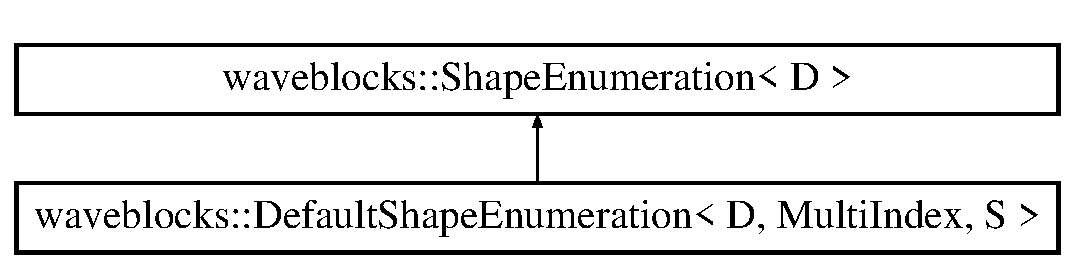
\includegraphics[height=2.000000cm]{classwaveblocks_1_1_default_shape_enumeration}
\end{center}
\end{figure}
\subsection*{Public Member Functions}
\begin{DoxyCompactItemize}
\item 
\hypertarget{classwaveblocks_1_1_default_shape_enumeration_ae1e8c2f51bcd7cf13e39f892e95eddc9}{}{\bfseries Default\+Shape\+Enumeration} (const S \&shape, bool use\+\_\+dict\+\_\+=false)\label{classwaveblocks_1_1_default_shape_enumeration_ae1e8c2f51bcd7cf13e39f892e95eddc9}

\item 
std\+::size\+\_\+t \hyperlink{classwaveblocks_1_1_default_shape_enumeration_aab6571cd94ba28768c569626af5a66a3}{n\+\_\+slices} () const override
\item 
std\+::size\+\_\+t \hyperlink{classwaveblocks_1_1_default_shape_enumeration_a5fc46846d7763190f1911b542bfec103}{size} () const override
\begin{DoxyCompactList}\small\item\em returns number of nodes that are part of the shape \end{DoxyCompactList}\item 
const \hyperlink{classwaveblocks_1_1_shape_slice}{Shape\+Slice}$<$ D $>$ \& \hyperlink{classwaveblocks_1_1_default_shape_enumeration_a323986feed57994f2049627e67cda2cc}{slice} (std\+::size\+\_\+t islice) const override
\item 
bool \hyperlink{classwaveblocks_1_1_default_shape_enumeration_a766b764e141186034ed942b25248f31a}{contains} (const std\+::array$<$ int, D $>$ \&index) const override
\item 
int \hyperlink{classwaveblocks_1_1_default_shape_enumeration_a6b6991c193523c2b66870c65c837b9e6}{bbox} (dim\+\_\+t axis) const override
\begin{DoxyCompactList}\small\item\em retrieves the index of the outmost node in a given axis \end{DoxyCompactList}\end{DoxyCompactItemize}


\subsection{Member Function Documentation}
\hypertarget{classwaveblocks_1_1_default_shape_enumeration_a6b6991c193523c2b66870c65c837b9e6}{}\index{waveblocks\+::\+Default\+Shape\+Enumeration@{waveblocks\+::\+Default\+Shape\+Enumeration}!bbox@{bbox}}
\index{bbox@{bbox}!waveblocks\+::\+Default\+Shape\+Enumeration@{waveblocks\+::\+Default\+Shape\+Enumeration}}
\subsubsection[{bbox}]{\setlength{\rightskip}{0pt plus 5cm}template$<$dim\+\_\+t D, class Multi\+Index , class S $>$ int {\bf waveblocks\+::\+Default\+Shape\+Enumeration}$<$ D, Multi\+Index, S $>$\+::bbox (
\begin{DoxyParamCaption}
\item[{dim\+\_\+t}]{axis}
\end{DoxyParamCaption}
) const\hspace{0.3cm}{\ttfamily [inline]}, {\ttfamily [override]}, {\ttfamily [virtual]}}\label{classwaveblocks_1_1_default_shape_enumeration_a6b6991c193523c2b66870c65c837b9e6}


retrieves the index of the outmost node in a given axis 

\begin{DoxyReturn}{Returns}

\end{DoxyReturn}


Implements \hyperlink{classwaveblocks_1_1_shape_enumeration_a35eb99f86fca58c2983cf8b00432e8c2}{waveblocks\+::\+Shape\+Enumeration$<$ D $>$}.

\hypertarget{classwaveblocks_1_1_default_shape_enumeration_a766b764e141186034ed942b25248f31a}{}\index{waveblocks\+::\+Default\+Shape\+Enumeration@{waveblocks\+::\+Default\+Shape\+Enumeration}!contains@{contains}}
\index{contains@{contains}!waveblocks\+::\+Default\+Shape\+Enumeration@{waveblocks\+::\+Default\+Shape\+Enumeration}}
\subsubsection[{contains}]{\setlength{\rightskip}{0pt plus 5cm}template$<$dim\+\_\+t D, class Multi\+Index , class S $>$ bool {\bf waveblocks\+::\+Default\+Shape\+Enumeration}$<$ D, Multi\+Index, S $>$\+::contains (
\begin{DoxyParamCaption}
\item[{const std\+::array$<$ int, D $>$ \&}]{index}
\end{DoxyParamCaption}
) const\hspace{0.3cm}{\ttfamily [inline]}, {\ttfamily [override]}, {\ttfamily [virtual]}}\label{classwaveblocks_1_1_default_shape_enumeration_a766b764e141186034ed942b25248f31a}
\begin{DoxyReturn}{Returns}
forwards 
\end{DoxyReturn}


Implements \hyperlink{classwaveblocks_1_1_shape_enumeration_af34f5d866923c3f4efc16dec49b4748d}{waveblocks\+::\+Shape\+Enumeration$<$ D $>$}.

\hypertarget{classwaveblocks_1_1_default_shape_enumeration_aab6571cd94ba28768c569626af5a66a3}{}\index{waveblocks\+::\+Default\+Shape\+Enumeration@{waveblocks\+::\+Default\+Shape\+Enumeration}!n\+\_\+slices@{n\+\_\+slices}}
\index{n\+\_\+slices@{n\+\_\+slices}!waveblocks\+::\+Default\+Shape\+Enumeration@{waveblocks\+::\+Default\+Shape\+Enumeration}}
\subsubsection[{n\+\_\+slices}]{\setlength{\rightskip}{0pt plus 5cm}template$<$dim\+\_\+t D, class Multi\+Index , class S $>$ std\+::size\+\_\+t {\bf waveblocks\+::\+Default\+Shape\+Enumeration}$<$ D, Multi\+Index, S $>$\+::n\+\_\+slices (
\begin{DoxyParamCaption}
{}
\end{DoxyParamCaption}
) const\hspace{0.3cm}{\ttfamily [inline]}, {\ttfamily [override]}, {\ttfamily [virtual]}}\label{classwaveblocks_1_1_default_shape_enumeration_aab6571cd94ba28768c569626af5a66a3}
\begin{DoxyReturn}{Returns}
number of (ideally non-\/empty) slices 
\end{DoxyReturn}


Implements \hyperlink{classwaveblocks_1_1_shape_enumeration_a6400c5e4f36b8077b253a18e91d07fb4}{waveblocks\+::\+Shape\+Enumeration$<$ D $>$}.

\hypertarget{classwaveblocks_1_1_default_shape_enumeration_a5fc46846d7763190f1911b542bfec103}{}\index{waveblocks\+::\+Default\+Shape\+Enumeration@{waveblocks\+::\+Default\+Shape\+Enumeration}!size@{size}}
\index{size@{size}!waveblocks\+::\+Default\+Shape\+Enumeration@{waveblocks\+::\+Default\+Shape\+Enumeration}}
\subsubsection[{size}]{\setlength{\rightskip}{0pt plus 5cm}template$<$dim\+\_\+t D, class Multi\+Index , class S $>$ std\+::size\+\_\+t {\bf waveblocks\+::\+Default\+Shape\+Enumeration}$<$ D, Multi\+Index, S $>$\+::size (
\begin{DoxyParamCaption}
{}
\end{DoxyParamCaption}
) const\hspace{0.3cm}{\ttfamily [inline]}, {\ttfamily [override]}, {\ttfamily [virtual]}}\label{classwaveblocks_1_1_default_shape_enumeration_a5fc46846d7763190f1911b542bfec103}


returns number of nodes that are part of the shape 

\begin{DoxyReturn}{Returns}
number of nodes 
\end{DoxyReturn}


Reimplemented from \hyperlink{classwaveblocks_1_1_shape_enumeration_aa40d5659e3c109d8c77144208a9e1c2c}{waveblocks\+::\+Shape\+Enumeration$<$ D $>$}.

\hypertarget{classwaveblocks_1_1_default_shape_enumeration_a323986feed57994f2049627e67cda2cc}{}\index{waveblocks\+::\+Default\+Shape\+Enumeration@{waveblocks\+::\+Default\+Shape\+Enumeration}!slice@{slice}}
\index{slice@{slice}!waveblocks\+::\+Default\+Shape\+Enumeration@{waveblocks\+::\+Default\+Shape\+Enumeration}}
\subsubsection[{slice}]{\setlength{\rightskip}{0pt plus 5cm}template$<$dim\+\_\+t D, class Multi\+Index , class S $>$ const {\bf Shape\+Slice}$<$D$>$\& {\bf waveblocks\+::\+Default\+Shape\+Enumeration}$<$ D, Multi\+Index, S $>$\+::slice (
\begin{DoxyParamCaption}
\item[{std\+::size\+\_\+t}]{islice}
\end{DoxyParamCaption}
) const\hspace{0.3cm}{\ttfamily [inline]}, {\ttfamily [override]}, {\ttfamily [virtual]}}\label{classwaveblocks_1_1_default_shape_enumeration_a323986feed57994f2049627e67cda2cc}

\begin{DoxyParams}[1]{Parameters}
\mbox{\tt in}  & {\em islice} & index of requested slice \\
\hline
\end{DoxyParams}
\begin{DoxyReturn}{Returns}
requested slice or empty slice if (islice $>$= \#slices) 
\end{DoxyReturn}


Implements \hyperlink{classwaveblocks_1_1_shape_enumeration_abb6ab9207b189e4e7b5e67345c4f2ea9}{waveblocks\+::\+Shape\+Enumeration$<$ D $>$}.



The documentation for this class was generated from the following file\+:\begin{DoxyCompactItemize}
\item 
/home/michaja/\+Documents/eth/libwaveblocks/waveblocks/shape\+\_\+enumeration\+\_\+default.\+hpp\end{DoxyCompactItemize}

\hypertarget{classwaveblocks_1_1_default_shape_slice}{}\section{waveblocks\+:\+:Default\+Shape\+Slice$<$ D, Multi\+Index $>$ Class Template Reference}
\label{classwaveblocks_1_1_default_shape_slice}\index{waveblocks\+::\+Default\+Shape\+Slice$<$ D, Multi\+Index $>$@{waveblocks\+::\+Default\+Shape\+Slice$<$ D, Multi\+Index $>$}}


Default implementation of a shape enumeration.  




{\ttfamily \#include $<$shape\+\_\+enumeration\+\_\+default.\+hpp$>$}

Inheritance diagram for waveblocks\+:\+:Default\+Shape\+Slice$<$ D, Multi\+Index $>$\+:\begin{figure}[H]
\begin{center}
\leavevmode
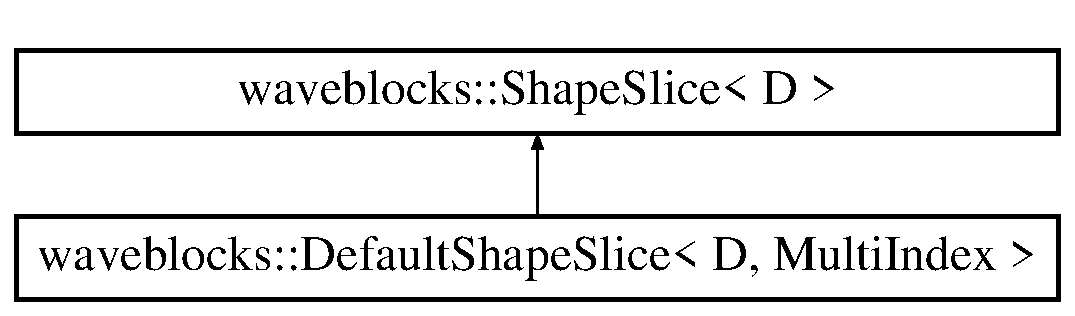
\includegraphics[height=2.000000cm]{classwaveblocks_1_1_default_shape_slice}
\end{center}
\end{figure}
\subsection*{Public Member Functions}
\begin{DoxyCompactItemize}
\item 
std\+::size\+\_\+t \hyperlink{classwaveblocks_1_1_default_shape_slice_aab9cf7a4e321da979afbc6c6b8d27d82}{offset} () const override
\item 
std\+::size\+\_\+t \hyperlink{classwaveblocks_1_1_default_shape_slice_a9e38e466352a0f0023e1fb417be1bf07}{size} () const override
\item 
std\+::size\+\_\+t \hyperlink{classwaveblocks_1_1_default_shape_slice_ad43e2ba8c9f6de8215afe3058f379c29}{slice\+\_\+index} () const override
\item 
std\+::array$<$ int, D $>$ \hyperlink{classwaveblocks_1_1_default_shape_slice_afe08f1250a3e74ec685757b8c5456428}{operator\mbox{[}$\,$\mbox{]}} (std\+::size\+\_\+t ordinal) const override
\begin{DoxyCompactList}\small\item\em Returns the multi-\/index of the node at position {\itshape ordinal}. \end{DoxyCompactList}\item 
std\+::size\+\_\+t \hyperlink{classwaveblocks_1_1_default_shape_slice_ae44dd6209de700b5a370f3815979b883}{find} (const std\+::array$<$ int, D $>$ \&\+\_\+index) const override
\begin{DoxyCompactList}\small\item\em Returns the position of the node with multi-\/index {\ttfamily index}. \end{DoxyCompactList}\item 
virtual std\+::array$<$ std\+::size\+\_\+t, D $>$ \hyperlink{classwaveblocks_1_1_default_shape_slice_a798802b140b441811e9d5ac74b16fb53}{find\+\_\+backward\+\_\+neighbours} (const std\+::array$<$ int, D $>$ \&\+\_\+index) const override
\begin{DoxyCompactList}\small\item\em Retrieves ordinals of all backward neighbours of a given node very efficiently. \end{DoxyCompactList}\end{DoxyCompactItemize}
\subsection*{Friends}
\begin{DoxyCompactItemize}
\item 
\hypertarget{classwaveblocks_1_1_default_shape_slice_a084d0e149c246b1f4005cbae9347ace1}{}{\footnotesize template$<$dim\+\_\+t D\+\_\+, class M\+\_\+ , class S\+\_\+ $>$ }\\class {\bfseries Default\+Shape\+Enumeration}\label{classwaveblocks_1_1_default_shape_slice_a084d0e149c246b1f4005cbae9347ace1}

\end{DoxyCompactItemize}


\subsection{Detailed Description}
\subsubsection*{template$<$dim\+\_\+t D, class Multi\+Index$>$class waveblocks\+::\+Default\+Shape\+Slice$<$ D, Multi\+Index $>$}

Default implementation of a shape enumeration. 

This class takes a shape description object and builds a lookup-\/table to perform queries. It lets the user freely choose an appropriate type to represent multi-\/indices internally.

{\bfseries Implementation details}

This class uses a vector to do {\itshape ordinal -\/$>$ multi-\/index} queries. For {\itshape multi-\/index -\/$>$ ordinal} it does binary search by default. The constructor provides an option to use an hashmap instead. However it turned out that binary search is slightly faster than a hashmap regardless of the hash-\/function.


\begin{DoxyTemplParams}{Template Parameters}
{\em D} & number of multi-\/index dimensions \\
\hline
{\em Multi\+Index} & Type to internally represent a multi-\/index. ~\newline
 A custom type should provide same interface as std\+::array$<$int,\+D$>$. ~\newline
 Furthermore a custom type must specialize std\+::less, std\+::hash, std\+::equal\+\_\+to. \\
\hline
{\em S} & shape description class\\
\hline
\end{DoxyTemplParams}
\begin{DoxySeeAlso}{See also}
\hyperlink{classwaveblocks_1_1_tiny_multi_index}{Tiny\+Multi\+Index} A compressed multi-\/index type that represents all multi-\/indices using a single integer. 
\end{DoxySeeAlso}


\subsection{Member Function Documentation}
\hypertarget{classwaveblocks_1_1_default_shape_slice_ae44dd6209de700b5a370f3815979b883}{}\index{waveblocks\+::\+Default\+Shape\+Slice@{waveblocks\+::\+Default\+Shape\+Slice}!find@{find}}
\index{find@{find}!waveblocks\+::\+Default\+Shape\+Slice@{waveblocks\+::\+Default\+Shape\+Slice}}
\subsubsection[{find}]{\setlength{\rightskip}{0pt plus 5cm}template$<$dim\+\_\+t D, class Multi\+Index $>$ std\+::size\+\_\+t {\bf waveblocks\+::\+Default\+Shape\+Slice}$<$ D, Multi\+Index $>$\+::find (
\begin{DoxyParamCaption}
\item[{const std\+::array$<$ int, D $>$ \&}]{index}
\end{DoxyParamCaption}
) const\hspace{0.3cm}{\ttfamily [inline]}, {\ttfamily [override]}, {\ttfamily [virtual]}}\label{classwaveblocks_1_1_default_shape_slice_ae44dd6209de700b5a370f3815979b883}


Returns the position of the node with multi-\/index {\ttfamily index}. 

Notice that the first node in the slice has position 0 (not 1 or \hyperlink{classwaveblocks_1_1_default_shape_slice_aab9cf7a4e321da979afbc6c6b8d27d82}{offset()}).

Portable programs should never call this function with an node that is not part of this slice since this causes {\itshape undefined} {\itshape behaviour}.

Use Shape\+Enumeration$<$\+D$>$\+::contains(index) to check whether this slice contains the given node.

{\bfseries complexity\+: }logarithmic in the number of slice-\/nodes


\begin{DoxyParams}[1]{Parameters}
\mbox{\tt in}  & {\em index} & multi-\/index of a node in this slice \\
\hline
\end{DoxyParams}
\begin{DoxyReturn}{Returns}
position of the specified node 
\end{DoxyReturn}


Implements \hyperlink{classwaveblocks_1_1_shape_slice_ab38e2bf39cd8d9a2c9a1028622b077b1}{waveblocks\+::\+Shape\+Slice$<$ D $>$}.

\hypertarget{classwaveblocks_1_1_default_shape_slice_a798802b140b441811e9d5ac74b16fb53}{}\index{waveblocks\+::\+Default\+Shape\+Slice@{waveblocks\+::\+Default\+Shape\+Slice}!find\+\_\+backward\+\_\+neighbours@{find\+\_\+backward\+\_\+neighbours}}
\index{find\+\_\+backward\+\_\+neighbours@{find\+\_\+backward\+\_\+neighbours}!waveblocks\+::\+Default\+Shape\+Slice@{waveblocks\+::\+Default\+Shape\+Slice}}
\subsubsection[{find\+\_\+backward\+\_\+neighbours}]{\setlength{\rightskip}{0pt plus 5cm}template$<$dim\+\_\+t D, class Multi\+Index $>$ virtual std\+::array$<$std\+::size\+\_\+t,D$>$ {\bf waveblocks\+::\+Default\+Shape\+Slice}$<$ D, Multi\+Index $>$\+::find\+\_\+backward\+\_\+neighbours (
\begin{DoxyParamCaption}
\item[{const std\+::array$<$ int, D $>$ \&}]{index}
\end{DoxyParamCaption}
) const\hspace{0.3cm}{\ttfamily [inline]}, {\ttfamily [override]}, {\ttfamily [virtual]}}\label{classwaveblocks_1_1_default_shape_slice_a798802b140b441811e9d5ac74b16fb53}


Retrieves ordinals of all backward neighbours of a given node very efficiently. 

Notice that this method assumes that the given node {\bfseries is part of the shape}. Therefore this method does not need to perform any contains()-\/checks since it knows that all backward neighbours exist, except when the given node contains some zero entries. In the latter case, this method returns an undefined ordinal.

If the given node is not part of the shape, then the behaviour is undefined.


\begin{DoxyParams}[1]{Parameters}
\mbox{\tt in}  & {\em index} & node that {\bfseries is part of the shape} \\
\hline
\end{DoxyParams}
\begin{DoxyReturn}{Returns}
For each backward neighbour its ordinal. An ordinal is undefined if its node does not exist. 
\end{DoxyReturn}


Implements \hyperlink{classwaveblocks_1_1_shape_slice_a724b4713602473f6a0b712cf32592ead}{waveblocks\+::\+Shape\+Slice$<$ D $>$}.

\hypertarget{classwaveblocks_1_1_default_shape_slice_aab9cf7a4e321da979afbc6c6b8d27d82}{}\index{waveblocks\+::\+Default\+Shape\+Slice@{waveblocks\+::\+Default\+Shape\+Slice}!offset@{offset}}
\index{offset@{offset}!waveblocks\+::\+Default\+Shape\+Slice@{waveblocks\+::\+Default\+Shape\+Slice}}
\subsubsection[{offset}]{\setlength{\rightskip}{0pt plus 5cm}template$<$dim\+\_\+t D, class Multi\+Index $>$ std\+::size\+\_\+t {\bf waveblocks\+::\+Default\+Shape\+Slice}$<$ D, Multi\+Index $>$\+::offset (
\begin{DoxyParamCaption}
{}
\end{DoxyParamCaption}
) const\hspace{0.3cm}{\ttfamily [inline]}, {\ttfamily [override]}, {\ttfamily [virtual]}}\label{classwaveblocks_1_1_default_shape_slice_aab9cf7a4e321da979afbc6c6b8d27d82}
\begin{DoxyReturn}{Returns}
number of nodes in all previous slices 
\end{DoxyReturn}


Implements \hyperlink{classwaveblocks_1_1_shape_slice_a1304d3ca2c080b8258ddff233c2b1809}{waveblocks\+::\+Shape\+Slice$<$ D $>$}.

\hypertarget{classwaveblocks_1_1_default_shape_slice_afe08f1250a3e74ec685757b8c5456428}{}\index{waveblocks\+::\+Default\+Shape\+Slice@{waveblocks\+::\+Default\+Shape\+Slice}!operator\mbox{[}$\,$\mbox{]}@{operator[]}}
\index{operator\mbox{[}$\,$\mbox{]}@{operator[]}!waveblocks\+::\+Default\+Shape\+Slice@{waveblocks\+::\+Default\+Shape\+Slice}}
\subsubsection[{operator[]}]{\setlength{\rightskip}{0pt plus 5cm}template$<$dim\+\_\+t D, class Multi\+Index $>$ std\+::array$<$int,D$>$ {\bf waveblocks\+::\+Default\+Shape\+Slice}$<$ D, Multi\+Index $>$\+::operator\mbox{[}$\,$\mbox{]} (
\begin{DoxyParamCaption}
\item[{std\+::size\+\_\+t}]{ordinal}
\end{DoxyParamCaption}
) const\hspace{0.3cm}{\ttfamily [inline]}, {\ttfamily [override]}, {\ttfamily [virtual]}}\label{classwaveblocks_1_1_default_shape_slice_afe08f1250a3e74ec685757b8c5456428}


Returns the multi-\/index of the node at position {\itshape ordinal}. 

Notice that the first node in the slice has ordinal 0 (not 1 or \hyperlink{classwaveblocks_1_1_default_shape_slice_aab9cf7a4e321da979afbc6c6b8d27d82}{offset()}).

Portable programs should never call this function with an argument that is {\itshape out-\/of-\/range}, since this causes {\itshape undefined} {\itshape behaviour}.

{\bfseries complexity\+: }logarithmic in the number of slice-\/nodes


\begin{DoxyParams}[1]{Parameters}
\mbox{\tt in}  & {\em ordinal} & position of a node in this slice \\
\hline
\end{DoxyParams}
\begin{DoxyReturn}{Returns}
multi-\/index of the specified node 
\end{DoxyReturn}


Implements \hyperlink{classwaveblocks_1_1_shape_slice_a1e7363a71777b680cafe370ea4be2fb1}{waveblocks\+::\+Shape\+Slice$<$ D $>$}.

\hypertarget{classwaveblocks_1_1_default_shape_slice_a9e38e466352a0f0023e1fb417be1bf07}{}\index{waveblocks\+::\+Default\+Shape\+Slice@{waveblocks\+::\+Default\+Shape\+Slice}!size@{size}}
\index{size@{size}!waveblocks\+::\+Default\+Shape\+Slice@{waveblocks\+::\+Default\+Shape\+Slice}}
\subsubsection[{size}]{\setlength{\rightskip}{0pt plus 5cm}template$<$dim\+\_\+t D, class Multi\+Index $>$ std\+::size\+\_\+t {\bf waveblocks\+::\+Default\+Shape\+Slice}$<$ D, Multi\+Index $>$\+::size (
\begin{DoxyParamCaption}
{}
\end{DoxyParamCaption}
) const\hspace{0.3cm}{\ttfamily [inline]}, {\ttfamily [override]}, {\ttfamily [virtual]}}\label{classwaveblocks_1_1_default_shape_slice_a9e38e466352a0f0023e1fb417be1bf07}
\begin{DoxyReturn}{Returns}
number of nodes in this slice 
\end{DoxyReturn}


Implements \hyperlink{classwaveblocks_1_1_shape_slice_a08b3fd43798dea6e4487e4b41d926f30}{waveblocks\+::\+Shape\+Slice$<$ D $>$}.

\hypertarget{classwaveblocks_1_1_default_shape_slice_ad43e2ba8c9f6de8215afe3058f379c29}{}\index{waveblocks\+::\+Default\+Shape\+Slice@{waveblocks\+::\+Default\+Shape\+Slice}!slice\+\_\+index@{slice\+\_\+index}}
\index{slice\+\_\+index@{slice\+\_\+index}!waveblocks\+::\+Default\+Shape\+Slice@{waveblocks\+::\+Default\+Shape\+Slice}}
\subsubsection[{slice\+\_\+index}]{\setlength{\rightskip}{0pt plus 5cm}template$<$dim\+\_\+t D, class Multi\+Index $>$ std\+::size\+\_\+t {\bf waveblocks\+::\+Default\+Shape\+Slice}$<$ D, Multi\+Index $>$\+::slice\+\_\+index (
\begin{DoxyParamCaption}
{}
\end{DoxyParamCaption}
) const\hspace{0.3cm}{\ttfamily [inline]}, {\ttfamily [override]}, {\ttfamily [virtual]}}\label{classwaveblocks_1_1_default_shape_slice_ad43e2ba8c9f6de8215afe3058f379c29}
\begin{DoxyReturn}{Returns}
index/ordinal of this slice 
\end{DoxyReturn}


Implements \hyperlink{classwaveblocks_1_1_shape_slice_aba345671b0dd4058d4b5de285d904689}{waveblocks\+::\+Shape\+Slice$<$ D $>$}.



The documentation for this class was generated from the following file\+:\begin{DoxyCompactItemize}
\item 
/home/michaja/\+Documents/eth/libwaveblocks/waveblocks/shape\+\_\+enumeration\+\_\+default.\+hpp\end{DoxyCompactItemize}

\hypertarget{classwaveblocks_1_1_tiny_multi_index_1_1_entry}{}\section{waveblocks\+:\+:Tiny\+Multi\+Index$<$ U\+I\+N\+T, D $>$\+:\+:Entry Class Reference}
\label{classwaveblocks_1_1_tiny_multi_index_1_1_entry}\index{waveblocks\+::\+Tiny\+Multi\+Index$<$ U\+I\+N\+T, D $>$\+::\+Entry@{waveblocks\+::\+Tiny\+Multi\+Index$<$ U\+I\+N\+T, D $>$\+::\+Entry}}
\subsection*{Public Member Functions}
\begin{DoxyCompactItemize}
\item 
\hypertarget{classwaveblocks_1_1_tiny_multi_index_1_1_entry_a002a54caf8cfe40a273f57c1859bf70b}{}{\bfseries Entry} (U\+I\+N\+T \&values, std\+::size\+\_\+t index)\label{classwaveblocks_1_1_tiny_multi_index_1_1_entry_a002a54caf8cfe40a273f57c1859bf70b}

\item 
\hypertarget{classwaveblocks_1_1_tiny_multi_index_1_1_entry_a6257e0f2542f2f22faad22ceee5f91a2}{}\hyperlink{classwaveblocks_1_1_tiny_multi_index_1_1_entry}{Entry} \& {\bfseries operator=} (int value)\label{classwaveblocks_1_1_tiny_multi_index_1_1_entry_a6257e0f2542f2f22faad22ceee5f91a2}

\item 
\hypertarget{classwaveblocks_1_1_tiny_multi_index_1_1_entry_a2b6a861952333c67c60f5a991a5fa025}{}\hyperlink{classwaveblocks_1_1_tiny_multi_index_1_1_entry}{Entry} \& {\bfseries operator=} (const \hyperlink{classwaveblocks_1_1_tiny_multi_index_1_1_entry}{Entry} \&entry)\label{classwaveblocks_1_1_tiny_multi_index_1_1_entry_a2b6a861952333c67c60f5a991a5fa025}

\item 
\hypertarget{classwaveblocks_1_1_tiny_multi_index_1_1_entry_ae154508fcec07e28ed6b2264762e3a9f}{}\hyperlink{classwaveblocks_1_1_tiny_multi_index_1_1_entry}{Entry} \& {\bfseries operator+=} (int value)\label{classwaveblocks_1_1_tiny_multi_index_1_1_entry_ae154508fcec07e28ed6b2264762e3a9f}

\item 
\hypertarget{classwaveblocks_1_1_tiny_multi_index_1_1_entry_a40fe0314c9b5436f8ff0ec61fefbd91b}{}\hyperlink{classwaveblocks_1_1_tiny_multi_index_1_1_entry}{Entry} \& {\bfseries operator-\/=} (int value)\label{classwaveblocks_1_1_tiny_multi_index_1_1_entry_a40fe0314c9b5436f8ff0ec61fefbd91b}

\item 
\hypertarget{classwaveblocks_1_1_tiny_multi_index_1_1_entry_a91a1de9c061a29eea2e8677a2f25cb54}{}\hyperlink{classwaveblocks_1_1_tiny_multi_index_1_1_entry}{Entry} \& {\bfseries operator$\ast$=} (int value)\label{classwaveblocks_1_1_tiny_multi_index_1_1_entry_a91a1de9c061a29eea2e8677a2f25cb54}

\item 
\hypertarget{classwaveblocks_1_1_tiny_multi_index_1_1_entry_a14ca00a0a571386267acc2489c7db6c8}{}\hyperlink{classwaveblocks_1_1_tiny_multi_index_1_1_entry}{Entry} \& {\bfseries operator/=} (int value)\label{classwaveblocks_1_1_tiny_multi_index_1_1_entry_a14ca00a0a571386267acc2489c7db6c8}

\item 
\hypertarget{classwaveblocks_1_1_tiny_multi_index_1_1_entry_a7b23682ebb52f09092255e8465e9e250}{}\hyperlink{classwaveblocks_1_1_tiny_multi_index_1_1_entry}{Entry} \& {\bfseries operator\%=} (int value)\label{classwaveblocks_1_1_tiny_multi_index_1_1_entry_a7b23682ebb52f09092255e8465e9e250}

\item 
\hypertarget{classwaveblocks_1_1_tiny_multi_index_1_1_entry_a56d7e2587062a5899875ae9e792cf4c0}{}{\bfseries operator int} () const \label{classwaveblocks_1_1_tiny_multi_index_1_1_entry_a56d7e2587062a5899875ae9e792cf4c0}

\end{DoxyCompactItemize}


The documentation for this class was generated from the following file\+:\begin{DoxyCompactItemize}
\item 
/home/michaja/\+Documents/eth/libwaveblocks/waveblocks/tiny\+\_\+multi\+\_\+index.\+hpp\end{DoxyCompactItemize}

\hypertarget{structstd_1_1equal__to_3_01waveblocks_1_1_tiny_multi_index_3_01_u_i_n_t_00_01_d_01_4_01_4}{}\section{std\+:\+:equal\+\_\+to$<$ waveblocks\+:\+:Tiny\+Multi\+Index$<$ U\+I\+N\+T, D $>$ $>$ Struct Template Reference}
\label{structstd_1_1equal__to_3_01waveblocks_1_1_tiny_multi_index_3_01_u_i_n_t_00_01_d_01_4_01_4}\index{std\+::equal\+\_\+to$<$ waveblocks\+::\+Tiny\+Multi\+Index$<$ U\+I\+N\+T, D $>$ $>$@{std\+::equal\+\_\+to$<$ waveblocks\+::\+Tiny\+Multi\+Index$<$ U\+I\+N\+T, D $>$ $>$}}


{\ttfamily \#include $<$tiny\+\_\+multi\+\_\+index.\+hpp$>$}

\subsection*{Public Types}
\begin{DoxyCompactItemize}
\item 
\hypertarget{structstd_1_1equal__to_3_01waveblocks_1_1_tiny_multi_index_3_01_u_i_n_t_00_01_d_01_4_01_4_a09a4eb594dc696b06ad4309a1f6fe963}{}typedef \hyperlink{classwaveblocks_1_1_tiny_multi_index}{Multi\+Index} {\bfseries first\+\_\+argument\+\_\+type}\label{structstd_1_1equal__to_3_01waveblocks_1_1_tiny_multi_index_3_01_u_i_n_t_00_01_d_01_4_01_4_a09a4eb594dc696b06ad4309a1f6fe963}

\item 
\hypertarget{structstd_1_1equal__to_3_01waveblocks_1_1_tiny_multi_index_3_01_u_i_n_t_00_01_d_01_4_01_4_a9118414cd5c1cd6ca52fcfbaf7945cc8}{}typedef \hyperlink{classwaveblocks_1_1_tiny_multi_index}{Multi\+Index} {\bfseries second\+\_\+argument\+\_\+type}\label{structstd_1_1equal__to_3_01waveblocks_1_1_tiny_multi_index_3_01_u_i_n_t_00_01_d_01_4_01_4_a9118414cd5c1cd6ca52fcfbaf7945cc8}

\item 
\hypertarget{structstd_1_1equal__to_3_01waveblocks_1_1_tiny_multi_index_3_01_u_i_n_t_00_01_d_01_4_01_4_a65ab526d6a5449430c0f6aca169b58f9}{}typedef bool {\bfseries result\+\_\+type}\label{structstd_1_1equal__to_3_01waveblocks_1_1_tiny_multi_index_3_01_u_i_n_t_00_01_d_01_4_01_4_a65ab526d6a5449430c0f6aca169b58f9}

\end{DoxyCompactItemize}
\subsection*{Public Member Functions}
\begin{DoxyCompactItemize}
\item 
\hypertarget{structstd_1_1equal__to_3_01waveblocks_1_1_tiny_multi_index_3_01_u_i_n_t_00_01_d_01_4_01_4_a75a16199830e2f494b8b4ba127c011c3}{}bool {\bfseries operator()} (const \hyperlink{classwaveblocks_1_1_tiny_multi_index}{Multi\+Index} \&first, const \hyperlink{classwaveblocks_1_1_tiny_multi_index}{Multi\+Index} \&second) const \label{structstd_1_1equal__to_3_01waveblocks_1_1_tiny_multi_index_3_01_u_i_n_t_00_01_d_01_4_01_4_a75a16199830e2f494b8b4ba127c011c3}

\end{DoxyCompactItemize}


\subsection{Detailed Description}
\subsubsection*{template$<$class U\+I\+N\+T, waveblocks\+::dim\+\_\+t D$>$struct std\+::equal\+\_\+to$<$ waveblocks\+::\+Tiny\+Multi\+Index$<$ U\+I\+N\+T, D $>$ $>$}

provides equality functor for S\+T\+L (notable std\+::unordered\+\_\+map) specializes generic std\+::equal\+\_\+to$<$\+T$>$ 

The documentation for this struct was generated from the following file\+:\begin{DoxyCompactItemize}
\item 
/home/michaja/\+Documents/eth/libwaveblocks/waveblocks/tiny\+\_\+multi\+\_\+index.\+hpp\end{DoxyCompactItemize}

\hypertarget{classwaveblocks_1_1_evaluator}{}\section{waveblocks\+:\+:Evaluator$<$ D, N $>$ Class Template Reference}
\label{classwaveblocks_1_1_evaluator}\index{waveblocks\+::\+Evaluator$<$ D, N $>$@{waveblocks\+::\+Evaluator$<$ D, N $>$}}


{\ttfamily \#include $<$hagedorn\+\_\+basis\+\_\+evaluator.\+hpp$>$}

\subsection*{Public Types}
\begin{DoxyCompactItemize}
\item 
typedef Eigen\+::\+Matrix$<$ complex\+\_\+t, D, D $>$ \hyperlink{classwaveblocks_1_1_evaluator_a09bb8abec377b4651699c52d02447ad5}{C\+Matrix\+D\+D}
\item 
typedef Eigen\+::\+Array$<$ complex\+\_\+t, 1, N $>$ \hyperlink{classwaveblocks_1_1_evaluator_a49231d0afba65ca701dfdfb9f3c44c14}{C\+Array1\+N}
\item 
typedef Eigen\+::\+Matrix$<$ complex\+\_\+t, D, N $>$ \hyperlink{classwaveblocks_1_1_evaluator_ac9f759ecd07665903ed76d82ac68dc9a}{C\+Matrix\+D\+N}
\item 
\hypertarget{classwaveblocks_1_1_evaluator_aca0e8511e161fc288509f5cf7eeab0af}{}typedef Eigen\+::\+Matrix$<$ real\+\_\+t, D, N $>$ {\bfseries R\+Matrix\+D\+N}\label{classwaveblocks_1_1_evaluator_aca0e8511e161fc288509f5cf7eeab0af}

\item 
typedef Eigen\+::\+Array$<$ complex\+\_\+t, Eigen\+::\+Dynamic, N $>$ \hyperlink{classwaveblocks_1_1_evaluator_ae67334d6256ba6054f452a15d36c4941}{C\+Array\+X\+N}
\end{DoxyCompactItemize}
\subsection*{Public Member Functions}
\begin{DoxyCompactItemize}
\item 
\hypertarget{classwaveblocks_1_1_evaluator_a2995a06e1a3e9ee459f2ed2186044933}{}{\bfseries Evaluator} (real\+\_\+t eps, std\+::shared\+\_\+ptr$<$ \hyperlink{structwaveblocks_1_1_hagedorn_parameter_set}{Hagedorn\+Parameter\+Set}$<$ D $>$ $>$ parameters, std\+::shared\+\_\+ptr$<$ \hyperlink{classwaveblocks_1_1_shape_enumeration}{Shape\+Enumeration}$<$ D $>$ $>$ enumeration, const \hyperlink{classwaveblocks_1_1_evaluator_ac9f759ecd07665903ed76d82ac68dc9a}{C\+Matrix\+D\+N} \&x)\label{classwaveblocks_1_1_evaluator_a2995a06e1a3e9ee459f2ed2186044933}

\item 
\hyperlink{classwaveblocks_1_1_evaluator_a49231d0afba65ca701dfdfb9f3c44c14}{C\+Array1\+N} \hyperlink{classwaveblocks_1_1_evaluator_a54a68a67c04f3c30e41687572e73998b}{seed} () const 
\begin{DoxyCompactList}\small\item\em Evaluates value of the basis function with multi-\/index (0,0,...,0) \end{DoxyCompactList}\item 
\hyperlink{classwaveblocks_1_1_evaluator_ae67334d6256ba6054f452a15d36c4941}{C\+Array\+X\+N} \hyperlink{classwaveblocks_1_1_evaluator_ae5070ca7d51cc6a28d8e3eeba3d6ddaf}{step} (std\+::size\+\_\+t islice, const \hyperlink{classwaveblocks_1_1_evaluator_ae67334d6256ba6054f452a15d36c4941}{C\+Array\+X\+N} \&prev\+\_\+basis, const \hyperlink{classwaveblocks_1_1_evaluator_ae67334d6256ba6054f452a15d36c4941}{C\+Array\+X\+N} \&curr\+\_\+basis) const 
\end{DoxyCompactItemize}


\subsection{Detailed Description}
\subsubsection*{template$<$dim\+\_\+t D, int N$>$class waveblocks\+::\+Evaluator$<$ D, N $>$}


\begin{DoxyTemplParams}{Template Parameters}
{\em N} & number of quadrature points (if unknown\+: use Eigen\+::\+Dynamic) \\
\hline
\end{DoxyTemplParams}


\subsection{Member Typedef Documentation}
\hypertarget{classwaveblocks_1_1_evaluator_a49231d0afba65ca701dfdfb9f3c44c14}{}\index{waveblocks\+::\+Evaluator@{waveblocks\+::\+Evaluator}!C\+Array1\+N@{C\+Array1\+N}}
\index{C\+Array1\+N@{C\+Array1\+N}!waveblocks\+::\+Evaluator@{waveblocks\+::\+Evaluator}}
\subsubsection[{C\+Array1\+N}]{\setlength{\rightskip}{0pt plus 5cm}template$<$dim\+\_\+t D, int N$>$ typedef Eigen\+::\+Array$<$complex\+\_\+t,1,N$>$ {\bf waveblocks\+::\+Evaluator}$<$ D, N $>$\+::{\bf C\+Array1\+N}}\label{classwaveblocks_1_1_evaluator_a49231d0afba65ca701dfdfb9f3c44c14}
array size\+: (1, \#quadrature points) \hypertarget{classwaveblocks_1_1_evaluator_ae67334d6256ba6054f452a15d36c4941}{}\index{waveblocks\+::\+Evaluator@{waveblocks\+::\+Evaluator}!C\+Array\+X\+N@{C\+Array\+X\+N}}
\index{C\+Array\+X\+N@{C\+Array\+X\+N}!waveblocks\+::\+Evaluator@{waveblocks\+::\+Evaluator}}
\subsubsection[{C\+Array\+X\+N}]{\setlength{\rightskip}{0pt plus 5cm}template$<$dim\+\_\+t D, int N$>$ typedef Eigen\+::\+Array$<$complex\+\_\+t,Eigen\+::\+Dynamic,N$>$ {\bf waveblocks\+::\+Evaluator}$<$ D, N $>$\+::{\bf C\+Array\+X\+N}}\label{classwaveblocks_1_1_evaluator_ae67334d6256ba6054f452a15d36c4941}
matrix size\+: (/unspecified/, \#quadrature points) \hypertarget{classwaveblocks_1_1_evaluator_a09bb8abec377b4651699c52d02447ad5}{}\index{waveblocks\+::\+Evaluator@{waveblocks\+::\+Evaluator}!C\+Matrix\+D\+D@{C\+Matrix\+D\+D}}
\index{C\+Matrix\+D\+D@{C\+Matrix\+D\+D}!waveblocks\+::\+Evaluator@{waveblocks\+::\+Evaluator}}
\subsubsection[{C\+Matrix\+D\+D}]{\setlength{\rightskip}{0pt plus 5cm}template$<$dim\+\_\+t D, int N$>$ typedef Eigen\+::\+Matrix$<$complex\+\_\+t,D,D$>$ {\bf waveblocks\+::\+Evaluator}$<$ D, N $>$\+::{\bf C\+Matrix\+D\+D}}\label{classwaveblocks_1_1_evaluator_a09bb8abec377b4651699c52d02447ad5}
complex square matrix size\+: (\#dimensions) \hypertarget{classwaveblocks_1_1_evaluator_ac9f759ecd07665903ed76d82ac68dc9a}{}\index{waveblocks\+::\+Evaluator@{waveblocks\+::\+Evaluator}!C\+Matrix\+D\+N@{C\+Matrix\+D\+N}}
\index{C\+Matrix\+D\+N@{C\+Matrix\+D\+N}!waveblocks\+::\+Evaluator@{waveblocks\+::\+Evaluator}}
\subsubsection[{C\+Matrix\+D\+N}]{\setlength{\rightskip}{0pt plus 5cm}template$<$dim\+\_\+t D, int N$>$ typedef Eigen\+::\+Matrix$<$complex\+\_\+t,D,N$>$ {\bf waveblocks\+::\+Evaluator}$<$ D, N $>$\+::{\bf C\+Matrix\+D\+N}}\label{classwaveblocks_1_1_evaluator_ac9f759ecd07665903ed76d82ac68dc9a}
matrix size\+: (\#dimensions, \#quadrature points) 

\subsection{Member Function Documentation}
\hypertarget{classwaveblocks_1_1_evaluator_a54a68a67c04f3c30e41687572e73998b}{}\index{waveblocks\+::\+Evaluator@{waveblocks\+::\+Evaluator}!seed@{seed}}
\index{seed@{seed}!waveblocks\+::\+Evaluator@{waveblocks\+::\+Evaluator}}
\subsubsection[{seed}]{\setlength{\rightskip}{0pt plus 5cm}template$<$dim\+\_\+t D, int N$>$ {\bf C\+Array1\+N} {\bf waveblocks\+::\+Evaluator}$<$ D, N $>$\+::seed (
\begin{DoxyParamCaption}
{}
\end{DoxyParamCaption}
) const\hspace{0.3cm}{\ttfamily [inline]}}\label{classwaveblocks_1_1_evaluator_a54a68a67c04f3c30e41687572e73998b}


Evaluates value of the basis function with multi-\/index (0,0,...,0) 

\begin{DoxyReturn}{Returns}
(1,N)-\/\+Matrix 
\end{DoxyReturn}
\hypertarget{classwaveblocks_1_1_evaluator_ae5070ca7d51cc6a28d8e3eeba3d6ddaf}{}\index{waveblocks\+::\+Evaluator@{waveblocks\+::\+Evaluator}!step@{step}}
\index{step@{step}!waveblocks\+::\+Evaluator@{waveblocks\+::\+Evaluator}}
\subsubsection[{step}]{\setlength{\rightskip}{0pt plus 5cm}template$<$dim\+\_\+t D, int N$>$ {\bf C\+Array\+X\+N} {\bf waveblocks\+::\+Evaluator}$<$ D, N $>$\+::step (
\begin{DoxyParamCaption}
\item[{std\+::size\+\_\+t}]{islice, }
\item[{const {\bf C\+Array\+X\+N} \&}]{prev\+\_\+basis, }
\item[{const {\bf C\+Array\+X\+N} \&}]{curr\+\_\+basis}
\end{DoxyParamCaption}
) const\hspace{0.3cm}{\ttfamily [inline]}}\label{classwaveblocks_1_1_evaluator_ae5070ca7d51cc6a28d8e3eeba3d6ddaf}

\begin{DoxyParams}[1]{Parameters}
\mbox{\tt in}  & {\em islice} & ordinal of current slice \\
\hline
\mbox{\tt in}  & {\em prev\+\_\+basis} & basis values of previous slice \\
\hline
\mbox{\tt in}  & {\em curr\+\_\+basis} & basis values of current slice \\
\hline
\end{DoxyParams}
\begin{DoxyReturn}{Returns}
computed basis values of next slice 
\end{DoxyReturn}


The documentation for this class was generated from the following file\+:\begin{DoxyCompactItemize}
\item 
/home/michaja/\+Documents/eth/libwaveblocks/waveblocks/hagedorn\+\_\+basis\+\_\+evaluator.\+hpp\end{DoxyCompactItemize}

\hypertarget{classwaveblocks_1_1_extended_shape}{}\section{waveblocks\+:\+:Extended\+Shape$<$ D, S $>$ Class Template Reference}
\label{classwaveblocks_1_1_extended_shape}\index{waveblocks\+::\+Extended\+Shape$<$ D, S $>$@{waveblocks\+::\+Extended\+Shape$<$ D, S $>$}}
\subsection*{Public Member Functions}
\begin{DoxyCompactItemize}
\item 
\hypertarget{classwaveblocks_1_1_extended_shape_a6ad7be5029d1bfc38a0a1d896a750fd8}{}{\bfseries Extended\+Shape} (S shape)\label{classwaveblocks_1_1_extended_shape_a6ad7be5029d1bfc38a0a1d896a750fd8}

\item 
\hypertarget{classwaveblocks_1_1_extended_shape_a57ce726fd86c72f83a599ad9d9cd9386}{}int {\bfseries bbox} (dim\+\_\+t axis) const \label{classwaveblocks_1_1_extended_shape_a57ce726fd86c72f83a599ad9d9cd9386}

\item 
\hypertarget{classwaveblocks_1_1_extended_shape_a3173c2e80bccb101e23006c9697e2e51}{}{\footnotesize template$<$class Multi\+Index $>$ }\\int {\bfseries limit} (const Multi\+Index \&index, dim\+\_\+t axis) const \label{classwaveblocks_1_1_extended_shape_a3173c2e80bccb101e23006c9697e2e51}

\item 
\hypertarget{classwaveblocks_1_1_extended_shape_ae7de867b655d28453405533f90824a9e}{}std\+::string {\bfseries description} () const \label{classwaveblocks_1_1_extended_shape_ae7de867b655d28453405533f90824a9e}

\end{DoxyCompactItemize}


The documentation for this class was generated from the following file\+:\begin{DoxyCompactItemize}
\item 
/home/michaja/\+Documents/eth/libwaveblocks/waveblocks/shape\+\_\+extended.\+hpp\end{DoxyCompactItemize}

\hypertarget{classwaveblocks_1_1_extended_shape_3_01_d_00_01_hyper_cubic_shape_3_01_d_01_4_01_4}{}\section{waveblocks\+:\+:Extended\+Shape$<$ D, Hyper\+Cubic\+Shape$<$ D $>$ $>$ Class Template Reference}
\label{classwaveblocks_1_1_extended_shape_3_01_d_00_01_hyper_cubic_shape_3_01_d_01_4_01_4}\index{waveblocks\+::\+Extended\+Shape$<$ D, Hyper\+Cubic\+Shape$<$ D $>$ $>$@{waveblocks\+::\+Extended\+Shape$<$ D, Hyper\+Cubic\+Shape$<$ D $>$ $>$}}
\subsection*{Public Member Functions}
\begin{DoxyCompactItemize}
\item 
\hypertarget{classwaveblocks_1_1_extended_shape_3_01_d_00_01_hyper_cubic_shape_3_01_d_01_4_01_4_a48712bbf18a9e12f6b2cf937969c6500}{}{\bfseries Extended\+Shape} (\hyperlink{classwaveblocks_1_1_hyper_cubic_shape}{Hyper\+Cubic\+Shape}$<$ D $>$ shape)\label{classwaveblocks_1_1_extended_shape_3_01_d_00_01_hyper_cubic_shape_3_01_d_01_4_01_4_a48712bbf18a9e12f6b2cf937969c6500}

\item 
\hypertarget{classwaveblocks_1_1_extended_shape_3_01_d_00_01_hyper_cubic_shape_3_01_d_01_4_01_4_a9a766abe6fbb571e0ae0c3502c2161dd}{}int {\bfseries bbox} (dim\+\_\+t axis) const \label{classwaveblocks_1_1_extended_shape_3_01_d_00_01_hyper_cubic_shape_3_01_d_01_4_01_4_a9a766abe6fbb571e0ae0c3502c2161dd}

\item 
\hypertarget{classwaveblocks_1_1_extended_shape_3_01_d_00_01_hyper_cubic_shape_3_01_d_01_4_01_4_a18e1f2b340150d1f866f5231d2eadeb0}{}{\footnotesize template$<$class Multi\+Index $>$ }\\int {\bfseries limit} (const Multi\+Index \&index, dim\+\_\+t axis) const \label{classwaveblocks_1_1_extended_shape_3_01_d_00_01_hyper_cubic_shape_3_01_d_01_4_01_4_a18e1f2b340150d1f866f5231d2eadeb0}

\item 
\hypertarget{classwaveblocks_1_1_extended_shape_3_01_d_00_01_hyper_cubic_shape_3_01_d_01_4_01_4_ad1074adb7bd3959cd8461e6b607ace04}{}std\+::string {\bfseries description} () const \label{classwaveblocks_1_1_extended_shape_3_01_d_00_01_hyper_cubic_shape_3_01_d_01_4_01_4_ad1074adb7bd3959cd8461e6b607ace04}

\end{DoxyCompactItemize}


The documentation for this class was generated from the following file\+:\begin{DoxyCompactItemize}
\item 
/home/michaja/\+Documents/eth/libwaveblocks/waveblocks/shape\+\_\+extended.\+hpp\end{DoxyCompactItemize}

\hypertarget{classwaveblocks_1_1_gradient_operator}{}\section{waveblocks\+:\+:Gradient\+Operator$<$ D $>$ Class Template Reference}
\label{classwaveblocks_1_1_gradient_operator}\index{waveblocks\+::\+Gradient\+Operator$<$ D $>$@{waveblocks\+::\+Gradient\+Operator$<$ D $>$}}
\subsection*{Public Member Functions}
\begin{DoxyCompactItemize}
\item 
\hypertarget{classwaveblocks_1_1_gradient_operator_a38ca05205656b574dce4c6d99de13428}{}{\bfseries Gradient\+Operator} (const std\+::shared\+\_\+ptr$<$ \hyperlink{classwaveblocks_1_1_shape_enumeration}{Shape\+Enumeration}$<$ D $>$ $>$ \&grad\+\_\+enum)\label{classwaveblocks_1_1_gradient_operator_a38ca05205656b574dce4c6d99de13428}

\item 
\hypertarget{classwaveblocks_1_1_gradient_operator_a14e70fe090030dc57b9b55225fb4ee2f}{}{\bfseries Gradient\+Operator} (const \hyperlink{classwaveblocks_1_1_gradient_operator}{Gradient\+Operator}$<$ D $>$ \&other)=default\label{classwaveblocks_1_1_gradient_operator_a14e70fe090030dc57b9b55225fb4ee2f}

\item 
\hypertarget{classwaveblocks_1_1_gradient_operator_a873a9ee5c453ac5bb426da0b1c16d9aa}{}\hyperlink{classwaveblocks_1_1_gradient_operator}{Gradient\+Operator} \& {\bfseries operator=} (const \hyperlink{classwaveblocks_1_1_gradient_operator}{Gradient\+Operator}$<$ D $>$ \&other)=default\label{classwaveblocks_1_1_gradient_operator_a873a9ee5c453ac5bb426da0b1c16d9aa}

\item 
\hypertarget{classwaveblocks_1_1_gradient_operator_a21e784ff2341dc0d04c51b9bace48f65}{}std\+::array$<$ \hyperlink{classwaveblocks_1_1_hagedorn_wavepacket}{Hagedorn\+Wavepacket}$<$ D $>$, D $>$ {\bfseries operator()} (const \hyperlink{classwaveblocks_1_1_hagedorn_wavepacket}{Hagedorn\+Wavepacket}$<$ D $>$ \&wavepacket) const \label{classwaveblocks_1_1_gradient_operator_a21e784ff2341dc0d04c51b9bace48f65}

\end{DoxyCompactItemize}


The documentation for this class was generated from the following file\+:\begin{DoxyCompactItemize}
\item 
/home/michaja/\+Documents/eth/libwaveblocks/waveblocks/hagedorn\+\_\+gradient\+\_\+operator.\+hpp\end{DoxyCompactItemize}

\hypertarget{classwaveblocks_1_1_hagedorn_basis_vector}{}\section{waveblocks\+:\+:Hagedorn\+Basis\+Vector$<$ D, C $>$ Class Template Reference}
\label{classwaveblocks_1_1_hagedorn_basis_vector}\index{waveblocks\+::\+Hagedorn\+Basis\+Vector$<$ D, C $>$@{waveblocks\+::\+Hagedorn\+Basis\+Vector$<$ D, C $>$}}


{\ttfamily \#include $<$hagedorn\+\_\+basis\+\_\+vector.\+hpp$>$}

\subsection*{Public Member Functions}
\begin{DoxyCompactItemize}
\item 
\hypertarget{classwaveblocks_1_1_hagedorn_basis_vector_a1695e11a7ba9e702a0a08c8654adc531}{}\hyperlink{classwaveblocks_1_1_hagedorn_basis_vector}{Hagedorn\+Basis\+Vector} \& {\bfseries operator=} ()\label{classwaveblocks_1_1_hagedorn_basis_vector_a1695e11a7ba9e702a0a08c8654adc531}

\item 
\hypertarget{classwaveblocks_1_1_hagedorn_basis_vector_a8693a19efb02de313a07ec1062be4401}{}complex\+\_\+t {\bfseries operator\mbox{[}$\,$\mbox{]}} (std\+::size\+\_\+t ordinal) const \label{classwaveblocks_1_1_hagedorn_basis_vector_a8693a19efb02de313a07ec1062be4401}

\end{DoxyCompactItemize}
\subsection*{Public Attributes}
\begin{DoxyCompactItemize}
\item 
\hypertarget{classwaveblocks_1_1_hagedorn_basis_vector_a974eac628768ffaed92ad4d59e0c3414}{}std\+::shared\+\_\+ptr$<$ std\+::vector$<$ complex\+\_\+t $>$ $>$ {\bfseries basis\+\_\+}\label{classwaveblocks_1_1_hagedorn_basis_vector_a974eac628768ffaed92ad4d59e0c3414}

\item 
\hypertarget{classwaveblocks_1_1_hagedorn_basis_vector_a97c749161b09e86d6813d8be86271f53}{}std\+::shared\+\_\+ptr$<$ \hyperlink{classwaveblocks_1_1_shape_enumeration}{Shape\+Enumeration}$<$ D $>$ $>$ {\bfseries enumeration\+\_\+}\label{classwaveblocks_1_1_hagedorn_basis_vector_a97c749161b09e86d6813d8be86271f53}

\end{DoxyCompactItemize}


\subsection{Detailed Description}
\subsubsection*{template$<$dim\+\_\+t D, int C = 1$>$class waveblocks\+::\+Hagedorn\+Basis\+Vector$<$ D, C $>$}


\begin{DoxyTemplParams}{Template Parameters}
{\em D} & dimension of shape \\
\hline
{\em C} & numbers of components if wavepacket is vector-\/valued \\
\hline
\end{DoxyTemplParams}


The documentation for this class was generated from the following file\+:\begin{DoxyCompactItemize}
\item 
/home/michaja/\+Documents/eth/libwaveblocks/waveblocks/hagedorn\+\_\+basis\+\_\+vector.\+hpp\end{DoxyCompactItemize}

\hypertarget{structwaveblocks_1_1_hagedorn_parameter_set}{}\section{waveblocks\+:\+:Hagedorn\+Parameter\+Set$<$ D $>$ Struct Template Reference}
\label{structwaveblocks_1_1_hagedorn_parameter_set}\index{waveblocks\+::\+Hagedorn\+Parameter\+Set$<$ D $>$@{waveblocks\+::\+Hagedorn\+Parameter\+Set$<$ D $>$}}
\subsection*{Public Member Functions}
\begin{DoxyCompactItemize}
\item 
\hypertarget{structwaveblocks_1_1_hagedorn_parameter_set_a6a4093ecc987d07ef1280770cba17ef5}{}{\bfseries Hagedorn\+Parameter\+Set} (const \hyperlink{structwaveblocks_1_1_hagedorn_parameter_set}{Hagedorn\+Parameter\+Set} \&that)\label{structwaveblocks_1_1_hagedorn_parameter_set_a6a4093ecc987d07ef1280770cba17ef5}

\item 
\hypertarget{structwaveblocks_1_1_hagedorn_parameter_set_a942784fab6a0514a8adb9ca474e0180a}{}{\bfseries Hagedorn\+Parameter\+Set} (const R\+Matrix$<$ D, 1 $>$ \&q, const R\+Matrix$<$ D, 1 $>$ \&p, const C\+Matrix$<$ D, D $>$ \&Q, const C\+Matrix$<$ D, D $>$ \&P)\label{structwaveblocks_1_1_hagedorn_parameter_set_a942784fab6a0514a8adb9ca474e0180a}

\item 
\hypertarget{structwaveblocks_1_1_hagedorn_parameter_set_a72196745e44d089170f0dfd3c039a695}{}{\bfseries Hagedorn\+Parameter\+Set} (const R\+Matrix$<$ D, 1 $>$ \&q, const R\+Matrix$<$ D, 1 $>$ \&p, const C\+Matrix$<$ D, D $>$ \&Q, const C\+Matrix$<$ D, D $>$ \&P, \hyperlink{classwaveblocks_1_1_continuous_sqrt}{Continuous\+Sqrt}$<$ real\+\_\+t $>$ sqrt\+\_\+det\+Q)\label{structwaveblocks_1_1_hagedorn_parameter_set_a72196745e44d089170f0dfd3c039a695}

\item 
\hypertarget{structwaveblocks_1_1_hagedorn_parameter_set_a5aced398bf12f24d1ed1a8000ec0c46e}{}\hyperlink{structwaveblocks_1_1_hagedorn_parameter_set}{Hagedorn\+Parameter\+Set} \& {\bfseries operator=} (const \hyperlink{structwaveblocks_1_1_hagedorn_parameter_set}{Hagedorn\+Parameter\+Set} \&that)\label{structwaveblocks_1_1_hagedorn_parameter_set_a5aced398bf12f24d1ed1a8000ec0c46e}

\item 
bool \hyperlink{structwaveblocks_1_1_hagedorn_parameter_set_a5fe480ec9fc245780d9b27a04c89444c}{compatible} () const 
\item 
\hypertarget{structwaveblocks_1_1_hagedorn_parameter_set_a38983ea6b7b773077c2dff06cab377ca}{}std\+::pair$<$ R\+Matrix$<$ D, 1 $>$, R\+Matrix$<$ D, D $>$ $>$ {\bfseries mix} (const \hyperlink{structwaveblocks_1_1_hagedorn_parameter_set}{Hagedorn\+Parameter\+Set}$<$ D $>$ \&other) const \label{structwaveblocks_1_1_hagedorn_parameter_set_a38983ea6b7b773077c2dff06cab377ca}

\end{DoxyCompactItemize}
\subsection*{Public Attributes}
\begin{DoxyCompactItemize}
\item 
\hypertarget{structwaveblocks_1_1_hagedorn_parameter_set_ac52f85f8cd3b952693795e7839f239b6}{}R\+Matrix$<$ D, 1 $>$ {\bfseries q}\label{structwaveblocks_1_1_hagedorn_parameter_set_ac52f85f8cd3b952693795e7839f239b6}

\item 
\hypertarget{structwaveblocks_1_1_hagedorn_parameter_set_afe034c134d41b2d414a4e44bb26a8d26}{}R\+Matrix$<$ D, 1 $>$ {\bfseries p}\label{structwaveblocks_1_1_hagedorn_parameter_set_afe034c134d41b2d414a4e44bb26a8d26}

\item 
\hypertarget{structwaveblocks_1_1_hagedorn_parameter_set_a09140cc30176a49868e4cdf15a76bef0}{}C\+Matrix$<$ D, D $>$ {\bfseries Q}\label{structwaveblocks_1_1_hagedorn_parameter_set_a09140cc30176a49868e4cdf15a76bef0}

\item 
\hypertarget{structwaveblocks_1_1_hagedorn_parameter_set_a1be6c9ee56d10d2411018502526f3f72}{}C\+Matrix$<$ D, D $>$ {\bfseries P}\label{structwaveblocks_1_1_hagedorn_parameter_set_a1be6c9ee56d10d2411018502526f3f72}

\item 
\hypertarget{structwaveblocks_1_1_hagedorn_parameter_set_ab149b2b84bd428a2ceafe0df41831890}{}\hyperlink{classwaveblocks_1_1_continuous_sqrt}{Continuous\+Sqrt}$<$ real\+\_\+t $>$ {\bfseries sqrt\+\_\+det\+Q}\label{structwaveblocks_1_1_hagedorn_parameter_set_ab149b2b84bd428a2ceafe0df41831890}

\end{DoxyCompactItemize}


\subsection{Member Function Documentation}
\hypertarget{structwaveblocks_1_1_hagedorn_parameter_set_a5fe480ec9fc245780d9b27a04c89444c}{}\index{waveblocks\+::\+Hagedorn\+Parameter\+Set@{waveblocks\+::\+Hagedorn\+Parameter\+Set}!compatible@{compatible}}
\index{compatible@{compatible}!waveblocks\+::\+Hagedorn\+Parameter\+Set@{waveblocks\+::\+Hagedorn\+Parameter\+Set}}
\subsubsection[{compatible}]{\setlength{\rightskip}{0pt plus 5cm}template$<$dim\+\_\+t D$>$ bool {\bf waveblocks\+::\+Hagedorn\+Parameter\+Set}$<$ D $>$\+::compatible (
\begin{DoxyParamCaption}
{}
\end{DoxyParamCaption}
) const\hspace{0.3cm}{\ttfamily [inline]}}\label{structwaveblocks_1_1_hagedorn_parameter_set_a5fe480ec9fc245780d9b27a04c89444c}
Checks for compatibility relations For details see master thesis 3.\+11 

The documentation for this struct was generated from the following file\+:\begin{DoxyCompactItemize}
\item 
/home/michaja/\+Documents/eth/libwaveblocks/waveblocks/hagedorn\+\_\+parameter\+\_\+set.\+hpp\end{DoxyCompactItemize}

\hypertarget{classwaveblocks_1_1_hagedorn_wavepacket}{}\section{waveblocks\+:\+:Hagedorn\+Wavepacket$<$ D $>$ Class Template Reference}
\label{classwaveblocks_1_1_hagedorn_wavepacket}\index{waveblocks\+::\+Hagedorn\+Wavepacket$<$ D $>$@{waveblocks\+::\+Hagedorn\+Wavepacket$<$ D $>$}}


{\ttfamily \#include $<$hagedorn\+\_\+wavepacket.\+hpp$>$}

\subsection*{Public Types}
\begin{DoxyCompactItemize}
\item 
\hypertarget{classwaveblocks_1_1_hagedorn_wavepacket_a251e571828b08bafb78b894fa28e9678}{}typedef Eigen\+::\+Matrix$<$ complex\+\_\+t, D, 1 $>$ {\bfseries C\+Matrix\+D1}\label{classwaveblocks_1_1_hagedorn_wavepacket_a251e571828b08bafb78b894fa28e9678}

\item 
\hypertarget{classwaveblocks_1_1_hagedorn_wavepacket_a7a5e41136181dbba286042d153988164}{}typedef Eigen\+::\+Matrix$<$ real\+\_\+t, D, 1 $>$ {\bfseries R\+Matrix\+D1}\label{classwaveblocks_1_1_hagedorn_wavepacket_a7a5e41136181dbba286042d153988164}

\item 
typedef Eigen\+::\+Matrix$<$ complex\+\_\+t, D, D $>$ \hyperlink{classwaveblocks_1_1_hagedorn_wavepacket_af285e57872af93378e2fd77c5ab7f528}{C\+Matrix\+D\+D}
\end{DoxyCompactItemize}
\subsection*{Public Member Functions}
\begin{DoxyCompactItemize}
\item 
\hyperlink{classwaveblocks_1_1_hagedorn_wavepacket_ab69d08d3db692dcd5fc347edcb0d27f6}{Hagedorn\+Wavepacket} (real\+\_\+t eps, std\+::shared\+\_\+ptr$<$ \hyperlink{structwaveblocks_1_1_hagedorn_parameter_set}{Hagedorn\+Parameter\+Set}$<$ D $>$ $>$ parameters, std\+::shared\+\_\+ptr$<$ \hyperlink{classwaveblocks_1_1_shape_enumeration}{Shape\+Enumeration}$<$ D $>$ $>$ enumeration, std\+::vector$<$ complex\+\_\+t $>$ \&\&coefficients)
\item 
\hyperlink{classwaveblocks_1_1_hagedorn_wavepacket_a098e87526ad724933ebcaab127b14348}{Hagedorn\+Wavepacket} (real\+\_\+t eps, std\+::shared\+\_\+ptr$<$ \hyperlink{structwaveblocks_1_1_hagedorn_parameter_set}{Hagedorn\+Parameter\+Set}$<$ D $>$ $>$ parameters, std\+::shared\+\_\+ptr$<$ \hyperlink{classwaveblocks_1_1_shape_enumeration}{Shape\+Enumeration}$<$ D $>$ $>$ enumeration)
\begin{DoxyCompactList}\small\item\em Takes a hagedorn parameter set and shape enumeration. Coefficients are filled with zeros. \end{DoxyCompactList}\item 
\hypertarget{classwaveblocks_1_1_hagedorn_wavepacket_ab6d0fe29627b88e1eb9545185f95ca07}{}{\bfseries Hagedorn\+Wavepacket} (const \hyperlink{classwaveblocks_1_1_hagedorn_wavepacket}{Hagedorn\+Wavepacket} \&other)=delete\label{classwaveblocks_1_1_hagedorn_wavepacket_ab6d0fe29627b88e1eb9545185f95ca07}

\item 
\hypertarget{classwaveblocks_1_1_hagedorn_wavepacket_aeb68bad722260c34b3a8c24f19025d36}{}\hyperlink{classwaveblocks_1_1_hagedorn_wavepacket_aeb68bad722260c34b3a8c24f19025d36}{Hagedorn\+Wavepacket} (\hyperlink{classwaveblocks_1_1_hagedorn_wavepacket}{Hagedorn\+Wavepacket} \&\&other)\label{classwaveblocks_1_1_hagedorn_wavepacket_aeb68bad722260c34b3a8c24f19025d36}

\begin{DoxyCompactList}\small\item\em move constructor \end{DoxyCompactList}\item 
\hypertarget{classwaveblocks_1_1_hagedorn_wavepacket_a9959c105e90542b59c68f609c7963092}{}\hyperlink{classwaveblocks_1_1_hagedorn_wavepacket}{Hagedorn\+Wavepacket} \& {\bfseries operator=} (const \hyperlink{classwaveblocks_1_1_hagedorn_wavepacket}{Hagedorn\+Wavepacket} \&other)=delete\label{classwaveblocks_1_1_hagedorn_wavepacket_a9959c105e90542b59c68f609c7963092}

\item 
\hyperlink{classwaveblocks_1_1_hagedorn_wavepacket}{Hagedorn\+Wavepacket} \& \hyperlink{classwaveblocks_1_1_hagedorn_wavepacket_af8d5f756b84ed20da5d41fa4a5259fee}{operator=} (\hyperlink{classwaveblocks_1_1_hagedorn_wavepacket}{Hagedorn\+Wavepacket} \&\&other)
\begin{DoxyCompactList}\small\item\em move assignment operator \end{DoxyCompactList}\item 
\hypertarget{classwaveblocks_1_1_hagedorn_wavepacket_a38529a9b7f9b61ae220fef0efe15b0c5}{}real\+\_\+t {\bfseries eps} () const \label{classwaveblocks_1_1_hagedorn_wavepacket_a38529a9b7f9b61ae220fef0efe15b0c5}

\item 
\hypertarget{classwaveblocks_1_1_hagedorn_wavepacket_a981deaa6257381a7c81966dd669b0d4f}{}std\+::shared\+\_\+ptr$<$ \hyperlink{structwaveblocks_1_1_hagedorn_parameter_set}{Hagedorn\+Parameter\+Set}$<$ D $>$ $>$ {\bfseries parameters} () const \label{classwaveblocks_1_1_hagedorn_wavepacket_a981deaa6257381a7c81966dd669b0d4f}

\item 
\hypertarget{classwaveblocks_1_1_hagedorn_wavepacket_ab0b7fcf652bbacce0a8a58abd7574c8f}{}std\+::shared\+\_\+ptr$<$ \hyperlink{classwaveblocks_1_1_shape_enumeration}{Shape\+Enumeration}$<$ D $>$ $>$ {\bfseries enumeration} () const \label{classwaveblocks_1_1_hagedorn_wavepacket_ab0b7fcf652bbacce0a8a58abd7574c8f}

\item 
\hypertarget{classwaveblocks_1_1_hagedorn_wavepacket_a948f4f085c2ede962ede2cf22990eddf}{}const std\+::vector$<$ complex\+\_\+t $>$ \& {\bfseries coefficients} () const \label{classwaveblocks_1_1_hagedorn_wavepacket_a948f4f085c2ede962ede2cf22990eddf}

\item 
\hypertarget{classwaveblocks_1_1_hagedorn_wavepacket_aae6dde6e18cc020a3161070953f12d68}{}std\+::vector$<$ complex\+\_\+t $>$ \& {\bfseries coefficients} ()\label{classwaveblocks_1_1_hagedorn_wavepacket_aae6dde6e18cc020a3161070953f12d68}

\item 
\hypertarget{classwaveblocks_1_1_hagedorn_wavepacket_a0cc73b7ac4561fe8eb7a98f0085f9911}{}complex\+\_\+t {\bfseries prefactor} () const \label{classwaveblocks_1_1_hagedorn_wavepacket_a0cc73b7ac4561fe8eb7a98f0085f9911}

\item 
\hypertarget{classwaveblocks_1_1_hagedorn_wavepacket_acbcac96d757603203e7561750b5abb84}{}{\footnotesize template$<$int N$>$ }\\Eigen\+::\+Matrix$<$ complex\+\_\+t, 1, N $>$ {\bfseries operator()} (const Eigen\+::\+Matrix$<$ real\+\_\+t, D, N $>$ \&x) const \label{classwaveblocks_1_1_hagedorn_wavepacket_acbcac96d757603203e7561750b5abb84}

\item 
\hypertarget{classwaveblocks_1_1_hagedorn_wavepacket_a7098a761ad50821b151720995001a1eb}{}{\footnotesize template$<$int N$>$ }\\Eigen\+::\+Matrix$<$ complex\+\_\+t, 1, N $>$ {\bfseries operator()} (const Eigen\+::\+Matrix$<$ complex\+\_\+t, D, N $>$ \&x) const \label{classwaveblocks_1_1_hagedorn_wavepacket_a7098a761ad50821b151720995001a1eb}

\end{DoxyCompactItemize}


\subsection{Detailed Description}
\subsubsection*{template$<$dim\+\_\+t D$>$class waveblocks\+::\+Hagedorn\+Wavepacket$<$ D $>$}


\begin{DoxyTemplParams}{Template Parameters}
{\em D} & degrees of freedom \\
\hline
{\em C} & number of components if this wavepacket is vector-\/valued Components of vector-\/valued wavepackets share the same paramaters and enumeration, but use different coefficients. \\
\hline
\end{DoxyTemplParams}


\subsection{Member Typedef Documentation}
\hypertarget{classwaveblocks_1_1_hagedorn_wavepacket_af285e57872af93378e2fd77c5ab7f528}{}\index{waveblocks\+::\+Hagedorn\+Wavepacket@{waveblocks\+::\+Hagedorn\+Wavepacket}!C\+Matrix\+D\+D@{C\+Matrix\+D\+D}}
\index{C\+Matrix\+D\+D@{C\+Matrix\+D\+D}!waveblocks\+::\+Hagedorn\+Wavepacket@{waveblocks\+::\+Hagedorn\+Wavepacket}}
\subsubsection[{C\+Matrix\+D\+D}]{\setlength{\rightskip}{0pt plus 5cm}template$<$dim\+\_\+t D$>$ typedef Eigen\+::\+Matrix$<$complex\+\_\+t,D,D$>$ {\bf waveblocks\+::\+Hagedorn\+Wavepacket}$<$ D $>$\+::{\bf C\+Matrix\+D\+D}}\label{classwaveblocks_1_1_hagedorn_wavepacket_af285e57872af93378e2fd77c5ab7f528}
complex square matrix size\+: (\#dimensions) 

\subsection{Constructor \& Destructor Documentation}
\hypertarget{classwaveblocks_1_1_hagedorn_wavepacket_ab69d08d3db692dcd5fc347edcb0d27f6}{}\index{waveblocks\+::\+Hagedorn\+Wavepacket@{waveblocks\+::\+Hagedorn\+Wavepacket}!Hagedorn\+Wavepacket@{Hagedorn\+Wavepacket}}
\index{Hagedorn\+Wavepacket@{Hagedorn\+Wavepacket}!waveblocks\+::\+Hagedorn\+Wavepacket@{waveblocks\+::\+Hagedorn\+Wavepacket}}
\subsubsection[{Hagedorn\+Wavepacket}]{\setlength{\rightskip}{0pt plus 5cm}template$<$dim\+\_\+t D$>$ {\bf waveblocks\+::\+Hagedorn\+Wavepacket}$<$ D $>$\+::{\bf Hagedorn\+Wavepacket} (
\begin{DoxyParamCaption}
\item[{real\+\_\+t}]{eps, }
\item[{std\+::shared\+\_\+ptr$<$ {\bf Hagedorn\+Parameter\+Set}$<$ D $>$ $>$}]{parameters, }
\item[{std\+::shared\+\_\+ptr$<$ {\bf Shape\+Enumeration}$<$ D $>$ $>$}]{enumeration, }
\item[{std\+::vector$<$ complex\+\_\+t $>$ \&\&}]{coefficients}
\end{DoxyParamCaption}
)\hspace{0.3cm}{\ttfamily [inline]}}\label{classwaveblocks_1_1_hagedorn_wavepacket_ab69d08d3db692dcd5fc347edcb0d27f6}

\begin{DoxyParams}[1]{Parameters}
\mbox{\tt in}  & {\em paramaters} & \\
\hline
\mbox{\tt in}  & {\em enumeration} & \\
\hline
 & {\em coefficients} & Vector containing all parameters.~\newline
 Be aware that all content is moved (not copied) into this wavepacket. Therefore the vector is in a indeterminate state afterwards. \\
\hline
\end{DoxyParams}
\hypertarget{classwaveblocks_1_1_hagedorn_wavepacket_a098e87526ad724933ebcaab127b14348}{}\index{waveblocks\+::\+Hagedorn\+Wavepacket@{waveblocks\+::\+Hagedorn\+Wavepacket}!Hagedorn\+Wavepacket@{Hagedorn\+Wavepacket}}
\index{Hagedorn\+Wavepacket@{Hagedorn\+Wavepacket}!waveblocks\+::\+Hagedorn\+Wavepacket@{waveblocks\+::\+Hagedorn\+Wavepacket}}
\subsubsection[{Hagedorn\+Wavepacket}]{\setlength{\rightskip}{0pt plus 5cm}template$<$dim\+\_\+t D$>$ {\bf waveblocks\+::\+Hagedorn\+Wavepacket}$<$ D $>$\+::{\bf Hagedorn\+Wavepacket} (
\begin{DoxyParamCaption}
\item[{real\+\_\+t}]{eps, }
\item[{std\+::shared\+\_\+ptr$<$ {\bf Hagedorn\+Parameter\+Set}$<$ D $>$ $>$}]{parameters, }
\item[{std\+::shared\+\_\+ptr$<$ {\bf Shape\+Enumeration}$<$ D $>$ $>$}]{enumeration}
\end{DoxyParamCaption}
)\hspace{0.3cm}{\ttfamily [inline]}}\label{classwaveblocks_1_1_hagedorn_wavepacket_a098e87526ad724933ebcaab127b14348}


Takes a hagedorn parameter set and shape enumeration. Coefficients are filled with zeros. 


\begin{DoxyParams}[1]{Parameters}
\mbox{\tt in}  & {\em paramaters} & \\
\hline
\mbox{\tt in}  & {\em enumeration} & \\
\hline
\end{DoxyParams}


\subsection{Member Function Documentation}
\hypertarget{classwaveblocks_1_1_hagedorn_wavepacket_af8d5f756b84ed20da5d41fa4a5259fee}{}\index{waveblocks\+::\+Hagedorn\+Wavepacket@{waveblocks\+::\+Hagedorn\+Wavepacket}!operator=@{operator=}}
\index{operator=@{operator=}!waveblocks\+::\+Hagedorn\+Wavepacket@{waveblocks\+::\+Hagedorn\+Wavepacket}}
\subsubsection[{operator=}]{\setlength{\rightskip}{0pt plus 5cm}template$<$dim\+\_\+t D$>$ {\bf Hagedorn\+Wavepacket}\& {\bf waveblocks\+::\+Hagedorn\+Wavepacket}$<$ D $>$\+::operator= (
\begin{DoxyParamCaption}
\item[{{\bf Hagedorn\+Wavepacket}$<$ D $>$ \&\&}]{other}
\end{DoxyParamCaption}
)\hspace{0.3cm}{\ttfamily [inline]}}\label{classwaveblocks_1_1_hagedorn_wavepacket_af8d5f756b84ed20da5d41fa4a5259fee}


move assignment operator 

\begin{quote}
Move assignement operators typically \char`\"{}steal\char`\"{} the resources held by the argument, rather than make copies of them, and leave the argument in some valid but otherwise indeterminate state. \end{quote}


The documentation for this class was generated from the following file\+:\begin{DoxyCompactItemize}
\item 
/home/michaja/\+Documents/eth/libwaveblocks/waveblocks/hagedorn\+\_\+wavepacket.\+hpp\end{DoxyCompactItemize}

\hypertarget{structstd_1_1hash_3_01waveblocks_1_1_tiny_multi_index_3_01_u_i_n_t_00_01_d_01_4_01_4}{}\section{std\+:\+:hash$<$ waveblocks\+:\+:Tiny\+Multi\+Index$<$ U\+I\+N\+T, D $>$ $>$ Struct Template Reference}
\label{structstd_1_1hash_3_01waveblocks_1_1_tiny_multi_index_3_01_u_i_n_t_00_01_d_01_4_01_4}\index{std\+::hash$<$ waveblocks\+::\+Tiny\+Multi\+Index$<$ U\+I\+N\+T, D $>$ $>$@{std\+::hash$<$ waveblocks\+::\+Tiny\+Multi\+Index$<$ U\+I\+N\+T, D $>$ $>$}}


{\ttfamily \#include $<$tiny\+\_\+multi\+\_\+index.\+hpp$>$}

\subsection*{Public Member Functions}
\begin{DoxyCompactItemize}
\item 
\hypertarget{structstd_1_1hash_3_01waveblocks_1_1_tiny_multi_index_3_01_u_i_n_t_00_01_d_01_4_01_4_a2e8ca36517b4b3993266a791c432008e}{}std\+::size\+\_\+t {\bfseries operator()} (const \hyperlink{classwaveblocks_1_1_tiny_multi_index}{Multi\+Index} \&index) const \label{structstd_1_1hash_3_01waveblocks_1_1_tiny_multi_index_3_01_u_i_n_t_00_01_d_01_4_01_4_a2e8ca36517b4b3993266a791c432008e}

\end{DoxyCompactItemize}


\subsection{Detailed Description}
\subsubsection*{template$<$class U\+I\+N\+T, waveblocks\+::dim\+\_\+t D$>$struct std\+::hash$<$ waveblocks\+::\+Tiny\+Multi\+Index$<$ U\+I\+N\+T, D $>$ $>$}

provides hash functor for S\+T\+L (notable std\+::unordered\+\_\+map) specializes generic std\+::hash$<$\+T$>$ 

The documentation for this struct was generated from the following file\+:\begin{DoxyCompactItemize}
\item 
/home/michaja/\+Documents/eth/libwaveblocks/waveblocks/tiny\+\_\+multi\+\_\+index.\+hpp\end{DoxyCompactItemize}

\hypertarget{classwaveblocks_1_1_hyperbolic_cut_shape}{}\section{waveblocks\+:\+:Hyperbolic\+Cut\+Shape$<$ D $>$ Class Template Reference}
\label{classwaveblocks_1_1_hyperbolic_cut_shape}\index{waveblocks\+::\+Hyperbolic\+Cut\+Shape$<$ D $>$@{waveblocks\+::\+Hyperbolic\+Cut\+Shape$<$ D $>$}}


{\ttfamily \#include $<$shape\+\_\+hyperbolic.\+hpp$>$}

\subsection*{Public Member Functions}
\begin{DoxyCompactItemize}
\item 
\hyperlink{classwaveblocks_1_1_hyperbolic_cut_shape_a1fb07940123e66e7476af9dccf0f19ff}{Hyperbolic\+Cut\+Shape} (int S)
\begin{DoxyCompactList}\small\item\em General constructor to set sparsity parameter $ S $. \end{DoxyCompactList}\item 
int \hyperlink{classwaveblocks_1_1_hyperbolic_cut_shape_a587ac7f5ebbf2099f798cc8b86013e90}{bbox} (dim\+\_\+t axis) const 
\item 
{\footnotesize template$<$class Multi\+Index $>$ }\\int \hyperlink{classwaveblocks_1_1_hyperbolic_cut_shape_ab70461ae7d0d60da0035076e3719d18d}{limit} (const Multi\+Index \&base\+\_\+node, dim\+\_\+t axis) const 
\item 
\hypertarget{classwaveblocks_1_1_hyperbolic_cut_shape_a376f0f7455b1b1511c9812f329e5fa4c}{}std\+::string {\bfseries description} () const \label{classwaveblocks_1_1_hyperbolic_cut_shape_a376f0f7455b1b1511c9812f329e5fa4c}

\end{DoxyCompactItemize}


\subsection{Detailed Description}
\subsubsection*{template$<$dim\+\_\+t D$>$class waveblocks\+::\+Hyperbolic\+Cut\+Shape$<$ D $>$}

This class implements the hyperbolic cut basis shape which is a special type of sparse basis set. A basis shape is essentially all information and operations related to the set $ \mathfrak{K} $ of multi-\/indices $ \boldsymbol{k} $. The hyperbolic cut shape in $ D $ dimensions with {\itshape sparsity} $S$ and {\itshape limits} $ \boldsymbol{K} = (K_1,\ldots,K_D) $ is defined as the set

\[ \mathfrak{K}(D,S,\boldsymbol{K}) := \left\{(k_1,\dots,k_D) \mid \displaystyle\prod_{d=1}^{D} (1+k_d) \leq S \right\} \]


\begin{DoxyTemplParams}{Template Parameters}
{\em D} & number of dimensions \\
\hline
\end{DoxyTemplParams}


\subsection{Constructor \& Destructor Documentation}
\hypertarget{classwaveblocks_1_1_hyperbolic_cut_shape_a1fb07940123e66e7476af9dccf0f19ff}{}\index{waveblocks\+::\+Hyperbolic\+Cut\+Shape@{waveblocks\+::\+Hyperbolic\+Cut\+Shape}!Hyperbolic\+Cut\+Shape@{Hyperbolic\+Cut\+Shape}}
\index{Hyperbolic\+Cut\+Shape@{Hyperbolic\+Cut\+Shape}!waveblocks\+::\+Hyperbolic\+Cut\+Shape@{waveblocks\+::\+Hyperbolic\+Cut\+Shape}}
\subsubsection[{Hyperbolic\+Cut\+Shape}]{\setlength{\rightskip}{0pt plus 5cm}template$<$dim\+\_\+t D$>$ {\bf waveblocks\+::\+Hyperbolic\+Cut\+Shape}$<$ D $>$\+::{\bf Hyperbolic\+Cut\+Shape} (
\begin{DoxyParamCaption}
\item[{int}]{S}
\end{DoxyParamCaption}
)\hspace{0.3cm}{\ttfamily [inline]}}\label{classwaveblocks_1_1_hyperbolic_cut_shape_a1fb07940123e66e7476af9dccf0f19ff}


General constructor to set sparsity parameter $ S $. 


\begin{DoxyParams}{Parameters}
{\em S} & sparsity parameter $ S $ \\
\hline
\end{DoxyParams}


\subsection{Member Function Documentation}
\hypertarget{classwaveblocks_1_1_hyperbolic_cut_shape_a587ac7f5ebbf2099f798cc8b86013e90}{}\index{waveblocks\+::\+Hyperbolic\+Cut\+Shape@{waveblocks\+::\+Hyperbolic\+Cut\+Shape}!bbox@{bbox}}
\index{bbox@{bbox}!waveblocks\+::\+Hyperbolic\+Cut\+Shape@{waveblocks\+::\+Hyperbolic\+Cut\+Shape}}
\subsubsection[{bbox}]{\setlength{\rightskip}{0pt plus 5cm}template$<$dim\+\_\+t D$>$ int {\bf waveblocks\+::\+Hyperbolic\+Cut\+Shape}$<$ D $>$\+::bbox (
\begin{DoxyParamCaption}
\item[{dim\+\_\+t}]{axis}
\end{DoxyParamCaption}
) const\hspace{0.3cm}{\ttfamily [inline]}}\label{classwaveblocks_1_1_hyperbolic_cut_shape_a587ac7f5ebbf2099f798cc8b86013e90}
\begin{DoxySeeAlso}{See also}
\hyperlink{classwaveblocks_1_1_hyper_cubic_shape_a5e23e83ffa06b5486b5c7fd033dadbfa}{Hyper\+Cubic\+Shape\+::bbox} 
\end{DoxySeeAlso}
\hypertarget{classwaveblocks_1_1_hyperbolic_cut_shape_ab70461ae7d0d60da0035076e3719d18d}{}\index{waveblocks\+::\+Hyperbolic\+Cut\+Shape@{waveblocks\+::\+Hyperbolic\+Cut\+Shape}!limit@{limit}}
\index{limit@{limit}!waveblocks\+::\+Hyperbolic\+Cut\+Shape@{waveblocks\+::\+Hyperbolic\+Cut\+Shape}}
\subsubsection[{limit}]{\setlength{\rightskip}{0pt plus 5cm}template$<$dim\+\_\+t D$>$ template$<$class Multi\+Index $>$ int {\bf waveblocks\+::\+Hyperbolic\+Cut\+Shape}$<$ D $>$\+::limit (
\begin{DoxyParamCaption}
\item[{const Multi\+Index \&}]{base\+\_\+node, }
\item[{dim\+\_\+t}]{axis}
\end{DoxyParamCaption}
) const\hspace{0.3cm}{\ttfamily [inline]}}\label{classwaveblocks_1_1_hyperbolic_cut_shape_ab70461ae7d0d60da0035076e3719d18d}
\begin{DoxySeeAlso}{See also}
\hyperlink{classwaveblocks_1_1_hyper_cubic_shape_a9b11ef910f9f914149a35e2f6ccc52e3}{Hyper\+Cubic\+Shape\+::limit} 
\end{DoxySeeAlso}


The documentation for this class was generated from the following file\+:\begin{DoxyCompactItemize}
\item 
/home/michaja/\+Documents/eth/libwaveblocks/waveblocks/shape\+\_\+hyperbolic.\+hpp\end{DoxyCompactItemize}

\hypertarget{classwaveblocks_1_1_hyper_cubic_shape}{}\section{waveblocks\+:\+:Hyper\+Cubic\+Shape$<$ D $>$ Class Template Reference}
\label{classwaveblocks_1_1_hyper_cubic_shape}\index{waveblocks\+::\+Hyper\+Cubic\+Shape$<$ D $>$@{waveblocks\+::\+Hyper\+Cubic\+Shape$<$ D $>$}}
\subsection*{Public Member Functions}
\begin{DoxyCompactItemize}
\item 
\hyperlink{classwaveblocks_1_1_hyper_cubic_shape_a9ed1b8425e675e49c646fa7c0dfbd3b6}{Hyper\+Cubic\+Shape} (const std\+::array$<$ int, D $>$ \&limits)
\item 
\hypertarget{classwaveblocks_1_1_hyper_cubic_shape_a2c8bdf97b9adf7913f12a93567633245}{}{\bfseries Hyper\+Cubic\+Shape} (int size)\label{classwaveblocks_1_1_hyper_cubic_shape_a2c8bdf97b9adf7913f12a93567633245}

\item 
\hypertarget{classwaveblocks_1_1_hyper_cubic_shape_a834332a9f37fbe24f900e02369f5bba3}{}{\bfseries Hyper\+Cubic\+Shape} (std\+::initializer\+\_\+list$<$ int $>$ list)\label{classwaveblocks_1_1_hyper_cubic_shape_a834332a9f37fbe24f900e02369f5bba3}

\item 
\hypertarget{classwaveblocks_1_1_hyper_cubic_shape_aaf457cae4d450c3bb59e5e9f7c73388c}{}{\bfseries Hyper\+Cubic\+Shape} (const \hyperlink{classwaveblocks_1_1_hyper_cubic_shape}{Hyper\+Cubic\+Shape} \&that)\label{classwaveblocks_1_1_hyper_cubic_shape_aaf457cae4d450c3bb59e5e9f7c73388c}

\item 
\hypertarget{classwaveblocks_1_1_hyper_cubic_shape_aba44b2a553b84c130549cf84dc9afc47}{}\hyperlink{classwaveblocks_1_1_hyper_cubic_shape}{Hyper\+Cubic\+Shape} \& {\bfseries operator=} (const \hyperlink{classwaveblocks_1_1_hyper_cubic_shape}{Hyper\+Cubic\+Shape} \&that)\label{classwaveblocks_1_1_hyper_cubic_shape_aba44b2a553b84c130549cf84dc9afc47}

\item 
{\footnotesize template$<$class Multi\+Index $>$ }\\int \hyperlink{classwaveblocks_1_1_hyper_cubic_shape_a9b11ef910f9f914149a35e2f6ccc52e3}{limit} (Multi\+Index position, dim\+\_\+t axis) const 
\begin{DoxyCompactList}\small\item\em Returns shape limit in one direction starting from a base node. \end{DoxyCompactList}\item 
int \hyperlink{classwaveblocks_1_1_hyper_cubic_shape_a5e23e83ffa06b5486b5c7fd033dadbfa}{bbox} (dim\+\_\+t axis) const 
\begin{DoxyCompactList}\small\item\em Returns upper shape limit in one direction. \end{DoxyCompactList}\item 
\hypertarget{classwaveblocks_1_1_hyper_cubic_shape_a9683cd7acf5fa7d4344555e28ea95666}{}std\+::string {\bfseries description} () const \label{classwaveblocks_1_1_hyper_cubic_shape_a9683cd7acf5fa7d4344555e28ea95666}

\end{DoxyCompactItemize}


\subsection{Constructor \& Destructor Documentation}
\hypertarget{classwaveblocks_1_1_hyper_cubic_shape_a9ed1b8425e675e49c646fa7c0dfbd3b6}{}\index{waveblocks\+::\+Hyper\+Cubic\+Shape@{waveblocks\+::\+Hyper\+Cubic\+Shape}!Hyper\+Cubic\+Shape@{Hyper\+Cubic\+Shape}}
\index{Hyper\+Cubic\+Shape@{Hyper\+Cubic\+Shape}!waveblocks\+::\+Hyper\+Cubic\+Shape@{waveblocks\+::\+Hyper\+Cubic\+Shape}}
\subsubsection[{Hyper\+Cubic\+Shape}]{\setlength{\rightskip}{0pt plus 5cm}template$<$dim\+\_\+t D$>$ {\bf waveblocks\+::\+Hyper\+Cubic\+Shape}$<$ D $>$\+::{\bf Hyper\+Cubic\+Shape} (
\begin{DoxyParamCaption}
\item[{const std\+::array$<$ int, D $>$ \&}]{limits}
\end{DoxyParamCaption}
)\hspace{0.3cm}{\ttfamily [inline]}}\label{classwaveblocks_1_1_hyper_cubic_shape_a9ed1b8425e675e49c646fa7c0dfbd3b6}

\begin{DoxyParams}[1]{Parameters}
\mbox{\tt in}  & {\em limits} & (exclusive) \\
\hline
\end{DoxyParams}


\subsection{Member Function Documentation}
\hypertarget{classwaveblocks_1_1_hyper_cubic_shape_a5e23e83ffa06b5486b5c7fd033dadbfa}{}\index{waveblocks\+::\+Hyper\+Cubic\+Shape@{waveblocks\+::\+Hyper\+Cubic\+Shape}!bbox@{bbox}}
\index{bbox@{bbox}!waveblocks\+::\+Hyper\+Cubic\+Shape@{waveblocks\+::\+Hyper\+Cubic\+Shape}}
\subsubsection[{bbox}]{\setlength{\rightskip}{0pt plus 5cm}template$<$dim\+\_\+t D$>$ int {\bf waveblocks\+::\+Hyper\+Cubic\+Shape}$<$ D $>$\+::bbox (
\begin{DoxyParamCaption}
\item[{dim\+\_\+t}]{axis}
\end{DoxyParamCaption}
) const\hspace{0.3cm}{\ttfamily [inline]}}\label{classwaveblocks_1_1_hyper_cubic_shape_a5e23e83ffa06b5486b5c7fd033dadbfa}


Returns upper shape limit in one direction. 

Returns for a given {\itshape axis} $ j $ a (preferably) as small as possible {\itshape limit} $ L_j $ such that\+: \[ \forall \boldsymbol{k} \in \mathfrak{K} \,\colon\; k_j \leq L_j \] 
\begin{DoxyParams}{Parameters}
{\em axis} & $ j $ \\
\hline
\end{DoxyParams}
\begin{DoxyReturn}{Returns}
$ L_j $ 
\end{DoxyReturn}
\hypertarget{classwaveblocks_1_1_hyper_cubic_shape_a9b11ef910f9f914149a35e2f6ccc52e3}{}\index{waveblocks\+::\+Hyper\+Cubic\+Shape@{waveblocks\+::\+Hyper\+Cubic\+Shape}!limit@{limit}}
\index{limit@{limit}!waveblocks\+::\+Hyper\+Cubic\+Shape@{waveblocks\+::\+Hyper\+Cubic\+Shape}}
\subsubsection[{limit}]{\setlength{\rightskip}{0pt plus 5cm}template$<$dim\+\_\+t D$>$ template$<$class Multi\+Index $>$ int {\bf waveblocks\+::\+Hyper\+Cubic\+Shape}$<$ D $>$\+::limit (
\begin{DoxyParamCaption}
\item[{Multi\+Index}]{position, }
\item[{dim\+\_\+t}]{axis}
\end{DoxyParamCaption}
) const\hspace{0.3cm}{\ttfamily [inline]}}\label{classwaveblocks_1_1_hyper_cubic_shape_a9b11ef910f9f914149a35e2f6ccc52e3}


Returns shape limit in one direction starting from a base node. 

Returns for a given {\itshape axis} $ j $ and a given {\itshape base} {\itshape node} $ \boldsymbol{n} $ the largest element $ k^\star $ that satisfies\+: \[ \boldsymbol{k} \in \mathfrak{K}, \; k_i = \begin{cases} n_i,& i \neq j\\ k^\star, & i = j \end{cases} \]

A {\itshape base} {\itshape node} is a node whose $ j $ -\/th entry is zero.

Notice that $ n_j $ does not influence return value $ k^\star $. Therefore $ n_j $ can be any value since it is simply ignored.


\begin{DoxyParams}{Parameters}
{\em base\+\_\+node} & base point $ \boldsymbol{n} $. $ n_j $ can be arbitrary. \\
\hline
{\em axis} & $ j $ \\
\hline
\end{DoxyParams}
\begin{DoxyReturn}{Returns}
$ k^\star $ 
\end{DoxyReturn}


The documentation for this class was generated from the following file\+:\begin{DoxyCompactItemize}
\item 
/home/michaja/\+Documents/eth/libwaveblocks/waveblocks/shape\+\_\+hypercubic.\+hpp\end{DoxyCompactItemize}

\hypertarget{structwaveblocks_1_1_shape_enumeration_1_1_slices_1_1_iterator}{}\section{waveblocks\+:\+:Shape\+Enumeration$<$ D $>$\+:\+:Slices\+:\+:Iterator Struct Reference}
\label{structwaveblocks_1_1_shape_enumeration_1_1_slices_1_1_iterator}\index{waveblocks\+::\+Shape\+Enumeration$<$ D $>$\+::\+Slices\+::\+Iterator@{waveblocks\+::\+Shape\+Enumeration$<$ D $>$\+::\+Slices\+::\+Iterator}}
Inheritance diagram for waveblocks\+:\+:Shape\+Enumeration$<$ D $>$\+:\+:Slices\+:\+:Iterator\+:\begin{figure}[H]
\begin{center}
\leavevmode
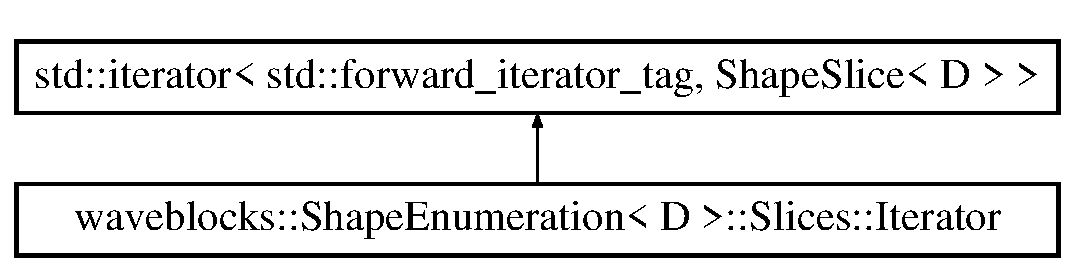
\includegraphics[height=2.000000cm]{structwaveblocks_1_1_shape_enumeration_1_1_slices_1_1_iterator}
\end{center}
\end{figure}
\subsection*{Public Member Functions}
\begin{DoxyCompactItemize}
\item 
\hypertarget{structwaveblocks_1_1_shape_enumeration_1_1_slices_1_1_iterator_adc6ee741b2b90c67cff8d8307ce71722}{}{\bfseries Iterator} (const \hyperlink{classwaveblocks_1_1_shape_enumeration}{Shape\+Enumeration} $\ast$ref, std\+::size\+\_\+t islice)\label{structwaveblocks_1_1_shape_enumeration_1_1_slices_1_1_iterator_adc6ee741b2b90c67cff8d8307ce71722}

\item 
\hypertarget{structwaveblocks_1_1_shape_enumeration_1_1_slices_1_1_iterator_a2733df5e6d2ae06824c5e9ddab922243}{}{\bfseries Iterator} (const \hyperlink{structwaveblocks_1_1_shape_enumeration_1_1_slices_1_1_iterator}{Iterator} \&other)\label{structwaveblocks_1_1_shape_enumeration_1_1_slices_1_1_iterator_a2733df5e6d2ae06824c5e9ddab922243}

\item 
\hypertarget{structwaveblocks_1_1_shape_enumeration_1_1_slices_1_1_iterator_aed34a557b48491f377ec837f5e51470c}{}\hyperlink{structwaveblocks_1_1_shape_enumeration_1_1_slices_1_1_iterator}{Iterator} \& {\bfseries operator=} (const \hyperlink{structwaveblocks_1_1_shape_enumeration_1_1_slices_1_1_iterator}{Iterator} \&other) const \label{structwaveblocks_1_1_shape_enumeration_1_1_slices_1_1_iterator_aed34a557b48491f377ec837f5e51470c}

\item 
\hypertarget{structwaveblocks_1_1_shape_enumeration_1_1_slices_1_1_iterator_a00e607e1b562f771f9bd6c637fcf120f}{}bool {\bfseries operator!=} (const \hyperlink{structwaveblocks_1_1_shape_enumeration_1_1_slices_1_1_iterator}{Iterator} \&other) const \label{structwaveblocks_1_1_shape_enumeration_1_1_slices_1_1_iterator_a00e607e1b562f771f9bd6c637fcf120f}

\item 
\hypertarget{structwaveblocks_1_1_shape_enumeration_1_1_slices_1_1_iterator_a09b8883d0dbc1063fb3486e06524b6d3}{}bool {\bfseries operator==} (const \hyperlink{structwaveblocks_1_1_shape_enumeration_1_1_slices_1_1_iterator}{Iterator} \&other) const \label{structwaveblocks_1_1_shape_enumeration_1_1_slices_1_1_iterator_a09b8883d0dbc1063fb3486e06524b6d3}

\item 
\hypertarget{structwaveblocks_1_1_shape_enumeration_1_1_slices_1_1_iterator_a30d9774204e3ef2b4303d197062fa714}{}const \hyperlink{classwaveblocks_1_1_shape_slice}{Shape\+Slice}$<$ D $>$ \& {\bfseries operator$\ast$} () const \label{structwaveblocks_1_1_shape_enumeration_1_1_slices_1_1_iterator_a30d9774204e3ef2b4303d197062fa714}

\item 
\hypertarget{structwaveblocks_1_1_shape_enumeration_1_1_slices_1_1_iterator_a675f74ba92865ead401dc34e508fc7d1}{}const \hyperlink{classwaveblocks_1_1_shape_slice}{Shape\+Slice}$<$ D $>$ $\ast$ {\bfseries operator-\/$>$} () const \label{structwaveblocks_1_1_shape_enumeration_1_1_slices_1_1_iterator_a675f74ba92865ead401dc34e508fc7d1}

\item 
\hypertarget{structwaveblocks_1_1_shape_enumeration_1_1_slices_1_1_iterator_a8b847aa2ee43347544cdd152fb8eea18}{}\hyperlink{structwaveblocks_1_1_shape_enumeration_1_1_slices_1_1_iterator}{Iterator} \& {\bfseries operator++} ()\label{structwaveblocks_1_1_shape_enumeration_1_1_slices_1_1_iterator_a8b847aa2ee43347544cdd152fb8eea18}

\item 
\hypertarget{structwaveblocks_1_1_shape_enumeration_1_1_slices_1_1_iterator_a21b62391685938d0ff3089888d202643}{}\hyperlink{structwaveblocks_1_1_shape_enumeration_1_1_slices_1_1_iterator}{Iterator} \& {\bfseries operator++} (int)\label{structwaveblocks_1_1_shape_enumeration_1_1_slices_1_1_iterator_a21b62391685938d0ff3089888d202643}

\end{DoxyCompactItemize}


The documentation for this struct was generated from the following file\+:\begin{DoxyCompactItemize}
\item 
/home/michaja/\+Documents/eth/libwaveblocks/waveblocks/shape\+\_\+enumeration\+\_\+base.\+hpp\end{DoxyCompactItemize}

\hypertarget{classwaveblocks_1_1_shape_slice_1_1_iterator}{}\section{waveblocks\+:\+:Shape\+Slice$<$ D $>$\+:\+:Iterator Class Reference}
\label{classwaveblocks_1_1_shape_slice_1_1_iterator}\index{waveblocks\+::\+Shape\+Slice$<$ D $>$\+::\+Iterator@{waveblocks\+::\+Shape\+Slice$<$ D $>$\+::\+Iterator}}


const\+\_\+iterator over a slice to support foreach statements  




{\ttfamily \#include $<$shape\+\_\+enumeration\+\_\+base.\+hpp$>$}

Inheritance diagram for waveblocks\+:\+:Shape\+Slice$<$ D $>$\+:\+:Iterator\+:\begin{figure}[H]
\begin{center}
\leavevmode
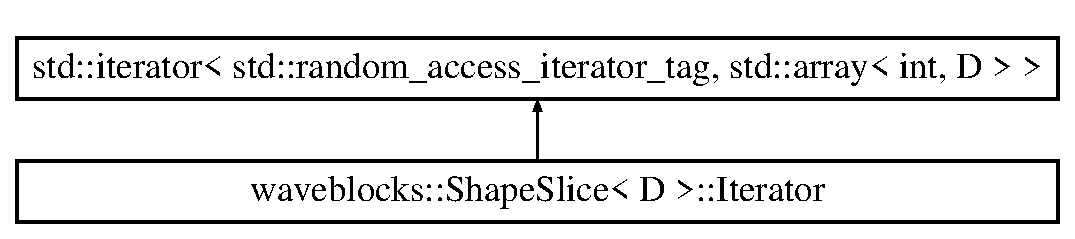
\includegraphics[height=2.000000cm]{classwaveblocks_1_1_shape_slice_1_1_iterator}
\end{center}
\end{figure}
\subsection*{Public Member Functions}
\begin{DoxyCompactItemize}
\item 
\hypertarget{classwaveblocks_1_1_shape_slice_1_1_iterator_a203d241011ee7157662e6cb850788557}{}{\bfseries Iterator} (const \hyperlink{classwaveblocks_1_1_shape_slice}{Shape\+Slice} $\ast$slice, std\+::size\+\_\+t ientry)\label{classwaveblocks_1_1_shape_slice_1_1_iterator_a203d241011ee7157662e6cb850788557}

\item 
\hypertarget{classwaveblocks_1_1_shape_slice_1_1_iterator_a4da1a023651f589fe6e137b4fef9893b}{}{\bfseries Iterator} (const \hyperlink{classwaveblocks_1_1_shape_slice_1_1_iterator}{Iterator} \&other)\label{classwaveblocks_1_1_shape_slice_1_1_iterator_a4da1a023651f589fe6e137b4fef9893b}

\item 
\hypertarget{classwaveblocks_1_1_shape_slice_1_1_iterator_adf1c460ac9b9172f5357cc4dbcdeec4d}{}\hyperlink{classwaveblocks_1_1_shape_slice_1_1_iterator}{Iterator} \& {\bfseries operator=} (const \hyperlink{classwaveblocks_1_1_shape_slice_1_1_iterator}{Iterator} \&other) const \label{classwaveblocks_1_1_shape_slice_1_1_iterator_adf1c460ac9b9172f5357cc4dbcdeec4d}

\item 
\hypertarget{classwaveblocks_1_1_shape_slice_1_1_iterator_a1cbe7161b640563f4a7bccf9fe867a2c}{}bool {\bfseries operator!=} (const \hyperlink{classwaveblocks_1_1_shape_slice_1_1_iterator}{Iterator} \&other) const \label{classwaveblocks_1_1_shape_slice_1_1_iterator_a1cbe7161b640563f4a7bccf9fe867a2c}

\item 
\hypertarget{classwaveblocks_1_1_shape_slice_1_1_iterator_a51b5b6b95be7d8a23db85d26c43630f5}{}bool {\bfseries operator==} (const \hyperlink{classwaveblocks_1_1_shape_slice_1_1_iterator}{Iterator} \&other) const \label{classwaveblocks_1_1_shape_slice_1_1_iterator_a51b5b6b95be7d8a23db85d26c43630f5}

\item 
\hypertarget{classwaveblocks_1_1_shape_slice_1_1_iterator_a9cea26703a7f1d3ff6c9af4b5c032b18}{}std\+::array$<$ int, D $>$ {\bfseries operator$\ast$} () const \label{classwaveblocks_1_1_shape_slice_1_1_iterator_a9cea26703a7f1d3ff6c9af4b5c032b18}

\item 
\hypertarget{classwaveblocks_1_1_shape_slice_1_1_iterator_ab3b184622be229294b4900bd36f87068}{}\hyperlink{classwaveblocks_1_1_shape_slice_1_1_iterator}{Iterator} \& {\bfseries operator++} ()\label{classwaveblocks_1_1_shape_slice_1_1_iterator_ab3b184622be229294b4900bd36f87068}

\item 
\hypertarget{classwaveblocks_1_1_shape_slice_1_1_iterator_a300c7933873797164ada89e3446d1022}{}\hyperlink{classwaveblocks_1_1_shape_slice_1_1_iterator}{Iterator} \& {\bfseries operator++} (int)\label{classwaveblocks_1_1_shape_slice_1_1_iterator_a300c7933873797164ada89e3446d1022}

\item 
\hypertarget{classwaveblocks_1_1_shape_slice_1_1_iterator_a1d559a2f035d05370f8a306e72f0e5cd}{}\hyperlink{classwaveblocks_1_1_shape_slice_1_1_iterator}{Iterator} \& {\bfseries operator-\/-\/} ()\label{classwaveblocks_1_1_shape_slice_1_1_iterator_a1d559a2f035d05370f8a306e72f0e5cd}

\item 
\hypertarget{classwaveblocks_1_1_shape_slice_1_1_iterator_a5cad6e00dd26e61cfe8c72d76c4d3df2}{}\hyperlink{classwaveblocks_1_1_shape_slice_1_1_iterator}{Iterator} \& {\bfseries operator-\/-\/} (int)\label{classwaveblocks_1_1_shape_slice_1_1_iterator_a5cad6e00dd26e61cfe8c72d76c4d3df2}

\item 
\hypertarget{classwaveblocks_1_1_shape_slice_1_1_iterator_a38a6465d2b031b80561fdce5111532dc}{}\hyperlink{classwaveblocks_1_1_shape_slice_1_1_iterator}{Iterator} \& {\bfseries operator+=} (std\+::ptrdiff\+\_\+t n)\label{classwaveblocks_1_1_shape_slice_1_1_iterator_a38a6465d2b031b80561fdce5111532dc}

\item 
\hypertarget{classwaveblocks_1_1_shape_slice_1_1_iterator_a28a22046ac1e96f570c183ac5639a1ca}{}\hyperlink{classwaveblocks_1_1_shape_slice_1_1_iterator}{Iterator} \& {\bfseries operator-\/=} (std\+::ptrdiff\+\_\+t n)\label{classwaveblocks_1_1_shape_slice_1_1_iterator_a28a22046ac1e96f570c183ac5639a1ca}

\item 
\hypertarget{classwaveblocks_1_1_shape_slice_1_1_iterator_a3824347da4f953a8f969147b23fabfd3}{}\hyperlink{classwaveblocks_1_1_shape_slice_1_1_iterator}{Iterator} {\bfseries operator+} (std\+::ptrdiff\+\_\+t n) const \label{classwaveblocks_1_1_shape_slice_1_1_iterator_a3824347da4f953a8f969147b23fabfd3}

\item 
\hypertarget{classwaveblocks_1_1_shape_slice_1_1_iterator_aa1f12d4ad57693ca1272736dc3dedb12}{}\hyperlink{classwaveblocks_1_1_shape_slice_1_1_iterator}{Iterator} {\bfseries operator-\/} (std\+::ptrdiff\+\_\+t n) const \label{classwaveblocks_1_1_shape_slice_1_1_iterator_aa1f12d4ad57693ca1272736dc3dedb12}

\item 
\hypertarget{classwaveblocks_1_1_shape_slice_1_1_iterator_a7d935bb6d747291867558e2343fb4704}{}std\+::array$<$ int, D $>$ {\bfseries operator\mbox{[}$\,$\mbox{]}} (std\+::ptrdiff\+\_\+t n) const \label{classwaveblocks_1_1_shape_slice_1_1_iterator_a7d935bb6d747291867558e2343fb4704}

\item 
\hypertarget{classwaveblocks_1_1_shape_slice_1_1_iterator_a4ddaac7ccc8802d464af1b9611d0ce40}{}bool {\bfseries operator$<$} (const \hyperlink{classwaveblocks_1_1_shape_slice_1_1_iterator}{Iterator} \&that) const \label{classwaveblocks_1_1_shape_slice_1_1_iterator_a4ddaac7ccc8802d464af1b9611d0ce40}

\item 
\hypertarget{classwaveblocks_1_1_shape_slice_1_1_iterator_ad03f71348fb7c1f67c531076d4d129a0}{}bool {\bfseries operator$>$} (const \hyperlink{classwaveblocks_1_1_shape_slice_1_1_iterator}{Iterator} \&that) const \label{classwaveblocks_1_1_shape_slice_1_1_iterator_ad03f71348fb7c1f67c531076d4d129a0}

\item 
\hypertarget{classwaveblocks_1_1_shape_slice_1_1_iterator_a0b789953983c612866b38c49cf7c8b27}{}bool {\bfseries operator$<$=} (const \hyperlink{classwaveblocks_1_1_shape_slice_1_1_iterator}{Iterator} \&that) const \label{classwaveblocks_1_1_shape_slice_1_1_iterator_a0b789953983c612866b38c49cf7c8b27}

\item 
\hypertarget{classwaveblocks_1_1_shape_slice_1_1_iterator_a7b7925a9710cc5cb39ae7f1efa62dcf5}{}bool {\bfseries operator$>$=} (const \hyperlink{classwaveblocks_1_1_shape_slice_1_1_iterator}{Iterator} \&that) const \label{classwaveblocks_1_1_shape_slice_1_1_iterator_a7b7925a9710cc5cb39ae7f1efa62dcf5}

\end{DoxyCompactItemize}


\subsection{Detailed Description}
\subsubsection*{template$<$dim\+\_\+t D$>$class waveblocks\+::\+Shape\+Slice$<$ D $>$\+::\+Iterator}

const\+\_\+iterator over a slice to support foreach statements 

The documentation for this class was generated from the following file\+:\begin{DoxyCompactItemize}
\item 
/home/michaja/\+Documents/eth/libwaveblocks/waveblocks/shape\+\_\+enumeration\+\_\+base.\+hpp\end{DoxyCompactItemize}

\hypertarget{classwaveblocks_1_1_kahan_sum}{}\section{waveblocks\+:\+:Kahan\+Sum$<$ T $>$ Class Template Reference}
\label{classwaveblocks_1_1_kahan_sum}\index{waveblocks\+::\+Kahan\+Sum$<$ T $>$@{waveblocks\+::\+Kahan\+Sum$<$ T $>$}}


The Kahan\textquotesingle{}s algorithm achieves O(1) error growth for summing N numbers.  




{\ttfamily \#include $<$kahan\+\_\+sum.\+hpp$>$}

\subsection*{Public Member Functions}
\begin{DoxyCompactItemize}
\item 
\hyperlink{classwaveblocks_1_1_kahan_sum_a14f2375af4f7a2d537a93a4e385a1da1}{Kahan\+Sum} ()=default
\begin{DoxyCompactList}\small\item\em compiler-\/generated default constructor \end{DoxyCompactList}\item 
\hyperlink{classwaveblocks_1_1_kahan_sum_ae81c0305e5c2f1188154e3265b33aed7}{Kahan\+Sum} (const T \&zero)
\begin{DoxyCompactList}\small\item\em A zero initializing constructor for types that cannot provide a default constructor. \end{DoxyCompactList}\item 
\hypertarget{classwaveblocks_1_1_kahan_sum_ab28e3b57ca3643290bcf245c478e1480}{}\hyperlink{classwaveblocks_1_1_kahan_sum_ab28e3b57ca3643290bcf245c478e1480}{Kahan\+Sum} (const \hyperlink{classwaveblocks_1_1_kahan_sum}{Kahan\+Sum}$<$ T $>$ \&that)=default\label{classwaveblocks_1_1_kahan_sum_ab28e3b57ca3643290bcf245c478e1480}

\begin{DoxyCompactList}\small\item\em compiler-\/generated copy constructor \end{DoxyCompactList}\item 
\hypertarget{classwaveblocks_1_1_kahan_sum_a45d992bd8ec6c417495c4df510c087aa}{}\hyperlink{classwaveblocks_1_1_kahan_sum}{Kahan\+Sum} \& \hyperlink{classwaveblocks_1_1_kahan_sum_a45d992bd8ec6c417495c4df510c087aa}{operator=} (const \hyperlink{classwaveblocks_1_1_kahan_sum}{Kahan\+Sum}$<$ T $>$ \&that)=default\label{classwaveblocks_1_1_kahan_sum_a45d992bd8ec6c417495c4df510c087aa}

\begin{DoxyCompactList}\small\item\em compiler-\/generated copy assignment operator \end{DoxyCompactList}\item 
\hyperlink{classwaveblocks_1_1_kahan_sum}{Kahan\+Sum} \& \hyperlink{classwaveblocks_1_1_kahan_sum_aee0ad6881394b6205e51bfb653f7bba0}{operator+=} (const T \&summand)
\begin{DoxyCompactList}\small\item\em adds a number \end{DoxyCompactList}\item 
const T \& \hyperlink{classwaveblocks_1_1_kahan_sum_ae737808fa3da9f853cfa9a2af06a2444}{operator()} () const 
\begin{DoxyCompactList}\small\item\em retrieves accumulated sum. \end{DoxyCompactList}\end{DoxyCompactItemize}


\subsection{Detailed Description}
\subsubsection*{template$<$class T$>$class waveblocks\+::\+Kahan\+Sum$<$ T $>$}

The Kahan\textquotesingle{}s algorithm achieves O(1) error growth for summing N numbers. 

This implementation works for every type that satisfies following requirements\+:
\begin{DoxyItemize}
\item copy constructor
\item copy assignment operator
\item binary plus operator that performs element-\/wise addition
\item binary minus operator that performs element-\/wise subtraction
\end{DoxyItemize}


\begin{DoxyTemplParams}{Template Parameters}
{\em T} & type of summands \\
\hline
\end{DoxyTemplParams}


\subsection{Constructor \& Destructor Documentation}
\hypertarget{classwaveblocks_1_1_kahan_sum_a14f2375af4f7a2d537a93a4e385a1da1}{}\index{waveblocks\+::\+Kahan\+Sum@{waveblocks\+::\+Kahan\+Sum}!Kahan\+Sum@{Kahan\+Sum}}
\index{Kahan\+Sum@{Kahan\+Sum}!waveblocks\+::\+Kahan\+Sum@{waveblocks\+::\+Kahan\+Sum}}
\subsubsection[{Kahan\+Sum}]{\setlength{\rightskip}{0pt plus 5cm}template$<$class T$>$ {\bf waveblocks\+::\+Kahan\+Sum}$<$ T $>$\+::{\bf Kahan\+Sum} (
\begin{DoxyParamCaption}
{}
\end{DoxyParamCaption}
)\hspace{0.3cm}{\ttfamily [default]}}\label{classwaveblocks_1_1_kahan_sum_a14f2375af4f7a2d537a93a4e385a1da1}


compiler-\/generated default constructor 

Be aware that this constructor fails on summand types that cannot provide a default constructor like dynamically sized arrays/matrices.

\begin{DoxySeeAlso}{See also}
\hyperlink{classwaveblocks_1_1_kahan_sum_ae81c0305e5c2f1188154e3265b33aed7}{Kahan\+Sum\+::\+Kahan\+Sum(const T\&)} 
\end{DoxySeeAlso}
\hypertarget{classwaveblocks_1_1_kahan_sum_ae81c0305e5c2f1188154e3265b33aed7}{}\index{waveblocks\+::\+Kahan\+Sum@{waveblocks\+::\+Kahan\+Sum}!Kahan\+Sum@{Kahan\+Sum}}
\index{Kahan\+Sum@{Kahan\+Sum}!waveblocks\+::\+Kahan\+Sum@{waveblocks\+::\+Kahan\+Sum}}
\subsubsection[{Kahan\+Sum}]{\setlength{\rightskip}{0pt plus 5cm}template$<$class T$>$ {\bf waveblocks\+::\+Kahan\+Sum}$<$ T $>$\+::{\bf Kahan\+Sum} (
\begin{DoxyParamCaption}
\item[{const T \&}]{zero}
\end{DoxyParamCaption}
)\hspace{0.3cm}{\ttfamily [inline]}}\label{classwaveblocks_1_1_kahan_sum_ae81c0305e5c2f1188154e3265b33aed7}


A zero initializing constructor for types that cannot provide a default constructor. 

A noteable example is a dynamically sized matrix.


\begin{DoxyParams}[1]{Parameters}
\mbox{\tt in}  & {\em zero} & initialized zero value as a template \\
\hline
\end{DoxyParams}


\subsection{Member Function Documentation}
\hypertarget{classwaveblocks_1_1_kahan_sum_ae737808fa3da9f853cfa9a2af06a2444}{}\index{waveblocks\+::\+Kahan\+Sum@{waveblocks\+::\+Kahan\+Sum}!operator()@{operator()}}
\index{operator()@{operator()}!waveblocks\+::\+Kahan\+Sum@{waveblocks\+::\+Kahan\+Sum}}
\subsubsection[{operator()}]{\setlength{\rightskip}{0pt plus 5cm}template$<$class T$>$ const T\& {\bf waveblocks\+::\+Kahan\+Sum}$<$ T $>$\+::operator() (
\begin{DoxyParamCaption}
{}
\end{DoxyParamCaption}
) const\hspace{0.3cm}{\ttfamily [inline]}}\label{classwaveblocks_1_1_kahan_sum_ae737808fa3da9f853cfa9a2af06a2444}


retrieves accumulated sum. 

\begin{DoxyReturn}{Returns}
accumulated sum 
\end{DoxyReturn}
\hypertarget{classwaveblocks_1_1_kahan_sum_aee0ad6881394b6205e51bfb653f7bba0}{}\index{waveblocks\+::\+Kahan\+Sum@{waveblocks\+::\+Kahan\+Sum}!operator+=@{operator+=}}
\index{operator+=@{operator+=}!waveblocks\+::\+Kahan\+Sum@{waveblocks\+::\+Kahan\+Sum}}
\subsubsection[{operator+=}]{\setlength{\rightskip}{0pt plus 5cm}template$<$class T$>$ {\bf Kahan\+Sum}\& {\bf waveblocks\+::\+Kahan\+Sum}$<$ T $>$\+::operator+= (
\begin{DoxyParamCaption}
\item[{const T \&}]{summand}
\end{DoxyParamCaption}
)\hspace{0.3cm}{\ttfamily [inline]}}\label{classwaveblocks_1_1_kahan_sum_aee0ad6881394b6205e51bfb653f7bba0}


adds a number 


\begin{DoxyParams}[1]{Parameters}
\mbox{\tt in}  & {\em summand} & summand \\
\hline
\end{DoxyParams}


The documentation for this class was generated from the following file\+:\begin{DoxyCompactItemize}
\item 
/home/michaja/\+Documents/eth/libwaveblocks/waveblocks/kahan\+\_\+sum.\+hpp\end{DoxyCompactItemize}

\hypertarget{structstd_1_1less_3_01waveblocks_1_1_tiny_multi_index_3_01_u_i_n_t_00_01_d_01_4_01_4}{}\section{std\+:\+:less$<$ waveblocks\+:\+:Tiny\+Multi\+Index$<$ U\+I\+N\+T, D $>$ $>$ Struct Template Reference}
\label{structstd_1_1less_3_01waveblocks_1_1_tiny_multi_index_3_01_u_i_n_t_00_01_d_01_4_01_4}\index{std\+::less$<$ waveblocks\+::\+Tiny\+Multi\+Index$<$ U\+I\+N\+T, D $>$ $>$@{std\+::less$<$ waveblocks\+::\+Tiny\+Multi\+Index$<$ U\+I\+N\+T, D $>$ $>$}}


{\ttfamily \#include $<$tiny\+\_\+multi\+\_\+index.\+hpp$>$}

\subsection*{Public Types}
\begin{DoxyCompactItemize}
\item 
\hypertarget{structstd_1_1less_3_01waveblocks_1_1_tiny_multi_index_3_01_u_i_n_t_00_01_d_01_4_01_4_aae355d29ecb3529615ea781af3e67997}{}typedef \hyperlink{classwaveblocks_1_1_tiny_multi_index}{Multi\+Index} {\bfseries first\+\_\+argument\+\_\+type}\label{structstd_1_1less_3_01waveblocks_1_1_tiny_multi_index_3_01_u_i_n_t_00_01_d_01_4_01_4_aae355d29ecb3529615ea781af3e67997}

\item 
\hypertarget{structstd_1_1less_3_01waveblocks_1_1_tiny_multi_index_3_01_u_i_n_t_00_01_d_01_4_01_4_a14f40a92cec3d63ff435e533953f7a20}{}typedef \hyperlink{classwaveblocks_1_1_tiny_multi_index}{Multi\+Index} {\bfseries second\+\_\+argument\+\_\+type}\label{structstd_1_1less_3_01waveblocks_1_1_tiny_multi_index_3_01_u_i_n_t_00_01_d_01_4_01_4_a14f40a92cec3d63ff435e533953f7a20}

\item 
\hypertarget{structstd_1_1less_3_01waveblocks_1_1_tiny_multi_index_3_01_u_i_n_t_00_01_d_01_4_01_4_ae6adf13e35fd3b3a498f7ecc7fd900d4}{}typedef bool {\bfseries result\+\_\+type}\label{structstd_1_1less_3_01waveblocks_1_1_tiny_multi_index_3_01_u_i_n_t_00_01_d_01_4_01_4_ae6adf13e35fd3b3a498f7ecc7fd900d4}

\end{DoxyCompactItemize}
\subsection*{Public Member Functions}
\begin{DoxyCompactItemize}
\item 
\hypertarget{structstd_1_1less_3_01waveblocks_1_1_tiny_multi_index_3_01_u_i_n_t_00_01_d_01_4_01_4_a1cd256d8f01a89874863e6aebc8133d0}{}bool {\bfseries operator()} (const \hyperlink{classwaveblocks_1_1_tiny_multi_index}{Multi\+Index} \&first, const \hyperlink{classwaveblocks_1_1_tiny_multi_index}{Multi\+Index} \&second) const \label{structstd_1_1less_3_01waveblocks_1_1_tiny_multi_index_3_01_u_i_n_t_00_01_d_01_4_01_4_a1cd256d8f01a89874863e6aebc8133d0}

\end{DoxyCompactItemize}


\subsection{Detailed Description}
\subsubsection*{template$<$class U\+I\+N\+T, waveblocks\+::dim\+\_\+t D$>$struct std\+::less$<$ waveblocks\+::\+Tiny\+Multi\+Index$<$ U\+I\+N\+T, D $>$ $>$}

provides less functor (compare) for S\+T\+L (notable std\+::map) specializes generic std\+::less$<$\+T$>$ 

The documentation for this struct was generated from the following file\+:\begin{DoxyCompactItemize}
\item 
/home/michaja/\+Documents/eth/libwaveblocks/waveblocks/tiny\+\_\+multi\+\_\+index.\+hpp\end{DoxyCompactItemize}

\hypertarget{classwaveblocks_1_1_lexical_index_generator}{}\section{waveblocks\+:\+:Lexical\+Index\+Generator$<$ D, Multi\+Index, S $>$ Class Template Reference}
\label{classwaveblocks_1_1_lexical_index_generator}\index{waveblocks\+::\+Lexical\+Index\+Generator$<$ D, Multi\+Index, S $>$@{waveblocks\+::\+Lexical\+Index\+Generator$<$ D, Multi\+Index, S $>$}}
\subsection*{Public Member Functions}
\begin{DoxyCompactItemize}
\item 
\hypertarget{classwaveblocks_1_1_lexical_index_generator_a1a0a38f8706ce6198ea68598fdcd1de3}{}{\bfseries Lexical\+Index\+Generator} (S shape)\label{classwaveblocks_1_1_lexical_index_generator_a1a0a38f8706ce6198ea68598fdcd1de3}

\item 
\hypertarget{classwaveblocks_1_1_lexical_index_generator_a1a48f523968fda75e151898fced283b6}{}{\bfseries Lexical\+Index\+Generator} (S shape, Multi\+Index index)\label{classwaveblocks_1_1_lexical_index_generator_a1a48f523968fda75e151898fced283b6}

\item 
\hypertarget{classwaveblocks_1_1_lexical_index_generator_ac3ba6069521e3ec394c2f4f8025ac6d9}{}{\bfseries Lexical\+Index\+Generator} (const \hyperlink{classwaveblocks_1_1_lexical_index_generator}{Lexical\+Index\+Generator} \&that)\label{classwaveblocks_1_1_lexical_index_generator_ac3ba6069521e3ec394c2f4f8025ac6d9}

\item 
\hypertarget{classwaveblocks_1_1_lexical_index_generator_a25490f7b4ee18d19b681739c29c41c9a}{}\hyperlink{classwaveblocks_1_1_lexical_index_generator}{Lexical\+Index\+Generator} \& {\bfseries operator=} (const \hyperlink{classwaveblocks_1_1_lexical_index_generator}{Lexical\+Index\+Generator} \&that)\label{classwaveblocks_1_1_lexical_index_generator_a25490f7b4ee18d19b681739c29c41c9a}

\item 
\hypertarget{classwaveblocks_1_1_lexical_index_generator_a6ad27c94d3cb50c15ca0bc6bce3a031f}{}Multi\+Index {\bfseries index} () const \label{classwaveblocks_1_1_lexical_index_generator_a6ad27c94d3cb50c15ca0bc6bce3a031f}

\item 
\hypertarget{classwaveblocks_1_1_lexical_index_generator_a0c305c5ce1b0964c1556a9ba1d307cc5}{}bool {\bfseries backward} ()\label{classwaveblocks_1_1_lexical_index_generator_a0c305c5ce1b0964c1556a9ba1d307cc5}

\item 
\hypertarget{classwaveblocks_1_1_lexical_index_generator_adbad07c3469682311430d9824bdd1f3a}{}bool {\bfseries forward} ()\label{classwaveblocks_1_1_lexical_index_generator_adbad07c3469682311430d9824bdd1f3a}

\end{DoxyCompactItemize}


The documentation for this class was generated from the following file\+:\begin{DoxyCompactItemize}
\item 
/home/michaja/\+Documents/eth/libwaveblocks/waveblocks/lexical\+\_\+shape\+\_\+enumerator.\+hpp\end{DoxyCompactItemize}

\hypertarget{classwaveblocks_1_1_limited_hyperbolic_cut_shape}{}\section{waveblocks\+:\+:Limited\+Hyperbolic\+Cut\+Shape$<$ D $>$ Class Template Reference}
\label{classwaveblocks_1_1_limited_hyperbolic_cut_shape}\index{waveblocks\+::\+Limited\+Hyperbolic\+Cut\+Shape$<$ D $>$@{waveblocks\+::\+Limited\+Hyperbolic\+Cut\+Shape$<$ D $>$}}


{\ttfamily \#include $<$shape\+\_\+hyperbolic.\+hpp$>$}

\subsection*{Public Member Functions}
\begin{DoxyCompactItemize}
\item 
\hyperlink{classwaveblocks_1_1_limited_hyperbolic_cut_shape_a7e465bada711731a921b158d3222fa83}{Limited\+Hyperbolic\+Cut\+Shape} (int S, const std\+::array$<$ int, D $>$ \&limits)
\begin{DoxyCompactList}\small\item\em General constructor to define sparsity parameter and limits. \end{DoxyCompactList}\item 
\hyperlink{classwaveblocks_1_1_limited_hyperbolic_cut_shape_aec560dd3f0320fcd47df5ccc8f361f94}{Limited\+Hyperbolic\+Cut\+Shape} (int S, int size)
\begin{DoxyCompactList}\small\item\em Specialized constructor to set all limits $ K_d $ to the same value $ K^\star $. \end{DoxyCompactList}\item 
\hyperlink{classwaveblocks_1_1_limited_hyperbolic_cut_shape_affbff3fcfc3714f82d2e85261237f5a6}{Limited\+Hyperbolic\+Cut\+Shape} (int S, std\+::initializer\+\_\+list$<$ int $>$ list)
\begin{DoxyCompactList}\small\item\em General constructor to define sparsity parameter and limits. \end{DoxyCompactList}\item 
int \hyperlink{classwaveblocks_1_1_limited_hyperbolic_cut_shape_a0be64cd821d747288934130e5a43d2f6}{bbox} (dim\+\_\+t axis) const 
\item 
{\footnotesize template$<$class Multi\+Index $>$ }\\int \hyperlink{classwaveblocks_1_1_limited_hyperbolic_cut_shape_a3ecd60f8af667f143ce4798674ccb7f9}{limit} (const Multi\+Index \&base\+\_\+node, dim\+\_\+t axis) const 
\item 
\hypertarget{classwaveblocks_1_1_limited_hyperbolic_cut_shape_af1162aedf0ae6d18607fe4a783cb251f}{}std\+::string {\bfseries description} () const \label{classwaveblocks_1_1_limited_hyperbolic_cut_shape_af1162aedf0ae6d18607fe4a783cb251f}

\end{DoxyCompactItemize}


\subsection{Detailed Description}
\subsubsection*{template$<$dim\+\_\+t D$>$class waveblocks\+::\+Limited\+Hyperbolic\+Cut\+Shape$<$ D $>$}

This class implements the hyperbolic cut basis shape which is a special type of sparse basis set. A basis shape is essentially all information and operations related to the set $ \mathfrak{K} $ of multi-\/indices $ \boldsymbol{k} $. The limited hyperbolic cut shape in $ D $ dimensions with {\itshape sparsity} $S$ and {\itshape limits} $ \boldsymbol{K} = (K_1,\ldots,K_D) $ is defined as the set

\[ \mathfrak{K}(D,S,\boldsymbol{K}) := \left\{(k_1,\dots,k_D) \mid 0 \leq k_d < K_d \; \forall d \in \{ 1,\ldots,D \} \land \displaystyle\prod_{d=1}^{D} (1+k_d) \leq S \right\} \]


\begin{DoxyTemplParams}{Template Parameters}
{\em D} & number of dimensions \\
\hline
\end{DoxyTemplParams}


\subsection{Constructor \& Destructor Documentation}
\hypertarget{classwaveblocks_1_1_limited_hyperbolic_cut_shape_a7e465bada711731a921b158d3222fa83}{}\index{waveblocks\+::\+Limited\+Hyperbolic\+Cut\+Shape@{waveblocks\+::\+Limited\+Hyperbolic\+Cut\+Shape}!Limited\+Hyperbolic\+Cut\+Shape@{Limited\+Hyperbolic\+Cut\+Shape}}
\index{Limited\+Hyperbolic\+Cut\+Shape@{Limited\+Hyperbolic\+Cut\+Shape}!waveblocks\+::\+Limited\+Hyperbolic\+Cut\+Shape@{waveblocks\+::\+Limited\+Hyperbolic\+Cut\+Shape}}
\subsubsection[{Limited\+Hyperbolic\+Cut\+Shape}]{\setlength{\rightskip}{0pt plus 5cm}template$<$dim\+\_\+t D$>$ {\bf waveblocks\+::\+Limited\+Hyperbolic\+Cut\+Shape}$<$ D $>$\+::{\bf Limited\+Hyperbolic\+Cut\+Shape} (
\begin{DoxyParamCaption}
\item[{int}]{S, }
\item[{const std\+::array$<$ int, D $>$ \&}]{limits}
\end{DoxyParamCaption}
)\hspace{0.3cm}{\ttfamily [inline]}}\label{classwaveblocks_1_1_limited_hyperbolic_cut_shape_a7e465bada711731a921b158d3222fa83}


General constructor to define sparsity parameter and limits. 


\begin{DoxyParams}{Parameters}
{\em S} & sparsity parameter $ S $ \\
\hline
{\em limits} & tuple of all limits $ \boldsymbol{K} $ \\
\hline
\end{DoxyParams}
\hypertarget{classwaveblocks_1_1_limited_hyperbolic_cut_shape_aec560dd3f0320fcd47df5ccc8f361f94}{}\index{waveblocks\+::\+Limited\+Hyperbolic\+Cut\+Shape@{waveblocks\+::\+Limited\+Hyperbolic\+Cut\+Shape}!Limited\+Hyperbolic\+Cut\+Shape@{Limited\+Hyperbolic\+Cut\+Shape}}
\index{Limited\+Hyperbolic\+Cut\+Shape@{Limited\+Hyperbolic\+Cut\+Shape}!waveblocks\+::\+Limited\+Hyperbolic\+Cut\+Shape@{waveblocks\+::\+Limited\+Hyperbolic\+Cut\+Shape}}
\subsubsection[{Limited\+Hyperbolic\+Cut\+Shape}]{\setlength{\rightskip}{0pt plus 5cm}template$<$dim\+\_\+t D$>$ {\bf waveblocks\+::\+Limited\+Hyperbolic\+Cut\+Shape}$<$ D $>$\+::{\bf Limited\+Hyperbolic\+Cut\+Shape} (
\begin{DoxyParamCaption}
\item[{int}]{S, }
\item[{int}]{size}
\end{DoxyParamCaption}
)\hspace{0.3cm}{\ttfamily [inline]}}\label{classwaveblocks_1_1_limited_hyperbolic_cut_shape_aec560dd3f0320fcd47df5ccc8f361f94}


Specialized constructor to set all limits $ K_d $ to the same value $ K^\star $. 


\begin{DoxyParams}{Parameters}
{\em S} & sparsity parameter $ S $ \\
\hline
{\em size} & $ K^\star $ \\
\hline
\end{DoxyParams}
\hypertarget{classwaveblocks_1_1_limited_hyperbolic_cut_shape_affbff3fcfc3714f82d2e85261237f5a6}{}\index{waveblocks\+::\+Limited\+Hyperbolic\+Cut\+Shape@{waveblocks\+::\+Limited\+Hyperbolic\+Cut\+Shape}!Limited\+Hyperbolic\+Cut\+Shape@{Limited\+Hyperbolic\+Cut\+Shape}}
\index{Limited\+Hyperbolic\+Cut\+Shape@{Limited\+Hyperbolic\+Cut\+Shape}!waveblocks\+::\+Limited\+Hyperbolic\+Cut\+Shape@{waveblocks\+::\+Limited\+Hyperbolic\+Cut\+Shape}}
\subsubsection[{Limited\+Hyperbolic\+Cut\+Shape}]{\setlength{\rightskip}{0pt plus 5cm}template$<$dim\+\_\+t D$>$ {\bf waveblocks\+::\+Limited\+Hyperbolic\+Cut\+Shape}$<$ D $>$\+::{\bf Limited\+Hyperbolic\+Cut\+Shape} (
\begin{DoxyParamCaption}
\item[{int}]{S, }
\item[{std\+::initializer\+\_\+list$<$ int $>$}]{list}
\end{DoxyParamCaption}
)\hspace{0.3cm}{\ttfamily [inline]}}\label{classwaveblocks_1_1_limited_hyperbolic_cut_shape_affbff3fcfc3714f82d2e85261237f5a6}


General constructor to define sparsity parameter and limits. 


\begin{DoxyParams}{Parameters}
{\em S} & sparsity parameter $ S $ \\
\hline
{\em list} & list of all limits $ \boldsymbol{K} $ \\
\hline
\end{DoxyParams}


\subsection{Member Function Documentation}
\hypertarget{classwaveblocks_1_1_limited_hyperbolic_cut_shape_a0be64cd821d747288934130e5a43d2f6}{}\index{waveblocks\+::\+Limited\+Hyperbolic\+Cut\+Shape@{waveblocks\+::\+Limited\+Hyperbolic\+Cut\+Shape}!bbox@{bbox}}
\index{bbox@{bbox}!waveblocks\+::\+Limited\+Hyperbolic\+Cut\+Shape@{waveblocks\+::\+Limited\+Hyperbolic\+Cut\+Shape}}
\subsubsection[{bbox}]{\setlength{\rightskip}{0pt plus 5cm}template$<$dim\+\_\+t D$>$ int {\bf waveblocks\+::\+Limited\+Hyperbolic\+Cut\+Shape}$<$ D $>$\+::bbox (
\begin{DoxyParamCaption}
\item[{dim\+\_\+t}]{axis}
\end{DoxyParamCaption}
) const\hspace{0.3cm}{\ttfamily [inline]}}\label{classwaveblocks_1_1_limited_hyperbolic_cut_shape_a0be64cd821d747288934130e5a43d2f6}
\begin{DoxySeeAlso}{See also}
\hyperlink{classwaveblocks_1_1_hyper_cubic_shape_a5e23e83ffa06b5486b5c7fd033dadbfa}{Hyper\+Cubic\+Shape\+::bbox} 
\end{DoxySeeAlso}
\hypertarget{classwaveblocks_1_1_limited_hyperbolic_cut_shape_a3ecd60f8af667f143ce4798674ccb7f9}{}\index{waveblocks\+::\+Limited\+Hyperbolic\+Cut\+Shape@{waveblocks\+::\+Limited\+Hyperbolic\+Cut\+Shape}!limit@{limit}}
\index{limit@{limit}!waveblocks\+::\+Limited\+Hyperbolic\+Cut\+Shape@{waveblocks\+::\+Limited\+Hyperbolic\+Cut\+Shape}}
\subsubsection[{limit}]{\setlength{\rightskip}{0pt plus 5cm}template$<$dim\+\_\+t D$>$ template$<$class Multi\+Index $>$ int {\bf waveblocks\+::\+Limited\+Hyperbolic\+Cut\+Shape}$<$ D $>$\+::limit (
\begin{DoxyParamCaption}
\item[{const Multi\+Index \&}]{base\+\_\+node, }
\item[{dim\+\_\+t}]{axis}
\end{DoxyParamCaption}
) const\hspace{0.3cm}{\ttfamily [inline]}}\label{classwaveblocks_1_1_limited_hyperbolic_cut_shape_a3ecd60f8af667f143ce4798674ccb7f9}
\begin{DoxySeeAlso}{See also}
\hyperlink{classwaveblocks_1_1_hyper_cubic_shape_a9b11ef910f9f914149a35e2f6ccc52e3}{Hyper\+Cubic\+Shape\+::limit} 
\end{DoxySeeAlso}


The documentation for this class was generated from the following file\+:\begin{DoxyCompactItemize}
\item 
/home/michaja/\+Documents/eth/libwaveblocks/waveblocks/shape\+\_\+hyperbolic.\+hpp\end{DoxyCompactItemize}

\hypertarget{classwaveblocks_1_1_shape_enumeration}{}\section{waveblocks\+:\+:Shape\+Enumeration$<$ D $>$ Class Template Reference}
\label{classwaveblocks_1_1_shape_enumeration}\index{waveblocks\+::\+Shape\+Enumeration$<$ D $>$@{waveblocks\+::\+Shape\+Enumeration$<$ D $>$}}


Assigns all multi-\/indices of a shape an ordinal.  




{\ttfamily \#include $<$shape\+\_\+enumeration\+\_\+base.\+hpp$>$}

Inheritance diagram for waveblocks\+:\+:Shape\+Enumeration$<$ D $>$\+:\begin{figure}[H]
\begin{center}
\leavevmode
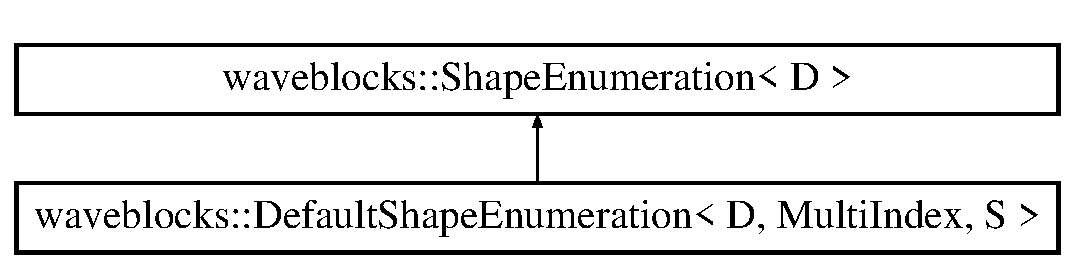
\includegraphics[height=2.000000cm]{classwaveblocks_1_1_shape_enumeration}
\end{center}
\end{figure}
\subsection*{Classes}
\begin{DoxyCompactItemize}
\item 
struct \hyperlink{structwaveblocks_1_1_shape_enumeration_1_1_slices}{Slices}
\begin{DoxyCompactList}\small\item\em range that contains all slices \end{DoxyCompactList}\end{DoxyCompactItemize}
\subsection*{Public Member Functions}
\begin{DoxyCompactItemize}
\item 
virtual std\+::size\+\_\+t \hyperlink{classwaveblocks_1_1_shape_enumeration_a6400c5e4f36b8077b253a18e91d07fb4}{n\+\_\+slices} () const =0
\item 
virtual const \hyperlink{classwaveblocks_1_1_shape_slice}{Shape\+Slice}$<$ D $>$ \& \hyperlink{classwaveblocks_1_1_shape_enumeration_abb6ab9207b189e4e7b5e67345c4f2ea9}{slice} (std\+::size\+\_\+t islice) const =0
\item 
virtual bool \hyperlink{classwaveblocks_1_1_shape_enumeration_af34f5d866923c3f4efc16dec49b4748d}{contains} (const std\+::array$<$ int, D $>$ \&index) const =0
\item 
virtual int \hyperlink{classwaveblocks_1_1_shape_enumeration_a35eb99f86fca58c2983cf8b00432e8c2}{bbox} (dim\+\_\+t axis) const =0
\begin{DoxyCompactList}\small\item\em retrieves the index of the outmost node in a given axis \end{DoxyCompactList}\item 
virtual std\+::size\+\_\+t \hyperlink{classwaveblocks_1_1_shape_enumeration_aa40d5659e3c109d8c77144208a9e1c2c}{size} () const 
\begin{DoxyCompactList}\small\item\em returns number of nodes that are part of the shape \end{DoxyCompactList}\item 
\hypertarget{classwaveblocks_1_1_shape_enumeration_a9b0fb82080a673dc1930d01844172cc0}{}\hyperlink{structwaveblocks_1_1_shape_enumeration_1_1_slices}{Slices} {\bfseries slices} () const \label{classwaveblocks_1_1_shape_enumeration_a9b0fb82080a673dc1930d01844172cc0}

\end{DoxyCompactItemize}


\subsection{Detailed Description}
\subsubsection*{template$<$dim\+\_\+t D$>$class waveblocks\+::\+Shape\+Enumeration$<$ D $>$}

Assigns all multi-\/indices of a shape an ordinal. 

Since many algorithms operating on wavepackets use recursive formulas, shape enumerations are divided into a set of {\itshape slices} to simplify data structures.

The $ s $-\/th slice contains all multi-\/indices $ \boldsymbol{k} \in \mathfrak{K} $ that satisfy $ \displaystyle\sum_{d=1}^{D} k_d = s $.

To determine, to which slice a multi-\/index belongs, do\+: 
\begin{DoxyCode}
\textcolor{preprocessor}{#include <algorithms>}
\textcolor{keywordtype}{int} islice = std::accumulate(index.begin(), index.end(), int(0));
\end{DoxyCode}
 

\subsection{Member Function Documentation}
\hypertarget{classwaveblocks_1_1_shape_enumeration_a35eb99f86fca58c2983cf8b00432e8c2}{}\index{waveblocks\+::\+Shape\+Enumeration@{waveblocks\+::\+Shape\+Enumeration}!bbox@{bbox}}
\index{bbox@{bbox}!waveblocks\+::\+Shape\+Enumeration@{waveblocks\+::\+Shape\+Enumeration}}
\subsubsection[{bbox}]{\setlength{\rightskip}{0pt plus 5cm}template$<$dim\+\_\+t D$>$ virtual int {\bf waveblocks\+::\+Shape\+Enumeration}$<$ D $>$\+::bbox (
\begin{DoxyParamCaption}
\item[{dim\+\_\+t}]{axis}
\end{DoxyParamCaption}
) const\hspace{0.3cm}{\ttfamily [pure virtual]}}\label{classwaveblocks_1_1_shape_enumeration_a35eb99f86fca58c2983cf8b00432e8c2}


retrieves the index of the outmost node in a given axis 

\begin{DoxyReturn}{Returns}

\end{DoxyReturn}


Implemented in \hyperlink{classwaveblocks_1_1_default_shape_enumeration_a6b6991c193523c2b66870c65c837b9e6}{waveblocks\+::\+Default\+Shape\+Enumeration$<$ D, Multi\+Index, S $>$}.

\hypertarget{classwaveblocks_1_1_shape_enumeration_af34f5d866923c3f4efc16dec49b4748d}{}\index{waveblocks\+::\+Shape\+Enumeration@{waveblocks\+::\+Shape\+Enumeration}!contains@{contains}}
\index{contains@{contains}!waveblocks\+::\+Shape\+Enumeration@{waveblocks\+::\+Shape\+Enumeration}}
\subsubsection[{contains}]{\setlength{\rightskip}{0pt plus 5cm}template$<$dim\+\_\+t D$>$ virtual bool {\bf waveblocks\+::\+Shape\+Enumeration}$<$ D $>$\+::contains (
\begin{DoxyParamCaption}
\item[{const std\+::array$<$ int, D $>$ \&}]{index}
\end{DoxyParamCaption}
) const\hspace{0.3cm}{\ttfamily [pure virtual]}}\label{classwaveblocks_1_1_shape_enumeration_af34f5d866923c3f4efc16dec49b4748d}
\begin{DoxyReturn}{Returns}
forwards 
\end{DoxyReturn}


Implemented in \hyperlink{classwaveblocks_1_1_default_shape_enumeration_a766b764e141186034ed942b25248f31a}{waveblocks\+::\+Default\+Shape\+Enumeration$<$ D, Multi\+Index, S $>$}.

\hypertarget{classwaveblocks_1_1_shape_enumeration_a6400c5e4f36b8077b253a18e91d07fb4}{}\index{waveblocks\+::\+Shape\+Enumeration@{waveblocks\+::\+Shape\+Enumeration}!n\+\_\+slices@{n\+\_\+slices}}
\index{n\+\_\+slices@{n\+\_\+slices}!waveblocks\+::\+Shape\+Enumeration@{waveblocks\+::\+Shape\+Enumeration}}
\subsubsection[{n\+\_\+slices}]{\setlength{\rightskip}{0pt plus 5cm}template$<$dim\+\_\+t D$>$ virtual std\+::size\+\_\+t {\bf waveblocks\+::\+Shape\+Enumeration}$<$ D $>$\+::n\+\_\+slices (
\begin{DoxyParamCaption}
{}
\end{DoxyParamCaption}
) const\hspace{0.3cm}{\ttfamily [pure virtual]}}\label{classwaveblocks_1_1_shape_enumeration_a6400c5e4f36b8077b253a18e91d07fb4}
\begin{DoxyReturn}{Returns}
number of (ideally non-\/empty) slices 
\end{DoxyReturn}


Implemented in \hyperlink{classwaveblocks_1_1_default_shape_enumeration_aab6571cd94ba28768c569626af5a66a3}{waveblocks\+::\+Default\+Shape\+Enumeration$<$ D, Multi\+Index, S $>$}.

\hypertarget{classwaveblocks_1_1_shape_enumeration_aa40d5659e3c109d8c77144208a9e1c2c}{}\index{waveblocks\+::\+Shape\+Enumeration@{waveblocks\+::\+Shape\+Enumeration}!size@{size}}
\index{size@{size}!waveblocks\+::\+Shape\+Enumeration@{waveblocks\+::\+Shape\+Enumeration}}
\subsubsection[{size}]{\setlength{\rightskip}{0pt plus 5cm}template$<$dim\+\_\+t D$>$ virtual std\+::size\+\_\+t {\bf waveblocks\+::\+Shape\+Enumeration}$<$ D $>$\+::size (
\begin{DoxyParamCaption}
{}
\end{DoxyParamCaption}
) const\hspace{0.3cm}{\ttfamily [inline]}, {\ttfamily [virtual]}}\label{classwaveblocks_1_1_shape_enumeration_aa40d5659e3c109d8c77144208a9e1c2c}


returns number of nodes that are part of the shape 

\begin{DoxyReturn}{Returns}
number of nodes 
\end{DoxyReturn}


Reimplemented in \hyperlink{classwaveblocks_1_1_default_shape_enumeration_a5fc46846d7763190f1911b542bfec103}{waveblocks\+::\+Default\+Shape\+Enumeration$<$ D, Multi\+Index, S $>$}.

\hypertarget{classwaveblocks_1_1_shape_enumeration_abb6ab9207b189e4e7b5e67345c4f2ea9}{}\index{waveblocks\+::\+Shape\+Enumeration@{waveblocks\+::\+Shape\+Enumeration}!slice@{slice}}
\index{slice@{slice}!waveblocks\+::\+Shape\+Enumeration@{waveblocks\+::\+Shape\+Enumeration}}
\subsubsection[{slice}]{\setlength{\rightskip}{0pt plus 5cm}template$<$dim\+\_\+t D$>$ virtual const {\bf Shape\+Slice}$<$D$>$\& {\bf waveblocks\+::\+Shape\+Enumeration}$<$ D $>$\+::slice (
\begin{DoxyParamCaption}
\item[{std\+::size\+\_\+t}]{islice}
\end{DoxyParamCaption}
) const\hspace{0.3cm}{\ttfamily [pure virtual]}}\label{classwaveblocks_1_1_shape_enumeration_abb6ab9207b189e4e7b5e67345c4f2ea9}

\begin{DoxyParams}[1]{Parameters}
\mbox{\tt in}  & {\em islice} & index of requested slice \\
\hline
\end{DoxyParams}
\begin{DoxyReturn}{Returns}
requested slice or empty slice if (islice $>$= \#slices) 
\end{DoxyReturn}


Implemented in \hyperlink{classwaveblocks_1_1_default_shape_enumeration_a323986feed57994f2049627e67cda2cc}{waveblocks\+::\+Default\+Shape\+Enumeration$<$ D, Multi\+Index, S $>$}.



The documentation for this class was generated from the following file\+:\begin{DoxyCompactItemize}
\item 
/home/michaja/\+Documents/eth/libwaveblocks/waveblocks/shape\+\_\+enumeration\+\_\+base.\+hpp\end{DoxyCompactItemize}

\hypertarget{classwaveblocks_1_1_shape_extension_enumeration}{}\section{waveblocks\+:\+:Shape\+Extension\+Enumeration$<$ D, S $>$ Class Template Reference}
\label{classwaveblocks_1_1_shape_extension_enumeration}\index{waveblocks\+::\+Shape\+Extension\+Enumeration$<$ D, S $>$@{waveblocks\+::\+Shape\+Extension\+Enumeration$<$ D, S $>$}}


{\ttfamily \#include $<$extension\+\_\+enumeration.\+hpp$>$}

\subsection*{Public Types}
\begin{DoxyCompactItemize}
\item 
\hypertarget{classwaveblocks_1_1_shape_extension_enumeration_af616a65a7c2bad0c405b658d178f7691}{}typedef std\+::vector$<$ Multi\+Index$<$ D $>$ $>$\+::const\+\_\+iterator {\bfseries Iterator}\label{classwaveblocks_1_1_shape_extension_enumeration_af616a65a7c2bad0c405b658d178f7691}

\end{DoxyCompactItemize}
\subsection*{Public Member Functions}
\begin{DoxyCompactItemize}
\item 
\hypertarget{classwaveblocks_1_1_shape_extension_enumeration_a4162a6b0024f247c0d26cfa2f84ef48c}{}{\bfseries Shape\+Extension\+Enumeration} (S shape)\label{classwaveblocks_1_1_shape_extension_enumeration_a4162a6b0024f247c0d26cfa2f84ef48c}

\item 
\hypertarget{classwaveblocks_1_1_shape_extension_enumeration_a063ff056516d79f8dba15eff2c96f740}{}{\bfseries Shape\+Extension\+Enumeration} (const \hyperlink{classwaveblocks_1_1_shape_extension_enumeration}{Shape\+Extension\+Enumeration} \&that)\label{classwaveblocks_1_1_shape_extension_enumeration_a063ff056516d79f8dba15eff2c96f740}

\item 
\hypertarget{classwaveblocks_1_1_shape_extension_enumeration_a1e7aa102629b723b7cf82024f80a24e0}{}\hyperlink{classwaveblocks_1_1_shape_extension_enumeration}{Shape\+Extension\+Enumeration} \& {\bfseries operator=} (const \hyperlink{classwaveblocks_1_1_shape_extension_enumeration}{Shape\+Extension\+Enumeration} \&that)\label{classwaveblocks_1_1_shape_extension_enumeration_a1e7aa102629b723b7cf82024f80a24e0}

\item 
\hypertarget{classwaveblocks_1_1_shape_extension_enumeration_af7feb054bebc01467ab94e05d776faf4}{}std\+::size\+\_\+t {\bfseries size} () const \label{classwaveblocks_1_1_shape_extension_enumeration_af7feb054bebc01467ab94e05d776faf4}

\item 
\hypertarget{classwaveblocks_1_1_shape_extension_enumeration_a436a73d6cf125e6b04bdcc04cea7b39c}{}std\+::size\+\_\+t {\bfseries find} (Multi\+Index$<$ D $>$ index) const \label{classwaveblocks_1_1_shape_extension_enumeration_a436a73d6cf125e6b04bdcc04cea7b39c}

\item 
\hypertarget{classwaveblocks_1_1_shape_extension_enumeration_abf04924f58894849ee311837d47c028c}{}Multi\+Index$<$ D $>$ {\bfseries operator\mbox{[}$\,$\mbox{]}} (std\+::size\+\_\+t ordinal) const \label{classwaveblocks_1_1_shape_extension_enumeration_abf04924f58894849ee311837d47c028c}

\item 
\hypertarget{classwaveblocks_1_1_shape_extension_enumeration_ac1b44cb4e86f97c5e63af11a5f761493}{}Iterator {\bfseries begin} () const \label{classwaveblocks_1_1_shape_extension_enumeration_ac1b44cb4e86f97c5e63af11a5f761493}

\item 
\hypertarget{classwaveblocks_1_1_shape_extension_enumeration_ab7b524f76fcb40f6208bd676ad1724d8}{}Iterator {\bfseries end} () const \label{classwaveblocks_1_1_shape_extension_enumeration_ab7b524f76fcb40f6208bd676ad1724d8}

\end{DoxyCompactItemize}


\subsection{Detailed Description}
\subsubsection*{template$<$dim\+\_\+t D, class S$>$class waveblocks\+::\+Shape\+Extension\+Enumeration$<$ D, S $>$}

Extended shapes are needed for the gradient computation of the wavepacket.

This class is not used anymore. The original idea was that the enumeration of the extended shape consists of two parts\+: The first part is equal to the enumeration of the original shape. This class forms the second part. It stores the additional nodes that are part of the shape extension \textquotesingle{}shell\textquotesingle{}. This saves some memory as the first part is identical to the enumeration of the corresponding basic shape. Since the gradient computation involves the evaluation of a wavepacket, this two-\/part idea implicates that two implementations of the evaluation are needed. One implementation for a wavepacket using a basic shape and one for using an extended shape. This two-\/part idea has been abandoned for the sake of simplicity.

This class has been fully tested and works. 

The documentation for this class was generated from the following file\+:\begin{DoxyCompactItemize}
\item 
/home/michaja/\+Documents/eth/libwaveblocks/waveblocks/extension\+\_\+enumeration.\+hpp\end{DoxyCompactItemize}

\hypertarget{classwaveblocks_1_1_shape_slice}{}\section{waveblocks\+:\+:Shape\+Slice$<$ D $>$ Class Template Reference}
\label{classwaveblocks_1_1_shape_slice}\index{waveblocks\+::\+Shape\+Slice$<$ D $>$@{waveblocks\+::\+Shape\+Slice$<$ D $>$}}
Inheritance diagram for waveblocks\+:\+:Shape\+Slice$<$ D $>$\+:\begin{figure}[H]
\begin{center}
\leavevmode
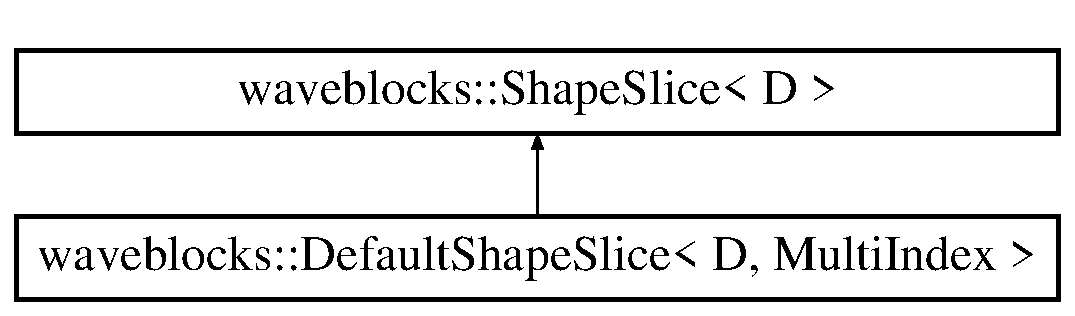
\includegraphics[height=2.000000cm]{classwaveblocks_1_1_shape_slice}
\end{center}
\end{figure}
\subsection*{Classes}
\begin{DoxyCompactItemize}
\item 
class \hyperlink{classwaveblocks_1_1_shape_slice_1_1_iterator}{Iterator}
\begin{DoxyCompactList}\small\item\em const\+\_\+iterator over a slice to support foreach statements \end{DoxyCompactList}\end{DoxyCompactItemize}
\subsection*{Public Member Functions}
\begin{DoxyCompactItemize}
\item 
virtual std\+::size\+\_\+t \hyperlink{classwaveblocks_1_1_shape_slice_a1304d3ca2c080b8258ddff233c2b1809}{offset} () const =0
\item 
virtual std\+::size\+\_\+t \hyperlink{classwaveblocks_1_1_shape_slice_aba345671b0dd4058d4b5de285d904689}{slice\+\_\+index} () const =0
\item 
virtual std\+::size\+\_\+t \hyperlink{classwaveblocks_1_1_shape_slice_a08b3fd43798dea6e4487e4b41d926f30}{size} () const =0
\item 
virtual std\+::array$<$ int, D $>$ \hyperlink{classwaveblocks_1_1_shape_slice_a1e7363a71777b680cafe370ea4be2fb1}{operator\mbox{[}$\,$\mbox{]}} (std\+::size\+\_\+t ordinal) const =0
\begin{DoxyCompactList}\small\item\em Returns the multi-\/index of the node at position {\itshape ordinal}. \end{DoxyCompactList}\item 
virtual std\+::size\+\_\+t \hyperlink{classwaveblocks_1_1_shape_slice_ab38e2bf39cd8d9a2c9a1028622b077b1}{find} (const std\+::array$<$ int, D $>$ \&index) const =0
\begin{DoxyCompactList}\small\item\em Returns the position of the node with multi-\/index {\ttfamily index}. \end{DoxyCompactList}\item 
virtual std\+::array$<$ std\+::size\+\_\+t, D $>$ \hyperlink{classwaveblocks_1_1_shape_slice_a724b4713602473f6a0b712cf32592ead}{find\+\_\+backward\+\_\+neighbours} (const std\+::array$<$ int, D $>$ \&index) const =0
\begin{DoxyCompactList}\small\item\em Retrieves ordinals of all backward neighbours of a given node very efficiently. \end{DoxyCompactList}\item 
\hypertarget{classwaveblocks_1_1_shape_slice_a843c26f6500f8497a641ef9815c8603e}{}\hyperlink{classwaveblocks_1_1_shape_slice_1_1_iterator}{Iterator} {\bfseries begin} () const \label{classwaveblocks_1_1_shape_slice_a843c26f6500f8497a641ef9815c8603e}

\item 
\hypertarget{classwaveblocks_1_1_shape_slice_a9c23b0136051e2e229be8035cc87ffa9}{}\hyperlink{classwaveblocks_1_1_shape_slice_1_1_iterator}{Iterator} {\bfseries end} () const \label{classwaveblocks_1_1_shape_slice_a9c23b0136051e2e229be8035cc87ffa9}

\end{DoxyCompactItemize}


\subsection{Member Function Documentation}
\hypertarget{classwaveblocks_1_1_shape_slice_ab38e2bf39cd8d9a2c9a1028622b077b1}{}\index{waveblocks\+::\+Shape\+Slice@{waveblocks\+::\+Shape\+Slice}!find@{find}}
\index{find@{find}!waveblocks\+::\+Shape\+Slice@{waveblocks\+::\+Shape\+Slice}}
\subsubsection[{find}]{\setlength{\rightskip}{0pt plus 5cm}template$<$dim\+\_\+t D$>$ virtual std\+::size\+\_\+t {\bf waveblocks\+::\+Shape\+Slice}$<$ D $>$\+::find (
\begin{DoxyParamCaption}
\item[{const std\+::array$<$ int, D $>$ \&}]{index}
\end{DoxyParamCaption}
) const\hspace{0.3cm}{\ttfamily [pure virtual]}}\label{classwaveblocks_1_1_shape_slice_ab38e2bf39cd8d9a2c9a1028622b077b1}


Returns the position of the node with multi-\/index {\ttfamily index}. 

Notice that the first node in the slice has position 0 (not 1 or \hyperlink{classwaveblocks_1_1_shape_slice_a1304d3ca2c080b8258ddff233c2b1809}{offset()}).

Portable programs should never call this function with an node that is not part of this slice since this causes {\itshape undefined} {\itshape behaviour}.

Use Shape\+Enumeration$<$\+D$>$\+::contains(index) to check whether this slice contains the given node.

{\bfseries complexity\+: }logarithmic in the number of slice-\/nodes


\begin{DoxyParams}[1]{Parameters}
\mbox{\tt in}  & {\em index} & multi-\/index of a node in this slice \\
\hline
\end{DoxyParams}
\begin{DoxyReturn}{Returns}
position of the specified node 
\end{DoxyReturn}


Implemented in \hyperlink{classwaveblocks_1_1_default_shape_slice_ae44dd6209de700b5a370f3815979b883}{waveblocks\+::\+Default\+Shape\+Slice$<$ D, Multi\+Index $>$}.

\hypertarget{classwaveblocks_1_1_shape_slice_a724b4713602473f6a0b712cf32592ead}{}\index{waveblocks\+::\+Shape\+Slice@{waveblocks\+::\+Shape\+Slice}!find\+\_\+backward\+\_\+neighbours@{find\+\_\+backward\+\_\+neighbours}}
\index{find\+\_\+backward\+\_\+neighbours@{find\+\_\+backward\+\_\+neighbours}!waveblocks\+::\+Shape\+Slice@{waveblocks\+::\+Shape\+Slice}}
\subsubsection[{find\+\_\+backward\+\_\+neighbours}]{\setlength{\rightskip}{0pt plus 5cm}template$<$dim\+\_\+t D$>$ virtual std\+::array$<$std\+::size\+\_\+t,D$>$ {\bf waveblocks\+::\+Shape\+Slice}$<$ D $>$\+::find\+\_\+backward\+\_\+neighbours (
\begin{DoxyParamCaption}
\item[{const std\+::array$<$ int, D $>$ \&}]{index}
\end{DoxyParamCaption}
) const\hspace{0.3cm}{\ttfamily [pure virtual]}}\label{classwaveblocks_1_1_shape_slice_a724b4713602473f6a0b712cf32592ead}


Retrieves ordinals of all backward neighbours of a given node very efficiently. 

Notice that this method assumes that the given node {\bfseries is part of the shape}. Therefore this method does not need to perform any contains()-\/checks since it knows that all backward neighbours exist, except when the given node contains some zero entries. In the latter case, this method returns an undefined ordinal.

If the given node is not part of the shape, then the behaviour is undefined.


\begin{DoxyParams}[1]{Parameters}
\mbox{\tt in}  & {\em index} & node that {\bfseries is part of the shape} \\
\hline
\end{DoxyParams}
\begin{DoxyReturn}{Returns}
For each backward neighbour its ordinal. An ordinal is undefined if its node does not exist. 
\end{DoxyReturn}


Implemented in \hyperlink{classwaveblocks_1_1_default_shape_slice_a798802b140b441811e9d5ac74b16fb53}{waveblocks\+::\+Default\+Shape\+Slice$<$ D, Multi\+Index $>$}.

\hypertarget{classwaveblocks_1_1_shape_slice_a1304d3ca2c080b8258ddff233c2b1809}{}\index{waveblocks\+::\+Shape\+Slice@{waveblocks\+::\+Shape\+Slice}!offset@{offset}}
\index{offset@{offset}!waveblocks\+::\+Shape\+Slice@{waveblocks\+::\+Shape\+Slice}}
\subsubsection[{offset}]{\setlength{\rightskip}{0pt plus 5cm}template$<$dim\+\_\+t D$>$ virtual std\+::size\+\_\+t {\bf waveblocks\+::\+Shape\+Slice}$<$ D $>$\+::offset (
\begin{DoxyParamCaption}
{}
\end{DoxyParamCaption}
) const\hspace{0.3cm}{\ttfamily [pure virtual]}}\label{classwaveblocks_1_1_shape_slice_a1304d3ca2c080b8258ddff233c2b1809}
\begin{DoxyReturn}{Returns}
number of nodes in all previous slices 
\end{DoxyReturn}


Implemented in \hyperlink{classwaveblocks_1_1_default_shape_slice_aab9cf7a4e321da979afbc6c6b8d27d82}{waveblocks\+::\+Default\+Shape\+Slice$<$ D, Multi\+Index $>$}.

\hypertarget{classwaveblocks_1_1_shape_slice_a1e7363a71777b680cafe370ea4be2fb1}{}\index{waveblocks\+::\+Shape\+Slice@{waveblocks\+::\+Shape\+Slice}!operator\mbox{[}$\,$\mbox{]}@{operator[]}}
\index{operator\mbox{[}$\,$\mbox{]}@{operator[]}!waveblocks\+::\+Shape\+Slice@{waveblocks\+::\+Shape\+Slice}}
\subsubsection[{operator[]}]{\setlength{\rightskip}{0pt plus 5cm}template$<$dim\+\_\+t D$>$ virtual std\+::array$<$int,D$>$ {\bf waveblocks\+::\+Shape\+Slice}$<$ D $>$\+::operator\mbox{[}$\,$\mbox{]} (
\begin{DoxyParamCaption}
\item[{std\+::size\+\_\+t}]{ordinal}
\end{DoxyParamCaption}
) const\hspace{0.3cm}{\ttfamily [pure virtual]}}\label{classwaveblocks_1_1_shape_slice_a1e7363a71777b680cafe370ea4be2fb1}


Returns the multi-\/index of the node at position {\itshape ordinal}. 

Notice that the first node in the slice has ordinal 0 (not 1 or \hyperlink{classwaveblocks_1_1_shape_slice_a1304d3ca2c080b8258ddff233c2b1809}{offset()}).

Portable programs should never call this function with an argument that is {\itshape out-\/of-\/range}, since this causes {\itshape undefined} {\itshape behaviour}.

{\bfseries complexity\+: }logarithmic in the number of slice-\/nodes


\begin{DoxyParams}[1]{Parameters}
\mbox{\tt in}  & {\em ordinal} & position of a node in this slice \\
\hline
\end{DoxyParams}
\begin{DoxyReturn}{Returns}
multi-\/index of the specified node 
\end{DoxyReturn}


Implemented in \hyperlink{classwaveblocks_1_1_default_shape_slice_afe08f1250a3e74ec685757b8c5456428}{waveblocks\+::\+Default\+Shape\+Slice$<$ D, Multi\+Index $>$}.

\hypertarget{classwaveblocks_1_1_shape_slice_a08b3fd43798dea6e4487e4b41d926f30}{}\index{waveblocks\+::\+Shape\+Slice@{waveblocks\+::\+Shape\+Slice}!size@{size}}
\index{size@{size}!waveblocks\+::\+Shape\+Slice@{waveblocks\+::\+Shape\+Slice}}
\subsubsection[{size}]{\setlength{\rightskip}{0pt plus 5cm}template$<$dim\+\_\+t D$>$ virtual std\+::size\+\_\+t {\bf waveblocks\+::\+Shape\+Slice}$<$ D $>$\+::size (
\begin{DoxyParamCaption}
{}
\end{DoxyParamCaption}
) const\hspace{0.3cm}{\ttfamily [pure virtual]}}\label{classwaveblocks_1_1_shape_slice_a08b3fd43798dea6e4487e4b41d926f30}
\begin{DoxyReturn}{Returns}
number of nodes in this slice 
\end{DoxyReturn}


Implemented in \hyperlink{classwaveblocks_1_1_default_shape_slice_a9e38e466352a0f0023e1fb417be1bf07}{waveblocks\+::\+Default\+Shape\+Slice$<$ D, Multi\+Index $>$}.

\hypertarget{classwaveblocks_1_1_shape_slice_aba345671b0dd4058d4b5de285d904689}{}\index{waveblocks\+::\+Shape\+Slice@{waveblocks\+::\+Shape\+Slice}!slice\+\_\+index@{slice\+\_\+index}}
\index{slice\+\_\+index@{slice\+\_\+index}!waveblocks\+::\+Shape\+Slice@{waveblocks\+::\+Shape\+Slice}}
\subsubsection[{slice\+\_\+index}]{\setlength{\rightskip}{0pt plus 5cm}template$<$dim\+\_\+t D$>$ virtual std\+::size\+\_\+t {\bf waveblocks\+::\+Shape\+Slice}$<$ D $>$\+::slice\+\_\+index (
\begin{DoxyParamCaption}
{}
\end{DoxyParamCaption}
) const\hspace{0.3cm}{\ttfamily [pure virtual]}}\label{classwaveblocks_1_1_shape_slice_aba345671b0dd4058d4b5de285d904689}
\begin{DoxyReturn}{Returns}
index/ordinal of this slice 
\end{DoxyReturn}


Implemented in \hyperlink{classwaveblocks_1_1_default_shape_slice_ad43e2ba8c9f6de8215afe3058f379c29}{waveblocks\+::\+Default\+Shape\+Slice$<$ D, Multi\+Index $>$}.



The documentation for this class was generated from the following file\+:\begin{DoxyCompactItemize}
\item 
/home/michaja/\+Documents/eth/libwaveblocks/waveblocks/shape\+\_\+enumeration\+\_\+base.\+hpp\end{DoxyCompactItemize}

\hypertarget{structwaveblocks_1_1_shape_enumeration_1_1_slices}{}\section{waveblocks\+:\+:Shape\+Enumeration$<$ D $>$\+:\+:Slices Struct Reference}
\label{structwaveblocks_1_1_shape_enumeration_1_1_slices}\index{waveblocks\+::\+Shape\+Enumeration$<$ D $>$\+::\+Slices@{waveblocks\+::\+Shape\+Enumeration$<$ D $>$\+::\+Slices}}


range that contains all slices  




{\ttfamily \#include $<$shape\+\_\+enumeration\+\_\+base.\+hpp$>$}

\subsection*{Classes}
\begin{DoxyCompactItemize}
\item 
struct \hyperlink{structwaveblocks_1_1_shape_enumeration_1_1_slices_1_1_iterator}{Iterator}
\end{DoxyCompactItemize}
\subsection*{Public Member Functions}
\begin{DoxyCompactItemize}
\item 
\hypertarget{structwaveblocks_1_1_shape_enumeration_1_1_slices_aebf76755af8452f5e9968e1fc37b3899}{}{\bfseries Slices} (const \hyperlink{classwaveblocks_1_1_shape_enumeration}{Shape\+Enumeration} $\ast$ref)\label{structwaveblocks_1_1_shape_enumeration_1_1_slices_aebf76755af8452f5e9968e1fc37b3899}

\item 
const \hyperlink{classwaveblocks_1_1_shape_slice}{Shape\+Slice}$<$ D $>$ \& \hyperlink{structwaveblocks_1_1_shape_enumeration_1_1_slices_a3e2fbec01080a58491bf7489106beaa9}{operator\mbox{[}$\,$\mbox{]}} (std\+::size\+\_\+t islice) const 
\item 
std\+::size\+\_\+t \hyperlink{structwaveblocks_1_1_shape_enumeration_1_1_slices_a9d9a13749b1f70cea263c47ae2edf404}{size} () const 
\item 
\hypertarget{structwaveblocks_1_1_shape_enumeration_1_1_slices_adcb2f1dbc385e3406811a2a2674b4597}{}\hyperlink{structwaveblocks_1_1_shape_enumeration_1_1_slices_1_1_iterator}{Iterator} {\bfseries begin} () const \label{structwaveblocks_1_1_shape_enumeration_1_1_slices_adcb2f1dbc385e3406811a2a2674b4597}

\item 
\hypertarget{structwaveblocks_1_1_shape_enumeration_1_1_slices_aaff87fb1d9022fe0c8fd478d3ff0ac28}{}\hyperlink{structwaveblocks_1_1_shape_enumeration_1_1_slices_1_1_iterator}{Iterator} {\bfseries end} () const \label{structwaveblocks_1_1_shape_enumeration_1_1_slices_aaff87fb1d9022fe0c8fd478d3ff0ac28}

\end{DoxyCompactItemize}


\subsection{Detailed Description}
\subsubsection*{template$<$dim\+\_\+t D$>$struct waveblocks\+::\+Shape\+Enumeration$<$ D $>$\+::\+Slices}

range that contains all slices 

\subsection{Member Function Documentation}
\hypertarget{structwaveblocks_1_1_shape_enumeration_1_1_slices_a3e2fbec01080a58491bf7489106beaa9}{}\index{waveblocks\+::\+Shape\+Enumeration\+::\+Slices@{waveblocks\+::\+Shape\+Enumeration\+::\+Slices}!operator\mbox{[}$\,$\mbox{]}@{operator[]}}
\index{operator\mbox{[}$\,$\mbox{]}@{operator[]}!waveblocks\+::\+Shape\+Enumeration\+::\+Slices@{waveblocks\+::\+Shape\+Enumeration\+::\+Slices}}
\subsubsection[{operator[]}]{\setlength{\rightskip}{0pt plus 5cm}template$<$dim\+\_\+t D$>$ const {\bf Shape\+Slice}$<$D$>$\& {\bf waveblocks\+::\+Shape\+Enumeration}$<$ D $>$\+::Slices\+::operator\mbox{[}$\,$\mbox{]} (
\begin{DoxyParamCaption}
\item[{std\+::size\+\_\+t}]{islice}
\end{DoxyParamCaption}
) const\hspace{0.3cm}{\ttfamily [inline]}}\label{structwaveblocks_1_1_shape_enumeration_1_1_slices_a3e2fbec01080a58491bf7489106beaa9}

\begin{DoxyParams}[1]{Parameters}
\mbox{\tt in}  & {\em islice} & index of requested slice \\
\hline
\end{DoxyParams}
\begin{DoxyReturn}{Returns}
reference to requested slice 
\end{DoxyReturn}
\hypertarget{structwaveblocks_1_1_shape_enumeration_1_1_slices_a9d9a13749b1f70cea263c47ae2edf404}{}\index{waveblocks\+::\+Shape\+Enumeration\+::\+Slices@{waveblocks\+::\+Shape\+Enumeration\+::\+Slices}!size@{size}}
\index{size@{size}!waveblocks\+::\+Shape\+Enumeration\+::\+Slices@{waveblocks\+::\+Shape\+Enumeration\+::\+Slices}}
\subsubsection[{size}]{\setlength{\rightskip}{0pt plus 5cm}template$<$dim\+\_\+t D$>$ std\+::size\+\_\+t {\bf waveblocks\+::\+Shape\+Enumeration}$<$ D $>$\+::Slices\+::size (
\begin{DoxyParamCaption}
{}
\end{DoxyParamCaption}
) const\hspace{0.3cm}{\ttfamily [inline]}}\label{structwaveblocks_1_1_shape_enumeration_1_1_slices_a9d9a13749b1f70cea263c47ae2edf404}
\begin{DoxyReturn}{Returns}
number of slices 
\end{DoxyReturn}


The documentation for this struct was generated from the following file\+:\begin{DoxyCompactItemize}
\item 
/home/michaja/\+Documents/eth/libwaveblocks/waveblocks/shape\+\_\+enumeration\+\_\+base.\+hpp\end{DoxyCompactItemize}

\hypertarget{classwaveblocks_1_1_superset_shape}{}\section{waveblocks\+:\+:Superset\+Shape$<$ D, S1, S\+S $>$ Class Template Reference}
\label{classwaveblocks_1_1_superset_shape}\index{waveblocks\+::\+Superset\+Shape$<$ D, S1, S\+S $>$@{waveblocks\+::\+Superset\+Shape$<$ D, S1, S\+S $>$}}
\subsection*{Public Member Functions}
\begin{DoxyCompactItemize}
\item 
\hypertarget{classwaveblocks_1_1_superset_shape_ad882eac926c92c406fc6ebee586d113e}{}{\bfseries Superset\+Shape} (const S1 \&first, const S\+S \&...rest)\label{classwaveblocks_1_1_superset_shape_ad882eac926c92c406fc6ebee586d113e}

\item 
\hypertarget{classwaveblocks_1_1_superset_shape_a12dfa99ac121382a2529a29af836235b}{}int {\bfseries bbox} (dim\+\_\+t axis) const \label{classwaveblocks_1_1_superset_shape_a12dfa99ac121382a2529a29af836235b}

\item 
\hypertarget{classwaveblocks_1_1_superset_shape_adbc0e0c15fb15dbbed7706b46720861b}{}{\footnotesize template$<$class Multi\+Index $>$ }\\int {\bfseries limit} (const Multi\+Index \&coordinate, dim\+\_\+t axis) const \label{classwaveblocks_1_1_superset_shape_adbc0e0c15fb15dbbed7706b46720861b}

\end{DoxyCompactItemize}


The documentation for this class was generated from the following file\+:\begin{DoxyCompactItemize}
\item 
/home/michaja/\+Documents/eth/libwaveblocks/waveblocks/shape\+\_\+superset.\+hpp\end{DoxyCompactItemize}

\hypertarget{classwaveblocks_1_1_superset_shape_3_01_d_00_01_s_01_4}{}\section{waveblocks\+:\+:Superset\+Shape$<$ D, S $>$ Class Template Reference}
\label{classwaveblocks_1_1_superset_shape_3_01_d_00_01_s_01_4}\index{waveblocks\+::\+Superset\+Shape$<$ D, S $>$@{waveblocks\+::\+Superset\+Shape$<$ D, S $>$}}
\subsection*{Public Member Functions}
\begin{DoxyCompactItemize}
\item 
\hypertarget{classwaveblocks_1_1_superset_shape_3_01_d_00_01_s_01_4_a6f03b1df80f5b2f23898fd532e4b3c4c}{}{\bfseries Superset\+Shape} (const S \&last)\label{classwaveblocks_1_1_superset_shape_3_01_d_00_01_s_01_4_a6f03b1df80f5b2f23898fd532e4b3c4c}

\item 
\hypertarget{classwaveblocks_1_1_superset_shape_3_01_d_00_01_s_01_4_ad0eef9808b807812df894dbf012e4627}{}int {\bfseries bbox} (dim\+\_\+t axis) const \label{classwaveblocks_1_1_superset_shape_3_01_d_00_01_s_01_4_ad0eef9808b807812df894dbf012e4627}

\item 
\hypertarget{classwaveblocks_1_1_superset_shape_3_01_d_00_01_s_01_4_a1e0b5aebc4fbd6eb3fa65eecb80bfe25}{}{\footnotesize template$<$class Multi\+Index $>$ }\\int {\bfseries limit} (const Multi\+Index \&coordinate, dim\+\_\+t axis) const \label{classwaveblocks_1_1_superset_shape_3_01_d_00_01_s_01_4_a1e0b5aebc4fbd6eb3fa65eecb80bfe25}

\end{DoxyCompactItemize}


The documentation for this class was generated from the following file\+:\begin{DoxyCompactItemize}
\item 
/home/michaja/\+Documents/eth/libwaveblocks/waveblocks/shape\+\_\+superset.\+hpp\end{DoxyCompactItemize}

\hypertarget{classwaveblocks_1_1_tiny_multi_index}{}\section{waveblocks\+:\+:Tiny\+Multi\+Index$<$ U\+I\+N\+T, D $>$ Class Template Reference}
\label{classwaveblocks_1_1_tiny_multi_index}\index{waveblocks\+::\+Tiny\+Multi\+Index$<$ U\+I\+N\+T, D $>$@{waveblocks\+::\+Tiny\+Multi\+Index$<$ U\+I\+N\+T, D $>$}}


Represents the whole multi-\/index using a single integer.  




{\ttfamily \#include $<$tiny\+\_\+multi\+\_\+index.\+hpp$>$}

\subsection*{Classes}
\begin{DoxyCompactItemize}
\item 
class \hyperlink{classwaveblocks_1_1_tiny_multi_index_1_1_entry}{Entry}
\end{DoxyCompactItemize}
\subsection*{Public Member Functions}
\begin{DoxyCompactItemize}
\item 
\hypertarget{classwaveblocks_1_1_tiny_multi_index_a47b8afba6305c1388b2f039f7a43a49c}{}{\bfseries Tiny\+Multi\+Index} (const \hyperlink{classwaveblocks_1_1_tiny_multi_index}{Tiny\+Multi\+Index} \&that)\label{classwaveblocks_1_1_tiny_multi_index_a47b8afba6305c1388b2f039f7a43a49c}

\item 
\hypertarget{classwaveblocks_1_1_tiny_multi_index_ab093916494f04e7ba357fb86d20840a4}{}{\bfseries Tiny\+Multi\+Index} (const std\+::array$<$ int, D $>$ \&that)\label{classwaveblocks_1_1_tiny_multi_index_ab093916494f04e7ba357fb86d20840a4}

\item 
\hypertarget{classwaveblocks_1_1_tiny_multi_index_aa3d34c6fa93aa38a265b38346870a992}{}{\bfseries Tiny\+Multi\+Index} (std\+::initializer\+\_\+list$<$ int $>$ list)\label{classwaveblocks_1_1_tiny_multi_index_aa3d34c6fa93aa38a265b38346870a992}

\item 
\hypertarget{classwaveblocks_1_1_tiny_multi_index_a45fbaaaf717bf7a794b7e0359c515ba1}{}\hyperlink{classwaveblocks_1_1_tiny_multi_index}{Tiny\+Multi\+Index} \& {\bfseries operator=} (const \hyperlink{classwaveblocks_1_1_tiny_multi_index}{Tiny\+Multi\+Index} \&that)\label{classwaveblocks_1_1_tiny_multi_index_a45fbaaaf717bf7a794b7e0359c515ba1}

\item 
\hypertarget{classwaveblocks_1_1_tiny_multi_index_ad99a267f33ca959d17e31627999d94b0}{}int {\bfseries operator\mbox{[}$\,$\mbox{]}} (dim\+\_\+t index) const \label{classwaveblocks_1_1_tiny_multi_index_ad99a267f33ca959d17e31627999d94b0}

\item 
\hypertarget{classwaveblocks_1_1_tiny_multi_index_a62abf703eb41b6d0b096450560c7211e}{}\hyperlink{classwaveblocks_1_1_tiny_multi_index_1_1_entry}{Entry} {\bfseries operator\mbox{[}$\,$\mbox{]}} (dim\+\_\+t index)\label{classwaveblocks_1_1_tiny_multi_index_a62abf703eb41b6d0b096450560c7211e}

\item 
\hypertarget{classwaveblocks_1_1_tiny_multi_index_a197f080f8f549d247ef3c659305db7b6}{}bool {\bfseries operator==} (const \hyperlink{classwaveblocks_1_1_tiny_multi_index}{Tiny\+Multi\+Index} \&that) const \label{classwaveblocks_1_1_tiny_multi_index_a197f080f8f549d247ef3c659305db7b6}

\item 
\hypertarget{classwaveblocks_1_1_tiny_multi_index_a6d270db2c99ce81e9536256f2f75b54c}{}bool {\bfseries operator!=} (const \hyperlink{classwaveblocks_1_1_tiny_multi_index}{Tiny\+Multi\+Index} \&that) const \label{classwaveblocks_1_1_tiny_multi_index_a6d270db2c99ce81e9536256f2f75b54c}

\item 
\hypertarget{classwaveblocks_1_1_tiny_multi_index_af5fee86089d95574b827a832afac28b2}{}{\bfseries operator std\+::array$<$ int, D $>$} () const \label{classwaveblocks_1_1_tiny_multi_index_af5fee86089d95574b827a832afac28b2}

\end{DoxyCompactItemize}
\subsection*{Static Public Member Functions}
\begin{DoxyCompactItemize}
\item 
static int \hyperlink{classwaveblocks_1_1_tiny_multi_index_a3ef95351c0bff0196d5dd3c06d5e1ff4}{limit} (dim\+\_\+t axis)
\end{DoxyCompactItemize}
\subsection*{Static Public Attributes}
\begin{DoxyCompactItemize}
\item 
\hypertarget{classwaveblocks_1_1_tiny_multi_index_ab9aad21928e5f93d7665f2047352e326}{}static const std\+::size\+\_\+t {\bfseries B\+I\+T\+S\+\_\+\+P\+E\+R\+\_\+\+E\+N\+T\+R\+Y} = (8$\ast$sizeof(U\+I\+N\+T))/D\label{classwaveblocks_1_1_tiny_multi_index_ab9aad21928e5f93d7665f2047352e326}

\end{DoxyCompactItemize}
\subsection*{Friends}
\begin{DoxyCompactItemize}
\item 
\hypertarget{classwaveblocks_1_1_tiny_multi_index_a82461f7c108b310fb85d1c7b4c6a995a}{}struct {\bfseries std\+::less$<$ waveblocks\+::\+Tiny\+Multi\+Index$<$ U\+I\+N\+T, D $>$ $>$}\label{classwaveblocks_1_1_tiny_multi_index_a82461f7c108b310fb85d1c7b4c6a995a}

\item 
\hypertarget{classwaveblocks_1_1_tiny_multi_index_aa5f9866b959ef70497c168e4d9b3ed98}{}struct {\bfseries std\+::hash$<$ waveblocks\+::\+Tiny\+Multi\+Index$<$ U\+I\+N\+T, D $>$ $>$}\label{classwaveblocks_1_1_tiny_multi_index_aa5f9866b959ef70497c168e4d9b3ed98}

\item 
\hypertarget{classwaveblocks_1_1_tiny_multi_index_ae7574f0ab0b497996b514141fb6bab93}{}struct {\bfseries std\+::equal\+\_\+to$<$ waveblocks\+::\+Tiny\+Multi\+Index$<$ U\+I\+N\+T, D $>$ $>$}\label{classwaveblocks_1_1_tiny_multi_index_ae7574f0ab0b497996b514141fb6bab93}

\end{DoxyCompactItemize}


\subsection{Detailed Description}
\subsubsection*{template$<$class U\+I\+N\+T, dim\+\_\+t D$>$class waveblocks\+::\+Tiny\+Multi\+Index$<$ U\+I\+N\+T, D $>$}

Represents the whole multi-\/index using a single integer. 

This implementation splits an integer into same sized parts. For example using a 64bit integer for 20 entries yields only 3 bits per entry. This means when using this class, special care must be taken to prevent {\bfseries overflows}. When running in release mode, input is not checked.


\begin{DoxyTemplParams}{Template Parameters}
{\em U\+I\+N\+T} & option to select which integer type to use \\
\hline
{\em D} & number of multi-\/index dimension i.\+e number of entries \\
\hline
\end{DoxyTemplParams}


\subsection{Member Function Documentation}
\hypertarget{classwaveblocks_1_1_tiny_multi_index_a3ef95351c0bff0196d5dd3c06d5e1ff4}{}\index{waveblocks\+::\+Tiny\+Multi\+Index@{waveblocks\+::\+Tiny\+Multi\+Index}!limit@{limit}}
\index{limit@{limit}!waveblocks\+::\+Tiny\+Multi\+Index@{waveblocks\+::\+Tiny\+Multi\+Index}}
\subsubsection[{limit}]{\setlength{\rightskip}{0pt plus 5cm}template$<$class U\+I\+N\+T , dim\+\_\+t D$>$ static int {\bf waveblocks\+::\+Tiny\+Multi\+Index}$<$ U\+I\+N\+T, D $>$\+::limit (
\begin{DoxyParamCaption}
\item[{dim\+\_\+t}]{axis}
\end{DoxyParamCaption}
)\hspace{0.3cm}{\ttfamily [inline]}, {\ttfamily [static]}}\label{classwaveblocks_1_1_tiny_multi_index_a3ef95351c0bff0196d5dd3c06d5e1ff4}
for a given axis\+: returns the largest value that this implementation is able to store 

The documentation for this class was generated from the following file\+:\begin{DoxyCompactItemize}
\item 
/home/michaja/\+Documents/eth/libwaveblocks/waveblocks/tiny\+\_\+multi\+\_\+index.\+hpp\end{DoxyCompactItemize}

%--- End generated contents ---

% Index
\backmatter
\newpage
\phantomsection
\clearemptydoublepage
\addcontentsline{toc}{chapter}{Index}
\printindex

\end{document}
